%%%%%%%%%%%%%%%%%%%% book.tex %%%%%%%%%%%%%%%%%%%%%%%%%%%%%
%
% Book template for lecture notes
%
%%%%%%%%%%%%%%%% Springer-Verlag %%%%%%%%%%%%%%%%%%%%%%%%%%


% RECOMMENDED %%%%%%%%%%%%%%%%%%%%%%%%%%%%%%%%%%%%%%%%%%%%%%%%%%%
\documentclass[graybox,envcountchap,sectrefs]{style/svmono}


%%%%%%%%%%%%%%%%% Book Formatting Comments:

%%%%%%%%%%%%%%%%%%%%%%%%%%%%%%%%%%%%% for Part

%%%%%%%%%%%%%%%%%%%%%% for chapter

%%%%%%%%%%%%%%%%%%%% for section




%%%%%% PACKAGES %%%%%%%
\usepackage{hyperref}
\hypersetup{
    colorlinks,
    citecolor=black,
    filecolor=black,
    linkcolor=black,
    urlcolor=black
}
\usepackage{amsmath} % Math display options
\usepackage{amssymb} % Math symbols
%\usepackage{amsfonts} % Math fonts
%\usepackage{amsthm}
\usepackage{mathtools} % General math tools
\usepackage{array} % Allows you to write arrays
\usepackage{empheq} % For boxing equations
% \usepackage{mathabx}
% \usepackage{mathrsfs}
\usepackage{nameref}
\usepackage{wrapfig}

\usepackage{soul}
\usepackage[normalem]{ulem}

\usepackage{txfonts}
\usepackage{cancel}
\usepackage[toc, page]{appendix}
\usepackage{titletoc,tocloft}
\setlength{\cftchapindent}{1em}
\setlength{\cftsecindent}{2em}
\setlength{\cftsubsecindent}{3em}
%\setlength{\cftsubsubsecindent}{4em}
\usepackage{titlesec}

%\titleformat{\section}
%  {\normalfont\fontsize{25}{15}\bfseries}{\thesection}%{1em}{}
%\titleformat{\section}
%  {\normalfont\fontsize{20}{15}\bfseries}%{\thesubsection}{1em}{}
%\setcounter{secnumdepth}{1}  
  
  

%\newcommand\numberthis{\refstepcounter{equation}\tag{\theequation}} % For equation labelling
\usepackage[framemethod=tikz]{mdframed}

\usepackage{tikz} % For drawing commutative diagrams
\usetikzlibrary{cd}
\usetikzlibrary{calc}
\tikzset{every picture/.style={line width=0.75pt}} %set default line width to 0.75p

\usepackage{datetime}
\usepackage[margin=1.5in]{geometry}
\setlength{\parskip}{1em}
\usepackage{makeidx}         % allows index generation
\usepackage{graphicx}       % standard LaTeX graphics tool
\usepackage{multicol}        % used for the two-column index
\usepackage[bottom]{footmisc}% places footnotes at page bottom

\usepackage{newtxtext}       % 
\usepackage{newtxmath}       % selects Times Roman as basic font
\usepackage{float}
\usepackage{fancyhdr}
\setlength{\headheight}{15pt} 
\pagestyle{fancy}
\lhead[\leftmark]{}
\rhead[]{\leftmark}

%\usepackage{enumitem}

\usepackage{url}
\allowdisplaybreaks

%%%%%% ENVIRONMENTS %%%
\definecolor{purp}{rgb}{0.29, 0, 0.51}
\definecolor{bloo}{rgb}{0, 0.13, 0.80}



%%\newtheoremstyle{note}% hnamei
%{3pt}% hSpace above
%{3pt}% hSpace belowi
%{}% hBody fonti
%{}% hIndent amounti
%{\itshape}% hTheorem head fonti
%{:}% hPunctuation after theorem headi
%{.5em}% hSpace after theorem headi
%{}% hTheorem head spec (can be left empty, meaning ‘normal’)i





% %%%%%%%%%%%%% THEOREM DEFINITIONS

\spnewtheorem{axiom}{Axiom}[chapter]{\bfseries}{\itshape}


\spnewtheorem{construction}{Construction}[chapter]{\bfseries}{\itshape}

\spnewtheorem{props}{Properties}[chapter]{\bfseries}{\itshape}


\renewcommand{\qedsymbol}{$\blacksquare$}


\numberwithin{equation}{section}

\newenvironment{qest}{
    \begin{center}
        \em
    }
    {
    \end{center}
    }

%%%%%% MACROS %%%%%%%%%
%% New Commands
\newcommand{\ip}[1]{\langle#1\rangle} %%% Inner product
\newcommand{\abs}[1]{\lvert#1\rvert} %%% Modulus
\newcommand\diag{\operatorname{diag}} %%% diag matrix
\newcommand\tr{\mbox{tr}\.} %%% trace
\newcommand\C{\mathbb C} %%% Complex numbers
\newcommand\R{\mathbb R} %%% Real numbers
\newcommand\Z{\mathbb Z} %%% Integers
\newcommand\Q{\mathbb Q} %%% Rationals
\newcommand\N{\mathbb N} %%% Naturals
\newcommand\F{\mathbb F} %%% An arbitrary field
\newcommand\ste{\operatorname{St}} %%% Steinberg Representation
\newcommand\GL{\mathbf{GL}} %%% General Linear group
\newcommand\SL{\mathbf{SL}} %%% Special linear group
\newcommand\gl{\mathfrak{gl}} %%% General linear algebra
\newcommand\G{\mathbf{G}} %%% connected reductive group
\newcommand\g{\mathfrak{g}} %%% Lie algebra of G
\newcommand\Hbf{\mathbf{H}} %%% Theta fixed points of G
\newcommand\X{\mathbf{X}} %%% Symmetric space X
\newcommand{\catname}[1]{\normalfont\textbf{#1}}
\newcommand{\Set}{\catname{Set}} %%% Category set
\newcommand{\Grp}{\catname{Grp}} %%% Category group
\newcommand{\Rmod}{\catname{R-Mod}} %%% Category r-modules
\newcommand{\Mon}{\catname{Mon}} %%% Category monoid
\newcommand{\Ring}{\catname{Ring}} %%% Category ring
\newcommand{\Topp}{\catname{Top}} %%% Category Topological spaces
\newcommand{\Vect}{\catname{Vect}_{k}} %%% category vector spaces'
\newcommand\Hom{\mathbf{Hom}} %%% Arrows

\newcommand{\map}[2]{\begin{array}{c} #1 \\ #2 \end{array}}

\newcommand{\Emph}[1]{\textbf{\ul{\emph{#1}}}}




%% Math operators
\DeclareMathOperator{\ran}{Im} %%% image
\DeclareMathOperator{\aut}{Aut} %%% Automorphisms
\DeclareMathOperator{\spn}{span} %%% span
\DeclareMathOperator{\ann}{Ann} %%% annihilator
\DeclareMathOperator{\rank}{rank} %%% Rank
\DeclareMathOperator{\ch}{char} %%% characteristic
\DeclareMathOperator{\ev}{\bf{ev}} %%% evaluation
\DeclareMathOperator{\sgn}{sign} %%% sign
\DeclareMathOperator{\id}{Id} %%% identity
\DeclareMathOperator{\supp}{Supp} %%% support
\DeclareMathOperator{\inn}{Inn} %%% Inner aut
\DeclareMathOperator{\en}{End} %%% Endomorphisms
\DeclareMathOperator{\sym}{Sym} %%% Group of symmetries


%% Diagram Environments
\iffalse
\begin{center}
    \begin{tikzpicture}[baseline= (a).base]
        \node[scale=1] (a) at (0,0){
          \begin{tikzcd}
           
          \end{tikzcd}
        };
    \end{tikzpicture}
\end{center}
\fi




\newdateformat{monthdayyeardate}{%
    \monthname[\THEMONTH]~\THEDAY, \THEYEAR}
%%%%%%%%%%%%%%%%%%%%%%%

\usepackage{imakeidx}
\makeindex[options=-s style/svind.ist]
\newcommand\gobbleone[1]{}
\newcommand{\seeonly}[2]{\ (\emph{\seename} #1)}
\newcommand{\also}[2]{\unskip(\emph{\alsoname} #1)}
\newcommand{\Also}[2]{\unskip\emph{See also} #1}
\let\oldindex\index
\renewcommand{\index}[1]{\def\exptoindex{#1}\expandafter\oldindex\expandafter{\exptoindex}}

\newcommand{\seeonlyindex}[2]{\index{#1@#1\protect\gobbleone|seeonly{#2}}}
\newcommand{\alsoindex}[2]{\index{#1!zzzz@\protect\gobbleone|also{#2}}}
\newcommand{\Alsoindex}[2]{\index{#1!zzzz@\protect\gobbleone|Also{#2}}}

% see the list of further useful packages
% in the Reference Guide

\makeindex             % used for the subject index
                       % please use the style svind.ist with
                       % your makeindex program

%%%%%%%%%%%%%%%%%%%%%%%%%%%%%%%%%%%%%%%%%%%%%%%%%%%%%%%%%%%%%%%%%%%%%

\graphicspath{{./}{images/}}

\begin{document}

\author{E Thompson}
\title{Complex Analysis: A Complete Guide}
\subtitle{-- In Pursuit of Abstract Nonsense --}
\maketitle

\frontmatter%%%%%%%%%%%%%%%%%%%%%%%%%%%%%%%%%%%%%%%%%%%%%%%%%%%%%%

%
%%%%%%%%%%%%%%%%%%%%%%% dedic.tex %%%%%%%%%%%%%%%%%%%%%%%%%%%%%%%%%
%
% sample dedication
%
% Use this file as a template for your own input.
%
%%%%%%%%%%%%%%%%%%%%%%%% Springer %%%%%%%%%%%%%%%%%%%%%%%%%%

\begin{dedication}
Use the template \emph{dedic.tex} together with the Springer document class SVMono for monograph-type books or SVMult for contributed volumes to style a quotation or a dedication\index{dedication} at the very beginning of your book
\end{dedication}





%%%%%%%%%%%%%%%%%%%%%%%foreword.tex%%%%%%%%%%%%%%%%%%%%%%%%%%%%%%%%%
% sample foreword
%
% Use this file as a template for your own input.
%
%%%%%%%%%%%%%%%%%%%%%%%% Springer %%%%%%%%%%%%%%%%%%%%%%%%%%

\foreword

%% Please have the foreword written here
Use the template \textit{foreword.tex} together with the document class SVMono (monograph-type books) or SVMult (edited books) to style your foreword\index{foreword}. 

The foreword covers introductory remarks preceding the text of a book that are written by a \textit{person other than the author or editor} of the book. If applicable, the foreword precedes the preface which is written by the author or editor of the book.


\vspace{\baselineskip}
\begin{flushright}\noindent
Place, month year\hfill {\it Firstname  Surname}\\
\end{flushright}



%%%%%%%%%%%%%%%%%%%%%%preface.tex%%%%%%%%%%%%%%%%%%%%%%%%%%%%%%%%%%%%%%%%%
% sample preface
%
% Use this file as a template for your own input.
%
%%%%%%%%%%%%%%%%%%%%%%%% Springer %%%%%%%%%%%%%%%%%%%%%%%%%%

\preface

%% Please write your preface here
This text consists of a collection of Homotopy Type Theory notes taken over a summer reading group for HoTT.
 

\vspace{\baselineskip}
\begin{flushright}\noindent
Place(s),\hfill {\it Firstname  Surname}\\
month year\hfill {\it Firstname  Surname}\\
\end{flushright}



%%%%%%%%%%%%%%%%%%%%%%%acknow.tex%%%%%%%%%%%%%%%%%%%%%%%%%%%%%%%%%%%%%%%%%
% sample acknowledgement chapter
%
%%%%%%%%%%%%%%%%%%%%%%%% Springer %%%%%%%%%%%%%%%%%%%%%%%%%%

\extrachap{Acknowledgements}

Use the template \emph{acknow.tex} together with the document class SVMono (monograph-type books) or SVMult (edited books) if you prefer to set your acknowledgement section as a separate chapter instead of including it as last part of your preface.



\tableofcontents

%%%%%%%%%%%%%%%%%%%%%%%notation.tex%%%%%%%%%%%%%%%%%%%%%%%%%%%%%%%%%%%%%%%%%
% sample list of Notation
%
%%%%%%%%%%%%%%%%%%%%%%%% Springer %%%%%%%%%%%%%%%%%%%%%%%%%%

\extrachap{Notation}

List of common notations used in these notes.

\begin{description}[CABR] %[largest label]
\item[ABC]{$\R$ for real numbers}
\item[BABI]{Spelled-out abbreviation and definition}
\item[CABR]{Spelled-out abbreviation and definition}
\end{description}


\mainmatter%%%%%%%%%%%%%%%%%%%%%%%%%%%%%%%%%%%%%%%%%%%%%%%%%%%%%%%
%%%%%%%%%%%%%%%%%%%%%part.tex%%%%%%%%%%%%%%%%%%%%%%%%%%%%%%%%%%
% 
% sample part title
%
% Use this file as a template for your own input.
%
%%%%%%%%%%%%%%%%%%%%%%%% Springer %%%%%%%%%%%%%%%%%%%%%%%%%%

\begin{partbacktext}
\part{Preliminaries}
\end{partbacktext}
%%%%%%%%%%%%%%%%%%%%% chapter.tex %%%%%%%%%%%%%%%%%%%%%%%%%%%%%%%%%
%
% sample chapter
%
% Use this file as a template for your own input.
%
%%%%%%%%%%%%%%%%%%%%%%%% Springer-Verlag %%%%%%%%%%%%%%%%%%%%%%%%%%
%\motto{Use the template \emph{chapter.tex} to style the various elements of your chapter content.}
\chapter{Complex Plane and Basic Functions}
\label{CompPlane} % Always give a unique label
% use \chaptermark{}
% to alter or adjust the chapter heading in the running head

%%%%%%%%%%%%%%%%%%%% Section 1.1.1
\section{Complex Numbers}

The complex numbers, $\C$, consist of all formul sums $z = x+iy$, for $x,y \in \R$, where $i^2 = -1$ is the root of $x^2 + 1 = 0$. Then, for multiplication we proceed by $z\cdot w = (a+ib)(x+iy) = (ax-by)+i(xb+ay)$.

Gauss concieved of $\C$ as $\R^2$ with a binary operation $*$, where $(a,b)*(x,y) = (ax-by,xb+ay)$. Then, we observe that $(1,0)*(a,b) = (a,b)$, so $(1,0)$ acts as $1$. Moreover, $(0,1)*(0,1) = (-1,0) = -(1,0)$. 


The matrix model of $\C$ is $$\C = \left\{\begin{bmatrix} a & -b // b & a \end{bmatrix}: a,b \in \R\right\}$$

In terms of extension fields, we can consider $\C$ to be $\R[x]/(x^2+1)$. 

\begin{definition}
    If $z = x+iy$, with $x,y \in \R$, then we define $\mathscr{R}e(z) = x$ and $\mathscr{I}m(z) = y$.
\end{definition}


\begin{definition}
    If $z = x+iy$, we define the \Emph{conjugate} of $z$ to be $\overline{z} x-iy$.
\end{definition}

\begin{props}
    Let $z,w \in \C$. \begin{itemize}
        \item $\overline{z+w} = \overline{z}+\overline{w}$
        \item $\overline{zw} = \overline{z}\cdot \overline{w}$
        \item $\overline{\overline{z}} = z$
        \item $\overline{z} = 0$ if and only if $z = 0$
        \item $\mathscr{R}e(z) = \frac{z+\overline{z}}{2}$
        \item $\mathscr{I}m(z) = \frac{z-\overline{z}}{2i} = \frac{i(\overline{z}-z)}{2}$
    \end{itemize}
\end{props}

\begin{proposition}
    If $z \neq 0$, then $z^{-1} = \frac{\overline{z}}{z\overline{z}}$.
\end{proposition}


\begin{definition}
    Let $z \in \C$. Then the \Emph{modulus}, $|\cdot |$ of $z=a+ib$ (the norm), is the length of $z$ as a vector: \begin{equation*}
        |z| = \sqrt{a^2+b^2} = \sqrt{z\overline{z}}
    \end{equation*}
\end{definition}


\subsection{Geometry of the Complex Numbers}

The complex numbers, $\C = \{a+ib:a,b \in \R\}$, can be considered as a plane of points, or we can consider the complex numbers as vectors in the plane eminating from $0$. 
\begin{center}
	\begin{tikzpicture}[x=0.75pt,y=0.75pt,yscale=-1,xscale=1]
%uncomment if require: \path (0,398); %set diagram left start at 0, and has height of 398

%Straight Lines [id:da39464285181286485] 
\draw [color={rgb, 255:red, 255; green, 0; blue, 0 }  ,draw opacity=1 ]   (200,310) -- (287.66,212.27) ;
\draw [shift={(289,210.78)}, rotate = 491.89] [color={rgb, 255:red, 255; green, 0; blue, 0 }  ,draw opacity=1 ][line width=0.75]    (10.93,-3.29) .. controls (6.95,-1.4) and (3.31,-0.3) .. (0,0) .. controls (3.31,0.3) and (6.95,1.4) .. (10.93,3.29)   ;
%Straight Lines [id:da13724064512600265] 
\draw  [dash pattern={on 0.84pt off 2.51pt}]  (289,210.78) -- (289.67,309.44) ;
%Shape: Arc [id:dp896874676115538] 
\draw  [draw opacity=0][fill={rgb, 255:red, 74; green, 144; blue, 226 }  ,fill opacity=1 ][dash pattern={on 0.84pt off 2.51pt}] (211.58,297.56) .. controls (212.75,299.62) and (213.81,301.84) .. (214.75,304.19) .. controls (215.48,306.03) and (216.1,307.86) .. (216.61,309.67) -- (199.73,310.18) -- cycle ; \draw  [dash pattern={on 0.84pt off 2.51pt}] (211.58,297.56) .. controls (212.75,299.62) and (213.81,301.84) .. (214.75,304.19) .. controls (215.48,306.03) and (216.1,307.86) .. (216.61,309.67) ;
%Shape: Axis 2D [id:dp8729881414013165] 
\draw  (182.33,310.18) -- (356.33,310.18)(199.73,166.78) -- (199.73,326.11) (349.33,305.18) -- (356.33,310.18) -- (349.33,315.18) (194.73,173.78) -- (199.73,166.78) -- (204.73,173.78)  ;
%Straight Lines [id:da5981962432151724] 
\draw [color={rgb, 255:red, 74; green, 144; blue, 226 }  ,draw opacity=1 ]   (199.73,310.18) -- (130.17,214.18) ;
\draw [shift={(129,212.56)}, rotate = 414.07] [color={rgb, 255:red, 74; green, 144; blue, 226 }  ,draw opacity=1 ][line width=0.75]    (10.93,-3.29) .. controls (6.95,-1.4) and (3.31,-0.3) .. (0,0) .. controls (3.31,0.3) and (6.95,1.4) .. (10.93,3.29)   ;
%Shape: Arc [id:dp8546612577752639] 
\draw  [draw opacity=0][fill={rgb, 255:red, 243; green, 19; blue, 19 }  ,fill opacity=1 ][dash pattern={on 0.84pt off 2.51pt}] (194.73,303.29) .. controls (196.25,302.4) and (198.06,301.89) .. (200,301.89) .. controls (205.33,301.89) and (209.65,305.75) .. (209.67,310.53) -- (200,310.56) -- cycle ; \draw  [dash pattern={on 0.84pt off 2.51pt}] (194.73,303.29) .. controls (196.25,302.4) and (198.06,301.89) .. (200,301.89) .. controls (205.33,301.89) and (209.65,305.75) .. (209.67,310.53) ;

% Text Node
\draw (354,302.4) node [anchor=north west][inner sep=0.75pt]    {$\mathscr{R} e$};
% Text Node
\draw (184.5,151.07) node [anchor=north west][inner sep=0.75pt]    {$\mathscr{I} m$};
% Text Node
\draw (290,199.51) node [anchor=north west][inner sep=0.75pt]  [font=\scriptsize]  {$z=a+ib$};
% Text Node
\draw (220,312.18) node [anchor=north west][inner sep=0.75pt]  [font=\scriptsize]  {$a=|z|\cos \theta $};
% Text Node
\draw (292.67,254.84) node [anchor=north west][inner sep=0.75pt]  [font=\scriptsize]  {$ib=i|z|\sin \theta $};
% Text Node
\draw (218,294.51) node [anchor=north west][inner sep=0.75pt]  [font=\scriptsize]  {$\theta $};
% Text Node
\draw (202.67,286.62) node [anchor=north west][inner sep=0.75pt]  [font=\scriptsize]  {$\beta $};
% Text Node
\draw (100,200.29) node [anchor=north west][inner sep=0.75pt]  [font=\scriptsize]  {$w=x+iy$};

\draw   (122.72, 166.5) circle [x radius= 5, y radius= 5]   ;
\draw   (123.55, 165.96) circle [x radius= 5, y radius= 5]   ;
\draw   (288.47, 51.73) circle [x radius= 5, y radius= 5]   ;
\draw   (372.18, 109) circle [x radius= 5, y radius= 5]   ;
\draw   (537.1, 23.04) circle [x radius= 5, y radius= 5]   ;
\draw   (249.38, 297.62) circle [x radius= 5, y radius= 5]   ;
\draw   (376.5, 243.59) circle [x radius= 5, y radius= 5]   ;
\draw   (414.3, 248.15) circle [x radius= 5, y radius= 5]   ;
\end{tikzpicture}	
\end{center}


Noting this geometric picture, we can write $z = |z|\cos\theta+i|z|\sin\theta = |z|(\cos\theta + i\sin\theta)$. Suppose we had another complex number $w = |w|(\cos\beta+i\sin\beta)$. Then we observe that \begin{align*}
    zw &= |z||w|(\cos\theta+i\sin\theta)(\cos\beta+i\sin\beta) \\
    &= |zw|(\cos\theta\cos\beta -\sin\theta\sin\beta + i(\sin\theta\cos\beta+\cos\theta\sin\beta)) \\
    &= |zw|(\cos(\theta+\beta)+i\sin(\theta+\beta))
\end{align*}
so complex multiplication aligns with angle addition in the plane.


\begin{definition}
    Define \Emph{Euler's Formula} \begin{equation*}
        e^{i\theta} = \cos\theta+i\sin\theta
    \end{equation*}
\end{definition}

From our above work we have that \begin{equation*}
    zw = (|z|e^{i\theta})(|w|e^{i\beta}) = |zw|e^{i(\theta+\beta)}
\end{equation*}
so \begin{equation*}
    e^{i\theta}e^{i\beta} = e^{i(\theta+\beta)}
\end{equation*}
The conjugate of $e^{i\theta}$ is \begin{equation*}
    \overline{e^{i\theta}} = \overline{\cos\theta+i\sin\theta} = \cos\theta-i\sin\theta=\cos(-\theta)+i\sin(-\theta) = e^{-i\theta}
\end{equation*}


\begin{proposition}
    $e^{i\theta} = e^{i\beta}$ if and only if $\theta = \beta + 2\pi k$ for some $k \in \Z$.
\end{proposition}

Then we have that $e^{i\theta} = e^{-i\theta}$ if and only if $\theta = \pi k$ for some $k \in \Z$.

\begin{definition}
    Let $z \in \C$. The \Emph{argument} of $z = |z|e^{i\theta}$ is $\arg(z) = \{\theta+2\pi k:k \in \Z\}$, and the \Emph{principal argument} of $z$, $\text{Arg}(z) = \theta_0$, where $z = |z|e^{i\theta_0}$ and $\theta_0 \in (-\pi,\pi]$.
\end{definition}


\begin{example}
    Consider $z = -42-42i$. Then $|z| = 42\sqrt{2}$, and $\text{Arg}(z) = -\frac{3\pi}{4}$, so $z = 42\sqrt{2}e^{-i\frac{3\pi}{4}}$, and $\arg(z) = -\frac{3\pi}{4} + 2\pi\Z$.
\end{example}

\begin{props}
    For $z,w \in \C$, $\arg(zw) = \arg(z)+\arg(w)$, but $\text{Arg}(zw) \neq \text{Arg}(z)+\text{Arg}(w)$.
\end{props}

\begin{theorem}[DeMoivre's Theorem] \label{thm:DeMoivre}
    For all $n \in \Z$, \begin{equation*}
        (e^{i\theta})^n = e^{in\theta}
    \end{equation*}
\end{theorem}
\begin{proof}
    We proceed by induction on $n \in \N$. If $n=1$ then $(e^{i\theta})^1 = e^{i1\theta}$, so the base case holds. Now, suppose that the claim holds for some $n \geq 1$. It follows that \begin{align*}
        (e^{i\theta})^{n+1} &= (e^{i\theta})^1(e^{i\theta})^n \\ 
        &= e^{i\theta}e^{in\theta} \tag{by I.H} \\
        &= e^{i(\theta+n\theta)} \\
        &= e^{i(n+1)\theta}
    \end{align*}
    completing the proof.
\end{proof}



\begin{definition}
    Suppose that $n \in \N$, $w,z \in \C$ such that $z^n = w$, then $z$ is said to be an \Emph{$n$th root of $w$}. Moreover, the set of all $n$th roots is dentoed $w^{1/n} \neq \sqrt[n]{w}$.
\end{definition}

Let $z^n = w$, where $z = \rho e^{i\theta}$. Then it follows that \begin{align*}
    (\rho e^{i\theta})^n &= w \\
    \rho^ne^{in\theta} &= |w|e^{i\text{Arg}(w)} \tag{by \ref{thm:DeMoivre}}
\end{align*}
This gives the two equations $\rho^n = |w|$ and $e^{in\theta} = e^{i\text{Arg}(w)}$, so $\rho = \sqrt[n]{|w|}$, and \begin{align*}
    n\theta &= \text{Arg}(w)+2\pi k \\
    \theta &= \frac{\text{Arg}(w)}{n}+\frac{2\pi k}{n}
\end{align*}
This gives the following result: 
\begin{corollary}
    $$w^{1/n} = \left\{\sqrt[n]{|w|}e^{i\frac{\text{Arg}(w)}{n}}e^{i\frac{2\pi k}{n}}: k \in \Z\right\}$$
\end{corollary}
\begin{definition}
    If $w = 1$, we have that \begin{equation*}
        1^{1/n} = \left\{e^{i\frac{2\pi k}{n}}:k\in \Z\right\}
    \end{equation*}
    These are the \Emph{$n$th roots of unity}.
\end{definition}

Then we observe that for any $w \in \C$, $$w^{1/n} = \sqrt[n]{|w|}e^{i\frac{\text{Arg}(w)}{n}}1^{1/n}$$


\begin{example}
    Consider the fourth roots of $81i$, so $(81i)^{1/4}$. Then we have that \begin{align*}
        (81i)^{1/4} &= \sqrt[4]{81}e^{i\frac{\pi}{8}}1^{1/4} \\
        &= 3e^{i\frac{\pi}{8}}\{1,i,-1,-i\}
    \end{align*}
\end{example}

\begin{example}
    Let $w = \exp\left(\frac{2\pi i}{6}\right)$. Then \begin{align*}
        1^{1/6} &= \{z \in \C:z^6 = 1\} = \{w,w^2,w^3,w^4,w^5,w^6 = 1\}
    \end{align*}
    Note $w = e^{i\pi/3} = \cos(\pi/3)+i\sin(\pi/3) = \frac{1+i\sqrt{3}}{2}$. Now, if we consider the polynomial $f(z) = z^6 - 1$, we now know six roots for this polynomial. Then we can factor \begin{equation*}
        f(z) = \prod_{i=1}^6(z-w^i)
    \end{equation*}
    In short, to solve $z^n = \rho$, we take the $n$th roots of $\rho$, $\rho^{1/n}$. 
\end{example}



\begin{example}
    Consider $z^2+bz+c = 0$. Then completing the square we obtain $z \in \left\{\frac{-b+ (b^2-4c)^{1/2}}{2}\right\}$, where \begin{equation*}
        \left(\frac{b^2-4c}{2}\right)^{1/2} = \left\{\begin{array}{ccc} \sqrt{\left|\frac{b^2-4c}{2}\right|} & -\sqrt{\left|\frac{b^2-4c}{2}\right|} & if\;b^2-4c \geq 0 \\ \sqrt{\left|\frac{b^2-4c}{2}\right|}i & -\sqrt{\left|\frac{b^2-4c}{2}\right|}i & if\; b^2-4c < 0 \end{array}\right\}
    \end{equation*}
\end{example}


%%%%%%%%%%%%%%%%%%%% Section 1.1.2
\section{Local Inverses and Branch-cut}

\begin{definition}    
    Let $z,w \in \C$, then the line segment from $z$ to $w$ is \begin{equation*}
        [z,w] = \{z+t(w-z):0\leq t \leq 1\}
    \end{equation*}
    where we also allow $z$ or $w$ to be plus or minus infinity.
\end{definition}

\begin{definition}
    The \Emph{negative slit plane}, $\C^-$, is defined by $\C^- = \C\backslash(-\infty,0]$, and the \Emph{positive slit plane}, $\C^+$, is defined by $\C^+ = \C\backslash[0,\infty)$. In general, we define \begin{equation*}
        C^{\alpha} = \C\backslash[0,e^{i\alpha}\infty)
    \end{equation*}
    to denote the exclusion of the ray along the $\alpha$th angle from the positive real axis.
\end{definition}

\begin{question}
    What is a function?
\end{question}

\begin{definition}
    If $f:S\rightarrow \C$ is a function, and $U \subseteq S$, then $f\vert_U:U\rightarrow \C$ is defined by $f\vert_U(z) = f(z)$ for all $z \in U$.
\end{definition}

We may have the case that $f$ is not injective (so it cannot be inverted). But, for a smart choice of $U$, we may have that $f\vert_U$ is one-to-one, and hence invertible. Such a restriction is known as a \Emph{local inverse} for $f$.

Rigourously, a \Emph{branch cut} is a curve in the complex plane such that it is possible to define a single analytic branch (sheets of a multivalued function) of a multivalued function on the plane minus that curve. That is, a branch is a way of making the multivalued function single valued, and in the context of determining inverses a branch is a choice of inverse.

\begin{example}
    For $f(z) = z^n$, then for $U = \left\{z \in \C: -\frac{\pi}{n}<\text{Arg}(z) < \frac{\pi}{n}\right\}$, $f\vert_{U}$ is invertible, and $f\vert_{U}^{-1}$ is called the \Emph{principal branch}. $f\vert_U^{-1}$ is a choice of the $n$th root of $w \in \C^-$. 
\end{example}


\begin{definition}
    The \Emph{$\alpha$-argument} for $\alpha \in \R$ is denoted $\text{Arg}_{\alpha}:\C^{\times}\rightarrow (\alpha,\alpha+2\pi)$. In particular, for each $z \in \C^{\times}$ we define $\text{Arg}_{\alpha} \in \arg(z)$ such that $z \in (\alpha,\alpha+2\pi)$
\end{definition}

We can give branch cuts for the $n$th root function which delete the ray at standard angle $\alpha$. These correspond to local inverse functions $f(z) = z^n$ restricted to $\{z \in \C^{\times}:\arg(z) = (\alpha/n,(\alpha+2\pi)/2)+2\pi\Z\}$.


\subsection{Square-Root Function}

If we have $z^2 = w$, this is equivalent to $(|z|e^{i\theta})^2 = |w|e^{i\beta}$, so $|z|^2=|w|$ and $e^{i2\theta} = e^{i\beta}$. Then $|z| = \sqrt{|w|}$, and $\theta = \frac{\beta}{2} + \pi k$ for $k \in \Z$. Then our solutions are \begin{equation*}
    z = \sqrt{|w|}e^{i(\beta/2+\pi k)} = \sqrt{|w|}e^{i\beta/2}e^{i\pi k} = \sqrt{|w|}e^{i\beta/2}\cos(\pi k)
\end{equation*}
Thus, in general \begin{equation*}
    z = \sqrt{|w|}e^{i\text{Arg}(w)/2}(-1)^k = \pm \sqrt{|w|}e^{i\text{Arg}(w)/2}
\end{equation*}
and \begin{equation*}
    w^{1/2} = \{\sqrt{|w|}e^{i\text{Arg}(w)/2}, -\sqrt{|w|}e^{i\text{Arg}(w)/2}\}
\end{equation*}
In general we have \begin{equation*}
    w^{1/n} = \{\sqrt[n]{w},\zeta\sqrt[n]{w},...,\zeta^{n-1}\sqrt[n]{w}\}
\end{equation*}
where $\sqrt[n]{w} = \sqrt[n]{|w|}\exp\left(\frac{i\text{Arg}(w)}{n}\right)$ is the principal root, and $\zeta = e^{\frac{2\pi i}{n}}$ is an $n$th root of unity. The principal root is the local inverse for the principal branch $U = 
\{z:-\pi/n < \text{Arg}(z) < \pi/n\}$. 


%%%%%%%%%%%%%%%%%%%% Section 1.1.3
\section{Complex Exponential}

\begin{definition}
    We define the complex exponential for $z \in \C$ to be \begin{equation*}
        e^z = e^{\mathscr{R}e(z)}e^{i\mathscr{I}m(z)} = e^{\mathscr{R}e(z)}(\cos(\mathscr{I}m(z))+i\sin(\mathscr{I}m(z)))
    \end{equation*}
\end{definition}

\begin{props}
    Let $z = x+iy, w = a+ib \in \C$. \begin{itemize}
        \item $e^ze^w = e^{z+w}$
        \item $|e^{x+iy}| = |e^x||e^{iy}| = e^x$, which is never zero so the complex exponential is never zero. that is,
        \item $e^z \neq 0$ for all $z \in \C$.
        \item $\arg(e^z) = \arg(e^xe^{iy}) = y+2\pi\Z$.
    \end{itemize}
\end{props}


\subsection{Failure to Inject}

If $e^{z_1} = e^{z_2}$, then $e^{x_1}e^{iy_1} = e^{x_2}e^{iy_2}$, so $x_1 = x_2$ and $y_1 \in y_2 + 2\pi\Z$. Thus, $e^z$ has a $2\pi i$-periodicity; $e^z = e^{z+2\pi ik}$ for $k \in \Z$. To make the complex exponential, we must restrict the domain to some horizontal strip of height at most $2\pi$ (with endpoints not included). In particular, if we take $U = \{x+iy: -\pi < y < \pi\}$ we obtain the branch $\C^-$, and branch cut $(-\infty,0]$. Then, suppose we write $e^z = w = |w|e^{i\text{Arg}(w)}$. Then a solution is $e^x = |w|$, and $y = \text{Arg}(w)$. We can then define \begin{equation*}
    \text{Log}(w) = \ln|w| +i\text{Arg}(w) = z = x+iy
\end{equation*}
for $w \in \C^-$, which is the branch cut to the multivalued log \begin{equation*}
    \log(z) = \ln|z|+i\arg(z)
\end{equation*}
taking the restriction $U$ in the range.



%%%%%%%%%%%%%%%%%%%% Section 1.1.4
\section{Sine, Cosine, Cosh, Sinh}

Recall $e^{i\theta} = \cos\theta +i\sin\theta$ and $e^{-i\theta} = \cos\theta-i\sin\theta$. Then we have that \begin{equation*}
    e^{i\theta}+e^{-i\theta}=2\cos\theta
\end{equation*}
and \begin{equation*}
    e^{i\theta}-e^{-i\theta} = 2i\sin\theta
\end{equation*}
Thus, we can obtain formulas for $\sin$ and $\cos$, $\theta \in \C$: \begin{equation*}
    \cos\theta = \frac{e^{i\theta}+e^{-i\theta}}{2}
\end{equation*}
and \begin{equation*}
    \sin\theta = \frac{e^{i\theta}-e^{-i\theta}}{2i}
\end{equation*}
Then we define:

\begin{definition}
    We define the complex sine and cosine, $z \in \C$, by \begin{equation}
        \boxed{\cos z = \frac{e^{iz}+e^{-iz}}{2}}
    \end{equation}
    and \begin{equation}
        \boxed{\sin z = \frac{e^{iz}-e^{-iz}}{2i}}
    \end{equation}
\end{definition}

Observe that \begin{equation*}
    e^x = \underbrace{\frac{1}{2}(e^x+e^{-x})}_{\cosh(x)} + \underbrace{\frac{1}{2}(e^x-e^{-x})}_{\sinh(x)}
\end{equation*}
\begin{definition}
    We define the complex hyperbolic sine and hyperbolic cosine, $z \in \C$, by \begin{equation}
        \boxed{\cosh z = \frac{e^{z}+e^{-z}}{2}}
    \end{equation}
    and \begin{equation}
        \boxed{\sinh z = \frac{e^{z}-e^{-z}}{2}}
    \end{equation}
\end{definition}

Then we have the identities \begin{equation*}
    \cosh z = \cos(iz), \sinh z = -i\sin(iz)
\end{equation*}
and \begin{equation*}
    \cos(z) = \cosh(iz), \sin z = -i\sinh(iz)
\end{equation*}

\subsection{Complex Cosine is Not Bounded}

Observe \begin{equation*}
    \cos(z) = \cos(x+iy) = \frac{e^{ix-y}+e^{-ix+y}}{2} = \frac{e^{ix}e^{-y}+e^{-ix}e^y}{2}
\end{equation*}
Now, using angle formulas we have \begin{align*}
    \cos(z) &= \cos(x+iy) \\
    &= \cos(x)\cos(iy)-\sin(x)\sin(iy) \\
    &= \cos(x)\cosh(y)-i\sin(x)\sinh(y)
\end{align*}
so \begin{equation*}
    |\cos z|^2 = \cos^2x\cosh^2y+\sin^2x\sinh^2y = \cos^2x+\sinh^2y
\end{equation*}
so as $\cosh$ and $\sinh$ are unbounded, so is complex $\cos$. 

\begin{claim}
    \begin{align*}
        \cos(z+w) &= \cos(z)\cos(w)-\sin(z)\sin(w) \\
        \sin(z+w) &= \sin(z)\cos(w)+\sin(w)\cos(z) 
    \end{align*}
    and \begin{align*}
        \cosh(z+w) &= \sinh z\sinh w + \cosh z\cosh w \\
        \sinh(z+w) &= \sinh z\cosh w + \cosh z\sinh w
    \end{align*}
\end{claim}


\begin{claim}
    $\cos^2z+\sin^2z = 1$
\end{claim}
\begin{proof}
    First, observe \begin{equation*}
        \cos^2z = \left[\frac{1}{2}(e^{iz}+e^{-iz})\right]^2 = \frac{1}{4}(e^{2iz}+2+e^{-2iz})
    \end{equation*}
    and \begin{equation*}
        \sin^2z = \left[\frac{1}{2i}(e^{iz}-e^{-iz})\right]^2 = \frac{-1}{4}(e^{2iz}-2+e^{-2iz})
    \end{equation*}
    Hence, indeed, $\cos^2z + \sin^2z = 1$.
\end{proof}


%%%%%%%%%%%%%%%%%%%% Section 1.1.5
\section{Power Functions}

\begin{definition}
    Let $\alpha \in \C$ be arbitrary. For $z \in \C^{\times}$ we define the power function $z^{\alpha}$ to be the multivalued function \begin{equation*}
        z^{\alpha} = e^{\alpha\log z}
    \end{equation*}
    Thus, the values of $z^{\alpha}$ are given by \begin{align*}
        z^{\alpha} &= e^{\alpha(\log|z| +i\arg(z))} \\
        &= e^{\alpha\text{Log}(z)}e^{2\pi i\alpha m}, m = 0, \pm 1,\pm 2,...
    \end{align*}
\end{definition}

Consequently, the various values of $z^{\alpha}$ are obtained by multiplying the principal value $e^{\alpha\text{Log}|z|}$ by the integer power of $e^{2\pi i\alpha}$. Consequently, if $\alpha$ is itself an integer $e^{2\pi i\alpha} = 1$, and the power function is single valued and equal to the principal value, $e^{\alpha\text{Log}|z|}$. If $\alpha = 1/n$, for $n \in \N$, then the factor is precisely the $n$th roots of unity, and $z^{1/n}$ are the $n$th roots of unity of $z$.

It is important to note that the usual algebraic rules do not apply to power functions when they are multivalued. 

To haze the power function move continuously with $z$ we make the branch cut $[0,\infty)$. Then we define a continuous branch on $\C^+$ to be \begin{equation*}
    w = r^{\alpha}e^{i\alpha \theta},\; \text{ for }\;z = re^{i\theta}, 0<\theta < 2\pi
\end{equation*}
At the top edge of the slit, $\theta = 0$, we have the usual power function $r^{\alpha} = e^{\alpha\text{Log}r}$. At the bottom of the slit, $\theta = 2\pi$, we have the function $r^{\alpha}e^{2\pi i\alpha}$. For a fixed $r$, as $\theta$ ranges the values of $w= r^{\alpha}e^{i\theta\alpha}$ move continuously. Thus, the values of this branch of $z^{\alpha}$ on the bottom edge are $e^{2\pi i\alpha}$ times the values at the top edge. This multiple, $e^{2\pi i\alpha}$, is called the \Emph{phase factor} of $z^{\alpha}$ at $z = 0$. 

For any other choice of branch, $w=r^{\alpha}e^{i\alpha(\theta+2\pi m)}$, the same phase factor is observed. 

\begin{lemma}[Phase Change Lemma]\label{lem:phasechange}
    Let $g(z)$ be a single-valued function that is defined and continuous near $z_0$. For any continuously varying branch of $(z-z_0)^{\alpha}$ the function $f(z) = (z-z_0)^{\alpha}g(z)$ is multiplied by the phase factor $e^{2\pi i \alpha}$ when $z$ traverses a complete circle about $z_0$ in the positive direction.
\end{lemma}


%%%%%%%%%%%%%%%%%%%%% chapter.tex %%%%%%%%%%%%%%%%%%%%%%%%%%%%%%%%%
%
% sample chapter
%
% Use this file as a template for your own input.
%
%%%%%%%%%%%%%%%%%%%%%%%% Springer-Verlag %%%%%%%%%%%%%%%%%%%%%%%%%%
%\motto{Use the template \emph{chapter.tex} to style the various elements of your chapter content.}
\chapter{Analytic Functions}
\label{Analytic} % Always give a unique label
% use \chaptermark{}
% to alter or adjust the chapter heading in the running head

%%%%%%%%%%%%%%%%%%%% Section 1.2.1
\section{Basic Analysis and Topology}


\begin{definition}
    A \Emph{sequence} of complex numbers is a function $f:\N\rightarrow \C$, where $f(i) = a_i$ for each $i \in \N$. We often write this sequence as $\{a_n\}_{n=1}^{\infty}$.
\end{definition}

\begin{definition}
    We say a sequence $\{a_n\}_{n=1}^{\infty}$ converges to a limit $L \in \C$, $a_n\rightarrow L$, as $n$ approaches infinity, $n\rightarrow \infty$, if for each $\varepsilon > 0$, there exists $N \in \N$ such that for $n \geq N$, $|a_n - L| < \varepsilon$. We also write \begin{equation*}
        \lim\limits_{n\rightarrow \infty}a_n = L
    \end{equation*}
\end{definition}

That is, if we pick a particular limiting value for the limit value, we can find a point past which the tail of the sequence is between limiting value and our limit.

\begin{definition}
    A sequence $\{a_n\}_{n=1}^{\infty} \subseteq \C$ is said to be \Emph{bounded} if there exists $M \in \R$ such that for all $n \in \N$, $|a_n| < M$ (where $|\cdot|$ is the modulus).
\end{definition}

That is, all points in the sequence exist in an $M$ radius disk of the origin in the complex plane. 

\begin{example}
    Consider a sequence $a_n = (e^{ir})^n$, where $r \notin \Q$. Then $|a_n| = 1$, for all $n$. Then $\lim\limits_{n\rightarrow \infty}|a_n| = 1$, but the sequence itself does not cnverge in $\C$.
\end{example}


\begin{theorem}
    Suppose $s_n\rightarrow s$ and $t_n\rightarrow t$ for sequences in $\C$. Then \begin{itemize}
        \item $s_n+t_n\rightarrow s+l$
        \item $cs_n \rightarrow cs$, for all $c \in \C$
        \item $s_nt_n \rightarrow st$
        \item $s_n/t_n\rightarrow s/t$, provided $t \neq 0$.
    \end{itemize}
\end{theorem}

We remark that the squeeze theorem only applies for real-sequences, as it relies on the ordering of the reals. Moreover, the theorem that ``A bounded monotone sequence of real numbers converges" also does not hold, again due to ordering.

\begin{definition}
    Let $(a_n)$ be a sequence. Let $n_1 < n_2 < n_3 < ...$ be an increasing sequence of natural numbers. Then $\{a_{n_k}\}_{k=1}^{\infty}$ is a \Emph{subsequence} of the sequence $(a_n)$.
\end{definition}

\begin{example}
    Consider the sequence $(-1)^n$. Then we have that \begin{equation*}
        \lim\sup\limits_{n\rightarrow\infty}(-1)^n = 1,\;\;\text{ and }\;\;\lim\inf\limits_{n\rightarrow\infty}(-1)^n = -1
    \end{equation*}
\end{example}


\begin{theorem}
    Suppose $z_n = x_n+iy_n$ for real sequences $x_n$ and $y_n$. Let $z = x+iy \in \C$. Then $z_n\rightarrow z$ if and only if $x_n\rightarrow x$ and $y_n\rightarrow y$.
\end{theorem}
\begin{proof}
    $\implies$. Assume that $z_n\rightarrow z$. Hence, for each $\varepsilon > 0$, there exists $N \in \N$ such that if $n \geq N$ then $|z_n - z| < \varepsilon$. Consider $|x_n - x|$. Then observe that $|x_n-x| = \sqrt{(x_n-x)^2}\leq \sqrt{(x_n-x)^2+(y_n-y)^2} = |z_n - z$. Then for any $n \geq N$ we have that $|x_n - x| \leq |z_n - z| < \varepsilon$, and similarly, $|y_n - y| \leq |z_n - z| < \varepsilon$. Hence, $x_n\rightarrow x$ and $y_n\rightarrow y$, as desired.

    $\impliedby$. Now, suppose that $x_n\rightarrow x$ and $y_n\rightarrow y$. Fix $\varepsilon > 0$. Then there exist $N_1,N_2 \in \N$ such that $n_1 \geq N_1$ and $n_2 \geq N_2$ imply $|x_{n_1} - x| < \varepsilon/2$ and $|y_{n_2}-y| < \varepsilon$. Let $N = \max(N_1,N_2)$. Then for all $n \geq N$, \begin{equation*}
        |z_n - z| \leq |x_n - x| + |i(y_n - y)| = |x_n - x| + |y_n - y| < \varepsilon/2+\varepsilon/2 = \varepsilon
    \end{equation*}
    Hence, we conclude that $z_n\rightarrow z$, as desired.
\end{proof}

\begin{definition}
    A sequence $\{z_n\}_{n=1}^{\infty}$ is said to be \Emph{Cauchy} if for every $\varepsilon > 0$, there exists $N \in \N$ such that for all $n,m \geq N$, \begin{equation*}
        |z_n - z_m| < \varepsilon
    \end{equation*}
\end{definition}

Thus, the tail of a Cauchy sequence gets arbitrarily close as we go arbitrarily far.

$\C$ is a complete metric space, so the Cauchy sequences are precisely the convergent sequences.


\begin{definition}
    An open disk of radius $\varepsilon > 0$ centered at $z_0 \in \C$ is defined to be \begin{equation*}
        D_{\varepsilon}(z_0) := \{z \in \C: |z-z_0| < \varepsilon\}
    \end{equation*}
\end{definition}

\begin{definition}
    Let $S \subseteq \C$ and $z_0 \in S$. Then $z_0$ is an \Emph{interior point} if there exists $\varepsilon > 0$ such that $D_{\varepsilon}(z_0) \subseteq S$. 

    We say that $S$ is an \Emph{open set} in $\C$ if each point in $S$ is an interior point.
\end{definition}

\begin{definition}
    We say that $S \subseteq \C$ is a \Emph{closed set} if and only if $\C\backslash S$ is open.
\end{definition}

\begin{example}
    Consider the half-plane $S = \{z \in \C: \mathscr{I}m(z) \geq 1\}$. This is not a closed set as all points on the boundary ($\mathscr{I}m(z) = 1$) are not interior.
\end{example}

\begin{definition}
    Let $S \subseteq \C$ and $z_0 \in \C$. Then $z_0$ is said to be a \Emph{limit/accumulation point} of $S$ if for every $\varepsilon > 0$, $D_{\varepsilon}^*(z_0)\cap S \neq \emptyset$. 
\end{definition}
That is, neighborhoods of limit points always intersect the set in a point different from the limit point.

\begin{definition}
    Let $f:S\rightarrow \C$ be a complex function, $S \subseteq \C$. Suppose $z_0 \in \C$ is a limit point of $S$. Then we say that $f(z) \rightarrow L$, for $L \in \C$, if and only if for every $\varepsilon > 0$, there exists $\delta > 0$ such that if $0 < |z-z_0| < \delta$, then $|f(z) - L| < \varepsilon$. 


    Equivalently, the functional limit converges to $L$ if and only if for every $\varepsilon > 0$, there exists $\delta > 0$ such that \begin{equation*}
        f(D_{\delta}^*(z_0)\cap S) \subseteq D_{\varepsilon}(L)
    \end{equation*}
\end{definition}


\begin{theorem}
    Let $f:S\rightarrow \C$ and $g:U\rightarrow \C$ be complex functions such that $\lim\limits_{z\rightarrow z_0}f(z) = L$ and $\lim\limits_{z\rightarrow z_0}g(z) = M$ for some $L,M \in \C$. Let $c \in \C$. Then\begin{itemize}
        \item $\lim\limits_{z\rightarrow z_0}(f(z)+g(z)) = L+M$
        \item $\lim\limits_{z\rightarrow z_0}cf(z) = cL$
        \item $\lim\limits_{z\rightarrow z_0}f(z)g(z) = LM$
        \item $\lim\limits_{z\rightarrow z_0}f(z)/g(z) = L/M$, provided $M \neq 0$.
    \end{itemize}
\end{theorem}

\begin{definition}
    We say that $f:S\rightarrow \C$ is continuous at $z_0 \in S$ if and only if $\lim\limits_{z\rightarrow z_0}f(z) = f(z_0)$.
\end{definition}

\begin{theorem}
    Let $f:S\rightarrow \C$. Then $\lim\limits_{z\rightarrow z_0}f(z) = L$ if and only if for all sequences $z_n$ such that $z_n\rightarrow z_0$, $\lim\limits_{n\rightarrow\infty}f(z_n) = L$.
\end{theorem}


\begin{definition}
    A subset $S \subseteq \C$ is connected if and only if there exists no $A,B\subseteq \C$ non-empty such that $S = A\cup B$ and $\overline{A}\cap B = \emptyset$ and $A\cap \overline{B} = \emptyset$.
\end{definition}

Noting that connected and path-connected subsets are equivalent in $\C$, we formulate (path) connectedness in another way as follows:

\begin{definition}
    A \Emph{polygonal chain} $P$ is a curve composed of a finite number of connected line segments. That is, there exist $z_0,z_1,...,z_n \in \C$ such that \begin{equation*}
        P = [z_0,z_1] \cup [z_1,z_2] \cup ... \cup [z_{n-1},z_n]
    \end{equation*}
\end{definition}

\begin{definition}
    A subset $U \subseteq \C$ is (path) \Emph{connected} if and only if for each $p,q \in U$, there exists a polygonal chain $\gamma$ which begins at $p$ and terminates at $q$, and $\gamma \subseteq U$.
\end{definition}
    


\begin{definition}
    A subset $D \subseteq \C$ is called a \Emph{domain} if $D$ is both open and connected.
\end{definition}


\begin{definition}
    A \Emph{region} is a domain paired with some or all of its topological boundary.
\end{definition}

\begin{definition}
    Let $U \subseteq \C$. Then $U^o$ denotes the \Emph{interior} of $U$, and is the set of all interior points in $U$.
\end{definition}

\begin{definition}
    A set $U \subseteq \C$ is \Emph{compact} if and only if (Heine-Borel) $U$ is closed and bounded.
\end{definition}


\begin{definition}
    A set $U \subseteq \C$ is said to be \Emph{star-shaped} at a point $z_0 \in \C$ if $z_0 \in U$, and for any $z \in U$ we have $[z_0,z] \subseteq U$.
\end{definition}

Star-shaped implies simply connected: every closed curve in the region can be continuously deformed to a point.

\begin{example}
    The slit complex plane $\C^- = \C\backslash(-\infty,0]$ is star shaped, with any point along $(0,\infty)$ serving as a star center. In particular, consider the star center $1$. Then, let $z \in \C^-$ and consider $[1,z] = \{1+t(z-1):0\leq t\leq 1\}$. Then, for each $a+ib \in [1,z]$ we have $a+ib = 1+t(x+iy-1) = 1+(x-1)t+iyt$ for some $t \in [0,1]$. For $z \in (0,\infty)$ we have that $y = 0$, and $x-1 > -1$, so $(x-1)t > -1t > -1$, so $a+ib = a > 0$. On the other hand, if $z \in \C^-$ with $y \neq 0$, then $a+ib \notin (-\infty,0]$ for all $t > 0$, and by construction $a+ib = 1$ for $t = 0$, which is again not in $(-\infty,0]$. Thus, $[1,z] \cap (-\infty,0] = \emptyset$ for all $z \in \C^-$, as claimed.
\end{example}


\begin{theorem}\label{thm:constant}
    If $h:D\subseteq \R^2\rightarrow\R^2$ is continuously differentiable on $D$ and $\nabla h= \vec{0}$ on $D$, then $h$ is constant on $D$.
\end{theorem}
\begin{proof}
    Let $\gamma:[t_0,t_1]\rightarrow D$ be a polygonal chain in $D$, with $\gamma(t_0) = p$ and $\gamma(t_1) = q$. Then \begin{equation*}
        \frac{d}{dt}(h(\gamma(t)) = \nabla h(\gamma(t)) \cdot \frac{d\gamma}{dt} = 0
    \end{equation*}
    since the gradient is zero in $D$. Then by properties of single variable differentiable functions, $h(\gamma(t))$ is constant so $h(p) = h(\gamma(t_0)) = h(\gamma(t_1)) = h(q)$. But this is true for all $p,q \in D$, so $h$ is constant.
\end{proof}



%%%%%%%%%%%%%%%%%%%% Section 1.2.2
\section{Analytic Functions}

\begin{definition}
    Let $f:S\rightarrow \C$. If the limit \begin{equation*}
        \lim\limits_{z\rightarrow z_0}\left(\frac{f(z) - f(z_0)}{z-z_0}\right)
    \end{equation*}
    exists, we say $f$ is \Emph{complex differentiable} at $z_0$, and we denote \begin{equation*}
        f'(z_0) = \lim\limits_{z\rightarrow z_0}\left(\frac{f(z) - f(z_0)}{z-z_0}\right)
    \end{equation*}
    Futhermore, the mapping $z\mapsto f'(z)$ is the complex derivative of $f$.
\end{definition}

\begin{example}
    Consider $f(z) = 2z^2 - 1$. Then \begin{equation*}
        \lim\limits_{z\rightarrow z_0}\left(\frac{f(z) - f(z_0)}{z-z_0}\right) = \lim\limits_{z\rightarrow z_0}\left(\frac{2z^2 - 1 - (2z_0^2 - 1)}{z-z_0}\right) = 2\lim\limits_{z\rightarrow z_0}\left(\frac{(z-z_0)(z+z_0)}{z-z_0}\right) = 2\cdot 2z_0 = 4z_0
    \end{equation*}
\end{example}

\begin{theorem}[Caratheodory Theorem]\label{namthm:car}
    Let $f:D\subseteq \C\rightarrow \C$ be a function $a \in D$, a limit point. Then $f$ is \Emph{complex differentiable} at $a$ if and only if there exists a function $\phi:D\rightarrow \C$ such that \begin{enumerate}
        \item $\phi$ is continuous at $a$
        \item $f(z)-f(a) = \phi(z)(z-a)$ for all $z \in D$.
    \end{enumerate}
\end{theorem}
\begin{proof}
    $\implies.$ Suppose $f:D\subseteq \C\rightarrow \C$ is complex differentiable at $a$. Construct $\phi(z) = \frac{f(z) - f(a)}{z-a}$ for $z \neq 0$ anf $\phi(a) = f'(z)$. Then, observe that \begin{equation*}
        \lim\limits_{z\rightarrow a}\phi(z) = \lim\limits_{z\rightarrow a}\left(\frac{f(z)-f(a)}{z-a}\right) = f'(a)
    \end{equation*}
    so $\phi$ is continuous at $a$. Next, for $z \neq a$ we have by definition that $f(z) - f(a) = \phi(z)(z-a)$. At $z = 0$ we just have $0 = 0$, so this also holds. 
    
    $\impliedby.$ By 2. we have that $\phi(z) = \frac{f(z) - f(a)}{z-a}$ for $z \neq a$, so by continuity $\phi(a) = f'(a)$, so $f'$ is complex differentiable at $a$.
\end{proof}

\begin{theorem}
    If $f:S\rightarrow \C$ is complex differentiable at $a \in \C$, then that implies that $f$ is continuous at $z = a$. 
\end{theorem}
\begin{proof}
    By Theorem \ref{namthm:car}, there exists $\phi:S\rightarrow \C$, where $a \in S$, and $f(z) = f(a)+\phi(z)(z-a)$. Then, \begin{equation*}
        \lim\limits_{z\rightarrow a}f(z) = \lim\limits_{z\rightarrow a}(f(a)+\phi(z)(z-a)) = f(a) + \phi(a)(a-a) = f(a)
    \end{equation*}
    which implies that $f$ is continuous at $a$, as desired.
\end{proof}

Assume that $f,g$ are complex differentiable at $z = a$. Then there exist $\phi_f,\phi_g$ such that $f(z) = f(a) + (z-a)\phi_f(z)$ and $g(z) = g(a)+(z-a)\phi_g(z)$ for some domain of $a$. Then, observe that \begin{equation*}
    f(z)g(z) = f(a)g(a) + (z-a)[\phi_f(z)g(a)+\phi_g(z)f(a) + (z-a)\phi_f(z)\phi_g(z)]
\end{equation*}
We claim $\phi_{fg}(z) = \phi_f(z)g(a)+\phi_g(z)f(a) + (z-a)\phi_f(z)\phi_g(z)$. By continuity of the component functions $\phi_{fg}(z)$ is continuous at $a$. Hence, $f(z)g(z)$ is differentiable and \begin{equation*}
    (fg)'(a) = f'(a)g(a)+f(a)g'(a)
\end{equation*}


\begin{theorem}
    Suppose that $g$ is complex differentiable at $a$, and that $f$ is complex differentiable at $g(a)$.
\end{theorem}
\begin{proof}
    Suppose $g'(a)$ and $f'(g(a))$ exist. Also, let $g(z) = g(a)+(z-a)\phi_g(z)$, and $f(w) = f(g(a)) + (w-g(a))\psi_f(w)$. Simply compose, set $w = g(z)$. Then \begin{align*}
        f(g(z)) &= f(g(a)) + (g(z) - g(a))\psi_f(g(z)) \\
        &= f(g(a)) + (z-a)\phi_g(z)\psi_f(g(z))
    \end{align*}
    Then by continuity of $\phi_g$ and $\psi_f$ we have that $(f\circ g)'(a) = f'(g(a))g'(a)$, completing the proof. Moreover, $\phi_g(z) \psi_f(g(z)) = \phi_{f\circ g}(z)$.
\end{proof}

\begin{theorem}
    Suppose that $f$ and $g$ are complex differentiable at $a$, and $c \in \C$. Then \begin{itemize}
        \item $(f+g)'(a) = f'(a)+g'(a)$
        \item $(cf)'(a) = cf'(a)$
        \item $(fg)'(a) = f'(a)g(a) + f(a)g'(a)$
        \item $(f/g)'(a) = (f'(a)g(a) - f(a)g'(a))/(g(a))^2$ provided $g(a) \neq 0$.
    \end{itemize}
\end{theorem}


%%%%%%%%%%%%%%%%%%%% Section 1.2.3
\section{The Cauchy Riemann Equations}

\begin{theorem}
    If $f(z) = u(z) + iv(z)$ is a complex valued function of a complex variable, $u$ and $v$ real valued functions of a complex variable, and \begin{enumerate}
        \item $u$ and $v$ are continuously differentiable on an open set containing $z_0$
        \item $u_x(z_0) = v_y(z_0)$ and $u_y(z_0) = -v_x(z_0)$
    \end{enumerate}
    Then $f'(z_0) = u_x(z_0)+iv_x(z_0)$ is complex differentiable.
\end{theorem}

\begin{definition}
    $g:\R^2\rightarrow \R$ is continuously differentiable on $U \subseteq \R^2$ if $g_x$ and $g_y$ exist and are continuous on $U$.
\end{definition}

\begin{example}
    Suppose $f(z) = z^2$. Then $f(x+iy) = x^2-y^2 + i2xy$, and let $u(z) = x^2-y^2$ and $v(z) = 2xy$. Then $u_x(z) = 2x, u_y(z) = -2y, v_x = 2y, v_y = 2x$, so the partials are continuously differentiable. Moreover, $u_x = v_y$ and $u_y = -v_x$, so the Cauchy Riemann equations hold and $f'(z) = 2x+i2y = 2z$.
\end{example}

\begin{example}
    Suppose $f(z) = e^z$. Then $f(x+iy) = e^{x+iy} = e^xe^{iy} = e^x\cos y + ie^x\sin y$. Let $u(z) = e^x\cos y$ and $v(z) = e^x\sin y$. Then $u_x(z) = e^x\cos y, u_y(z) = -e^x\sin y, v_x(z) = e^x\sin y, v_y(z) = e^x\cos y$. Thus, the partial derivatives are continuous on $\C$, and $u_x = v_y$ and $u_y = -v_y$, so $f'(z) = u_x(z)+iv_x(z) = u(z)+iv(z) = f(z)$.
\end{example}

\begin{example}
    Consider $f(z) = \overline{z} = x-iy$. Then $u = x$ and $v = -y$. Now, observe $u_x = 1 \neq -1 = v_y$, so $f(z)$ is nowhere complex differentiable.
\end{example}


\begin{example}
    Consider $f(z) = \cos(z) = \cos(x+iy) = \cos(x)\cos(iy)-\sin(x)\sin(iy) = \cos(x)\cosh(y) - i\sin(x)\sinh(y)$. Then $u = \cos(x)\cosh(y)$ and $v = -\sin(x)\sinh(y)$. Now, $u_x = -\sin(x)\cosh(y), u_y = \cos(x)\sinh(y), v_x = -\cos(x)\sinh(y), v_y = -\sin(x)\cosh(y)$. Thus, the partials are continuous and $u_x = v_y$ and $u_y = -v_x$, so the Cauchy-Riemann equations hold and $f'(z) = -\sin(x)\cosh(y)-i\cos(x)\sinh(y) = -\sin(x)\cos(iy)-\cos(x)\sin(iy) = -\sin(x+iy)$.
\end{example}

\begin{definition}
    A function $f:D\rightarrow \C$ is \Emph{holomorphic} on the domain $D$ if and only if $f$ is complex differentiable at each point in $D$.
\end{definition}


\begin{definition}
    A function $f:D\rightarrow \C$ is \Emph{holomorphic} at a point $z_0 \in D$ if there exists some open disk $D_r(z_0)$ such that $f\vert_{D_r(z_0)}$ is holomorphic.
\end{definition}

\subsection{Real Differentiability}

If we identify $\C=\R^2$, then $f:\C\rightarrow \C$ naturally is associated with $f:\R^2\rightarrow \R^2$.

\begin{definition}
    If $F:U\subseteq \R^2\rightarrow\R^2$ has a linear transformation $L:\R^2\rightarrow \R^2$ such that \begin{equation*}
        \lim\limits_{h\rightarrow \vec{0}}\left(\frac{F(p+h)-F(p)-L(h)}{||h||}\right) = 0
    \end{equation*}
    then $F$ is \Emph{real-differentiable} at $p \in \R^2$, and we denote $dF_p = L$. Moreover, the standard matrix for the differential, where $F= F(u,v)$, is \begin{equation*}
        [dF_p] = J_F(p) = \begin{bmatrix} \frac{\partial u}{\partial x} & \frac{\partial u}{\partial y} \\ \frac{\partial v}{\partial x} & \frac{\partial v}{\partial y}\end{bmatrix} = \left[\begin{array}{c|c} \frac{\partial F}{\partial x} & \frac{\partial F}{\partial y}\end{array}\right]
    \end{equation*}
\end{definition}

\begin{example}
    Let $F(x,y) = (x,-y)$, then  $J_F(p) = \begin{bmatrix} 1 & 0 \\ & -1\end{bmatrix}$
\end{example}

\begin{definition}
    $F(u,v):\R^2\rightarrow \R^2$ is continuously differentiable at $z_0 = (x_0,y_0)$ if $u_x,u_y,v_x,v_y$ are all continuous near $z_0$.
\end{definition}

\begin{definition}
    If $F$ is continuously differentiable at $z_0 \in \R^2$, then $F$ is differentiable at $z_0$. 
\end{definition}
\begin{proof}
    Assume $F= (u,v)$ is continuously differentiable with $dF = (du,dv)$ and we can focus on $u$. We wish to show that \begin{equation*}
        \lim\limits_{h\rightarrow \vec{0}}\left(\frac{u(p+h)-u(p)-L(h)}{||h||}\right) = 0
    \end{equation*}
    Let $L(h) = \nabla u(p)\cdot h = h_1u_x(p)+h_2u_y(p)$. Observe that \begin{align*}
        u(p+h)-u(p) &= u(p+h_1e_1+h_2e_2)-u(p) \\
        *= u(p+h_1e_1+h_2e_2) - u(p+h_1e_1)+u(p+h_1e_1)-u(p) \\
        &= u(p_1+h_1,p_2+h_2) - u(p_1+h_1,p_2) + u(p_1+h_1,p_2) - u(p_1,p_2) \\
        &= h_2u_y(p_1+h_1,c_2) + h_1u_x(c_1,p_2)
    \end{align*}
    where the last equality is by the Mean Value Theorem. Then it follows that \begin{equation*}
        \lim\limits_{h\rightarrow \vec{0}}\left(\frac{u(p+h)-u(p)-L(h)}{||h||}\right) = \lim\limits_{h\rightarrow \vec{0}}\left(\frac{h_2u_y(p_1+h_1,c_2) + h_1u_x(c_1,p_2)-h_1u_x(p) - h_2u_y(p)}{||h||}\right) 
    \end{equation*}
    where as $h\rightarrow \vec{0}$, $c_1$ and $c_2$ go to $p_1$ and $p_2$, respective, so by continuity of the partial derivatives this limit goes to zero. The same holds for $v$, so $F$ is differentiable.
\end{proof}


In our convention we write $F(u,v) = u+iv$, so we have $e_1 = 1$ and $e_2 = i$. Now, note that $F(x,y) = (x,-y) = x-iy = \overline{z}$, so $F$ would be nowhere complex differentiable.


        

\subsection{Cauchy Riemann Equations Sketch}

Suppose $f$ is complex differentiable at $z_0$, so by Theorem \ref{namthm:car} we have $f(z_0+h) - f(z_0) = \phi(z_0+h)h$. Then, I claim for $f:\R^2\rightarrow \R^2$, $df_{z_0}(h) = f'(z_0)h$, shifting between $\C$ and $\R^2$. For $h \neq 0$ we have \begin{align*}
    \frac{f(z_0+h)-f(z_0) -f'(z_0)h}{|h|} &= \frac{\phi(z_0+h)h-f'(z_0)h}{|h|} \\
    &= \frac{h}{|h|}(\phi(z_0+h)-f'(z_0)) \\
    &\leq \frac{|h|}{|h|}(\phi(z_0+h)-f'(z_0)) = 0
\end{align*}
so $f$ is real differentiable at $z_0$ with $df_{z_0}(h) = f'(z_0)h$. Let $f'(z_0) = a+ib$. Then $$f'(z_0)h = ah_1-bh_2 + i(ah_2+bh_1) = \begin{bmatrix} a & -b \\ b & a \end{bmatrix}\begin{bmatrix} h_1 & h_2 \end{bmatrix}$$ So in particular $$df_{z_0} = \begin{bmatrix} u_x & u_y \\ v_x & v_y \end{bmatrix} = \begin{bmatrix} a & -b \\ b & a \end{bmatrix}$$ so we attain the Cauchy Riemann equations $u_x = v_y$ and $u_y = -v_x$. Reversing this argument we attain that if a function is continuously real-differentiable and satisfies the Cauchy Riemann equations, then the function is complex differentiable.



\begin{theorem}
    If $f = (u,v) = u+iv$ is real differentiable on a domain $D$ and $u_x = v_y, u_y = -v_x$ at $z_0 \in D$, then $f'(z_0) = u_x(z_0) + iv_x(z_0)$.
\end{theorem}
\begin{proof}
    Let $u_x(z_0) = a$ and $v_x(z_0) = b$. Then $$df_{z_0} = \begin{bmatrix} u_x(z_0) & u_y(z_0) \\ v_x(z_0) & v_y(z_0) \end{bmatrix} = \begin{bmatrix} a & -b \\ b & a \end{bmatrix}$$
    We have \begin{align*}
        df_{z_0}h &= \begin{bmatrix} a & -b \\ b & a \end{bmatrix}\begin{bmatrix} h_1 \\ h_2\end{bmatrix} \\
            &= \begin{bmatrix} ah_1-bh_2 \\ bh_1+ah_2 \end{bmatrix} \\
                &= (ah_1-bh_2) +i(bh_1+ah_2) = (a+ib)(h_1+ih_2) = (a+ib)h
    \end{align*}
    We claim that $f'(z_0) = a+ib$. Observe \begin{equation*}
        \lim\limits_{h\rightarrow 0} \left(\frac{f(z_0+h) - f(z_0) - (a+ib)h}{h}\right) = 0
    \end{equation*}
    Moreover, since $\lim\limits_{h\rightarrow 0}\frac{(a+ib)h}{h} = a+ib$, so by algebraic properties of limits we have that \begin{equation*}
        \lim\limits_{h\rightarrow 0} \left(\frac{f(z_0+h) - f(z_0)}{h}\right) = a+ib = u_x(z_0)+iv_x(z_0)
    \end{equation*}
\end{proof}

Then, we can write \begin{equation*}
    \boxed{\frac{df}{dz} = f'(z) = \frac{\partial f}{\partial x} = -i\frac{\partial f}{\partial y}}
\end{equation*}
for a holomorphic function on some domain.



%%%%%%%%%%%%%%%%%%%% Section 1.2.4
\section{Analytic Functions (cont.)}

\begin{definition}
    If $f:\C\rightarrow \C$ and $f$ is holomorphic on $\C$, then $f$ is \Emph{entire}. We say $f \in \mathcal{O}(\C)$. If $f$ is holomorphic on $D$, we write $f \in \mathcal{O}(D)$.
\end{definition}


\begin{theorem}
    If $f \in \mathcal{O}(D)$ and $f = \mathscr{R}e(f)$, then $f$ is constant.
\end{theorem}
\begin{proof}
    First, this implies $f(z) = u(z)$. Then $\nabla u = \langle u_x,u_y\rangle$ and $\nabla v = \langle v_x, v_y\rangle$. But $v = 0$, so $\nabla v = \vec{0}$, and $u_x = v_y, u_y = -v_x$ by the Cauchy Riemann equations so $\nabla u = \vec{0}$. Thus, we have that $u$ and $v$ are constant, so $f$ is constant by Theorem \ref{thm:constant}.
\end{proof}

If $f = (u,v)$ is continuously differentiable at $(a,b)$, then for $(h_1,h_2)$ near $(a,b)$ we have that \begin{equation*}
    f(a+h_1,b+h_2) \approx f(a,b) + J_f(a,b)\begin{bmatrix} h_1 \\ h_2 \end{bmatrix}
\end{equation*}
Assume the cauchy riemman equations hold. Then \begin{equation*}
    J_f(a,b) = \begin{bmatrix} a & -b \\ b & a \end{bmatrix} = \sqrt{a^2+b^2}\begin{bmatrix} a/\sqrt{a^2+b^2} & -b/\sqrt{a^2+b^2} \\ b/\sqrt{a^2+b^2} & a/\sqrt{a^2+b^2} \end{bmatrix}
\end{equation*}
where the matrix on the right, $R$, is orthogonal ($RR^T = I$), and the term in front is a dilation. Hence, at an infinitesimal level changes in holomorphic functions correspond to rotations and dilations. Also, observe that $\det(J_f(z_0)) = a^2+b^2 = |f'(z_0)|^2$.

\begin{theorem}
    $f'(z_0) \neq 0$ if and only if $\det(J_f(z_0)) \neq 0$, for $f$ complex differentiable at $z_0$. 
\end{theorem}

\begin{theorem}[Complex Inverse Function Theorem]\label{thm:invfunc}
    Of $f(z)$ is analytic on a domain $D$, $z_0 \in D$, and $f'(z_0) \neq 0$. Then there exists $\varepsilon > 0$ such that $D_{\varepsilon}(z_0) \subseteq D$ such that $f\vert_{D_{\varepsilon}(z_0)}$ is injective, the image $V = f(D_{\varepsilon}(z_0))$ is open and the inverse function $f^{-1}:V\rightarrow U$ is analytic and satisfies \begin{equation*}
        (f^{-1})'(f(z)) = 1/f'(z)\;\;\;\text{ for } z \in D_{\varepsilon}(z_0)
    \end{equation*}
\end{theorem}

\begin{example}
    Let $\text{Log}(z) = w$, so $e^w = z$. Then $e^w\frac{dw}{dz} = 1$, so $\frac{d}{dz}(\text{Log}(z)) = 1/z$ in $\C^-$. In general, this can be extended to arbitrary branches and slit complex plains such that the function is single valued and continuous.
\end{example}

\begin{example}
    Consider the power function on a particular branch: \begin{align*}
        \frac{d}{dz}(z^c) &= \frac{d}{dz}(e^{c\text{Log}(z)}) = e^{c\text{Log}(z)}\frac{d}{dz}({c\text{Log}(z)}) \\
        &= e^{c\text{Log}(z)}\frac{c}{z} = ce^{c\text{Log}(z)}e^{-\text{Log}(z)} \\
        &= ce^{(c-1)\text{Log}(z)} = cz^{c-1}
    \end{align*}
    on the domain of $\C$ for which the particular branch of the log is holomorphic.
\end{example}




%%%%%%%%%%%%%%%%%%%% Section 1.2.5
\section{Harmonic Functions}

\begin{definition}
    If $u:V\subseteq \R^2\rightarrow \R$ and $\nabla\cdot \nabla u = 0$, then $u$ is said to be \Emph{harmonic} on $V$. \begin{itemize}
        \item For $n = 2$: $u_{xx} + u_{yy} = 0$.
    \end{itemize}
\end{definition}

If $f'(z) = u_x + iv_x = v_y - iu_y$ over some domain $D$, it's then true that $z \mapsto f'(z)$ is continuous. In contrast, for $f(x,y) = (x|x|,0)$, $J_f = \begin{bmatrix} 2|x|  & 0 \\ 0 & 0 \end{bmatrix}$, but $\frac{\partial^2 f}{\partial x^2}$ does not exist at $(0,0)$, and hence is not continuous there.

\begin{theorem}
    If $f= u+iv$ is \Emph{holomorphic} on a domain $D$, then $u$ and $v$ are \Emph{harmonic}.
\end{theorem}
\begin{proof}
    Asumme $f'(z)$ exists for $z \in D$, then $z \mapsto f'(z)$ is continuous. Then (as we will prove later) $u_{xx},v_{xx},u_{xy},v_{xy}$ exist and are continuous. By the Cauchy Riemann equations we have that $\partial_xu = \partial_yv$ and $\partial_yu = -\partial_xv$. Differentiating with respect to $x$ and with respect to $y$ gives $\partial_x^2u = \partial_x\partial_yv$ and $\partial_y^2u = -\partial_y\partial_xv$. Then since the second partials are continuous we have by Clairout's Theorem that \begin{equation*}
        \partial_x^2u+\partial_y^2u = \partial_x\partial_yv - \partial_y\partial_xv = 0
    \end{equation*}
    Hence $u$ is harmonic. A similar argument shows $v$ is harmonic as well. Alternatively, to argue that $v$ is harmonic, we note that if $f=u+iv$ is holomorphic, then $-if = -iu+v$ is also holomorphic, so as $v$ is the real part of this function so by the previous argument $v$ is harmonic.
\end{proof}


\begin{definition}
    If $u$ is harmonic and $f = u+iv$ is holomorphic, then $v$ is a \Emph{harmonic conjugate}.
\end{definition}



\begin{exercise}
    Given a function $u(x,y) = $ something, is $u$ harmonic and if so, find its \Emph{harmonic conjugate}.
\end{exercise}


\begin{example}
    Consider $u(x,y) = e^{2x}\cos(2y)$. Then $u_{xx} = 4u$, and $u_{yy} = -4u$, so $u_{xx}+u_{yy} = 0$ and $u$ is harmonic on its domain, $\C$. We want to solve $u_x = v_y$ and $u_y = -v_x$. Observe that $v_y = 2e^{2x}\cos(2y)$, so $v = e^{2x}\sin(2y)+C(x)$ for some function of $x$, $C(x)$. Similarly, $v_x = 2e^{2x}\sin(2y)$, so $v = e^{2x}\sin(2y) + C(y)$ for some function of $y$. Thus, $v = e^{2x}\sin(2y)$ is \emph{a} complex conjugate of $u = e^{2x}\cos(2y)$. (In general $v = e^{2x}\sin(2y) + C$ is a family of complex conjugates of $u$). Then, observe $u+iv = e^{2x}e^{i2y} = e^{2z}$.
\end{example}

If we look at $u(x,y) = k_1$ (level curve 1) and $v(x,y) = k_2$ (level curve 2). Assume $f = u+iv$ has $f \in \mathcal{O}(D)$. Let's consider $\nabla u \cdot \nabla v = u_xv_x+u_yv_y = -u_xu_y+u_yu_x = 0$, so the gradients of the level curves are orthogonal where they meet. 


%%%%%%%%%%%%%%%%%%%% Section 1.2.6
\section{Conformal Functions}




\begin{definition}
    A smooth complex-valued function $g(z)$ is \Emph{conformal at $z_0$} if whenever $\gamma_0, \gamma_1$ are curves terminating at $z_0$ with nonzero tangents, then the curves $g \circ \gamma_0$ and $g \circ \gamma_1$ haave nonzero tangents at $g(z_0)$ and the angle between $g\circ \gamma_0$ and $g\circ \gamma_1$ at $g(z_0)$ is the same as the angle between $\gamma_0$ and $\gamma_1$ at $z_0$. 
\end{definition}

\begin{theorem}
    If $f(z)$ is holomorphic at $z_0$ and $f'(z_0) \neq 0$ then $f(z)$ is conformal at $z = z_0$.
\end{theorem}


Consequently, if $f(z)$ is holomorphic in a domain $D$, then $f$ takes orthogonal hashes to orthogonal hashes in $D$.

\begin{proposition}
    If $f:D\subseteq \C\rightarrow \C$ and $f'(z_0)$ exists for $z_0 \in D$. Let $\gamma = \langle x,y\rangle:I\subseteq \R\rightarrow D$ is a smooth curve with $\gamma(t_0) = z_0$. Then \begin{equation*}
        \frac{d}{dt}\left[f(\gamma(t))\right] = f'(\gamma(t))\frac{d\gamma}{dt}
    \end{equation*}
    where we have complex multiplication on the right.
\end{proposition}
\begin{proof}
    First, observe \begin{align*}
        \frac{d}{dt}f(\gamma(t)) &= \frac{d}{dt}\left[u(\gamma(t)) + iv(\gamma(t))\right] \\
        &= \frac{d}{dt}u(\gamma(t)) + i\frac{d}{dt}v(\gamma(t)) \tag{by linearity} \\
        &= \nabla u(\gamma(t))\cdot \frac{d}{dt}\gamma(t)+i\nabla v(\gamma(t))\cdot \frac{d}{dt}\gamma(t) \\
        &= u_xx'(t)+u_yy'(t)+i(v_xx'(t)+v_yy'(t)) \tag{for $\gamma(t) = \langle x(t),y(t)\rangle$}  \\
        &= u_xx'(t)+u_yy'(t)+i(-u_yx'(t)+u_xy'(t)) \\
        &= u_x(x'(t)+iy'(t))-iu_y(x'(t) + iy'(t)) \\
        &= u_x\gamma'(t)+iv_x\gamma'(t) \\
        &= f'(\gamma(t))\frac{d\gamma(t)}{dt}
    \end{align*}
\end{proof}
Note that this is not guaranteed for non-holomorphic functions real differentiable functions. 

By the inverse function theorem we also observe that the inverse map exists, is holomorphic, and hence also conformal. This shows an alternative result that when level curves intersect, they intersect at right angles.




%%%%%%%%%%%%%%%%%%%% Section 1.2.7
\section{Fractional Linear Transformations (FLT's)}

\begin{definition}
    A function $f:\C\rightarrow \C$ is an elementary transformation if it is of one of the following forms: \begin{itemize}
        \item $f_1(z) = z+z_0$, for some fixed $z_0 \in \C$: translation
        \item $f_2(z) = cz$ for some fixed $c \in \C$: dilation ($c\neq 0$)
        \item $f_3(z) = 1/z$, for $z \neq 0$: inversion
    \end{itemize}
\end{definition}

For a circle, $c(t) = z_0+Re^{it}$ we have $f_1(c(t)) = z_0+z_0'+Re^{it}$ (shifts the center) and $f_2(c(t)) = cz_0+cRe^{it}$ (dilates and shifts the circle). Moreover, the composition of $f_1$ and $f_2$ is something called an \Emph{affine transformation} (i.e. $f_1\circ f_2(z) = cz+d$ for $c,d \in \C$).

\begin{definition}
    A \Emph{fractional linear transformation} is a function of the form \begin{equation*}
        f(z) = \frac{az+b}{cz+d}
    \end{equation*}
    where $a,b,c,d$ are complex constants satisfying $ad-bc \neq 0$. These are also called \Emph{M$\ddot{o}$bius Transformations}. Since \begin{equation*}
        f'(z) = \frac{ad-bc}{(cz+d)^2}
    \end{equation*}
    the condition $ad-bc \neq 0$ simply guarantees that $f$ is not constant.
\end{definition}


\subsection{Extended Complex Plane}

The extended complex plane corresponds to the one-point compactification of the plane. It can be viewed through the Riemann sphere and the stereographic projection, where we draw a line out of the north pole, and where the line intersects the plane and the sphere are identified. Then, the north pole is identified with $\infty$, giving $\C^* = \C\cup\{\infty\}$.

\begin{theorem}
    Given any three distinct points $z_0,z_1,z_2$ in the extended complex plane, and given any three distinct values $w_0,w_1,w_2$ in the extended complex plane, there is a unique fractional linear transformation $w = w(z)$ such that $w(z_0) = w_0,w(z_1) = w_1,$ and $w(z_2) = w_2$.
\end{theorem}

\begin{definition}
    The cross ratio for the fractional linear transformation specified in the above theorem is \begin{equation*}
        \frac{(w_1 - w)(w_3 - w_2)}{(w_1 - w_2)(w_3 - w)} = \frac{(z_1-z)(z_3-z_2)}{(z_1-z_2)(z_3-z)}
    \end{equation*}
\end{definition}


\begin{definition}
    Let $D$ be a domain, we say $f \in \mathcal{O}(D)$ is \Emph{biholomorphic} mapping of $D$ onto $D'$ if $f(D)  = D'$ and $f^{-1}:D'\rightarrow D$ is holomorphic.
\end{definition}

\begin{definition}
    An $\varepsilon > 0$ neighborhood of infinity is defined to be \begin{equation*}
        D_{\varepsilon}(\infty) = \{z \in \C:\frac{1}{|z|} < \varepsilon\}
    \end{equation*}
\end{definition}
A neighborhood of infinity is an exterior annulus.

\begin{definition}
    For $f:D\rightarrow \C$, we say that $\lim\limits_{z\rightarrow \infty}f(z) = L$ if and only if for evey $\varepsilon > 0$, there exists $\delta > 0$ such that if $\frac{1}{\delta} < |z|$ implies $|f(z) - L| < \varepsilon$.
\end{definition}

We claim that this is equivalent to writing $\lim\limits_{z\rightarrow 0}f\left(\frac{1}{z}\right) = L$. 

\begin{definition}
    For $f:D\rightarrow \C$, we write $\lim\limits_{z\rightarrow z_0}f(z) = \infty$ if and only if for every $\varepsilon > 0$, there exists $\delta > 0$ such that if $0 < |z-z_0| < \delta$, then $|f(z)| > \frac{1}{\varepsilon}$.
\end{definition}

\begin{example}
    \leavevmode
    \begin{itemize}
        \item $\lim\limits_{z\rightarrow \infty}(1/z) = 0$
        \item $\lim\limits_{z\rightarrow \infty}(z) = \infty$
        \item $\lim\limits_{z\rightarrow 0}(1/z) = \infty$
    \end{itemize}
\end{example}

\begin{example}
    Observe that \begin{equation*}
        \lim\limits_{z\rightarrow \infty}\frac{z^2+z}{3z^2+2} = \frac{1}{3}
    \end{equation*}
\end{example}

\begin{example}
    $w = \sin(z) = f(z)$. First, write $w=\sin(z) = \frac{1}{2i}(e^{iz}-e^{-iz})$ as $2iw = e^{iz}-e^{-iz}$. Then, we can write $e^{2iz}-1 = 2iwe^{iz}$, so letting $\eta = e^{iz}$, $\eta^2 - 2iw\eta -1 = 0$. Completing the square we have that $1 -w^2= (\eta-iw)^2$, so $\eta-iw = \pm \sqrt{1-w^2}$, and $e^{iz}=\eta = iw\pm\sqrt{1-w^2}$. Then, we have that \begin{equation*}
        iz \in \log(iw\pm\sqrt{1-w^2})
    \end{equation*}
    If we take the branch $z = -i\text{Log}(iw\pm \sqrt{1-w^2})$
\end{example}

%%%%%%%%%%%%%%%%%%%%% chapter.tex %%%%%%%%%%%%%%%%%%%%%%%%%%%%%%%%%
%
% sample chapter
%
% Use this file as a template for your own input.
%
%%%%%%%%%%%%%%%%%%%%%%%% Springer-Verlag %%%%%%%%%%%%%%%%%%%%%%%%%%
%\motto{Use the template \emph{chapter.tex} to style the various elements of your chapter content.}
\chapter{Line Integrals}
\label{LineInt} % Always give a unique label
% use \chaptermark{}
% to alter or adjust the chapter heading in the running head


%%%%%%%%%%%%%%%%%%%% Section 1.3.1
\section{Line Integrals}


\begin{definition}
    For a complex function $P:\C\rightarrow \C$ and a path $\gamma:[a,b]\rightarrow \C$ in $\C$, the line integral of $Pdx$ along $\gamma$ is defined by \begin{equation*}
        \int_{\gamma}Pdx = \int_{a}^{b}P(\gamma(t))\frac{dx}{dt}dt
    \end{equation*}
    and the line integral of $Pdy$ along $\gamma$ is defined by \begin{equation*}
        \int_{\gamma}Pdy = \int_{a}^{b}P(\gamma(t))\frac{dy}{dt}dt
    \end{equation*}
\end{definition}


\begin{proposition}
    Suppose $P:\C\rightarrow \C$ and $Q:\C\rightarrow \C$ are complex valued functions of $\C$. Then for a path $\gamma$ defined on its way, \begin{equation*}
        \int_{\gamma}(cP+Q)dx = c\int_{\gamma}Pdx+\int_{\gamma}Qdx
    \end{equation*}
    for all $c \in \C$ (and similarly for $dy$).
\end{proposition}

\begin{definition}
    For $P:\C\rightarrow \C$ and $Q:\C\rightarrow \C$ complex valued functions of $\C$, if $\gamma$ is a path in $\C$ defined in their shared domain, we define \begin{equation*}
        \int_{\gamma}(Pdx+Qdy) = \int_{\gamma}Pdx+\int_{\gamma}Qdy
    \end{equation*}
\end{definition}

Writing $P = P_1 + iP_2$ and $Q = Q_1+iQ_2$, we can write \begin{align*}
    \int_{\gamma}(Pdx+Qdy) &= \int_{\gamma}(P_1+iP_2)dx + \int_{\gamma}(Q_1+iQ_2)dy \\
    &= \int_{\gamma}(P_1dx+Q_1dy)+i\int_{\gamma}(P_2dx+Q_2dy)
\end{align*}

For $\gamma = \gamma_1\cup...\cup\gamma_n$, a piecewise smooth path, we have that \begin{equation*}
    \int_{\gamma}(Pdx+Qdy) = \sum_{i=1}^n\int_{\gamma_i}(Pdx+Qdy)
\end{equation*}


For double integrals, we also have \begin{equation*}
    \int\int_S(F+iG)dA = \int\int_SFdA + i\int\int_SGdA
\end{equation*}
for $F$ and $G$ real valued functions, and \begin{equation*}
    \frac{\partial}{\partial x}(F+iG) = \frac{\partial F}{\partial x}+i\frac{\partial G}{\partial x}
\end{equation*}

\begin{theorem}[Green's Theorem]
    Let $D$ be a bounded domain in the plane whose boundary $\partial D$ consists of a finite number of disjoint piecewise smooth closed curves. Let $P$ and $Q$ be continuously differentiable functions on $D\cup \partial D$. Then \begin{equation*}
        \int_{\partial D}(Pdx+Qdy) = \int\int_D\left(\frac{\partial Q}{\partial x} - \frac{\partial P}{\partial y}\right)dxdy
    \end{equation*}
\end{theorem}

\begin{definition}
    If $h$ is a complex valued function with continuous $h_x$ and $h_y$, then $dh = \frac{\partial h}{\partial x}dx + \frac{\partial h}{\partial y}dy$ is a \Emph{differential form}. Then we say a differential form $Pdx+Qdy = w$ is \Emph{exact} on $U \subseteq \C$ if there exists $h$ such that $dh = w$ on $U$.
\end{definition}

\begin{theorem}[Fundamental Theorem of Calculus Part I (Complex]
    If $\gamma$ is a piecewise smooth curve from $A$ to $B$, and if $h(x,y)$ is continuously differentiable on $\gamma$, then \begin{equation*}
        \int_{\gamma}dh = h(B) - h(A)
    \end{equation*}
\end{theorem}


\begin{definition}
    Let $P$ and $Q$ be continuous complex valued functions on a domain $D$. We say that the line integral $\int Pdx+Qdy$ is \Emph{independent of path} in $D$ if for any two points $A$ and $B$ in $D$, the integrals $\int_{\gamma}Pdx+Qdy$ are the same for any path $\gamma$ in $D$ from $A$ to $B$.
\end{definition}

\begin{lemma}
    Let $P$ and $Q$ be continuous complex valued functions on a domain $D$. Then $\int Pdx+Qdy$ is independent of path in $D$ if and only if $Pdx+Qdy$ is exact, that is, there exists a continuously differentiable function $h(x,y)$ such that $dh = Pdx+Qdy$ on $D$. Moreover, the function $h$ is unique up to adding a constant.
\end{lemma}



\begin{definition}
    Let $P$ and $Q$ be complex valued functions on some domain $D$. Then $Pdx+Qdy$ is a \Emph{closed form} on a domain $D$ if and only if $\partial_yP = \partial_xQ$ on $D$.
\end{definition}

\begin{proposition}
    If $\omega$ is exact on $D \subseteq \C$, then $\omega$ is closed.
\end{proposition}
\begin{proof}
    Let $\omega$ be exact on $D$. Thus, there exists $h:D\rightarrow \C$ such that $\omega = \frac{\partial h}{\partial x}dx+\frac{\partial h}{\partial y}dy$. Moreover, $P = \frac{\partial h}{\partial x}$ and $Q = \frac{\partial h}{\partial y}$. As will will show later, since $h$ is complex differentiable on the domain $D$, it is complex smooth on $D$ and hence has continuous partial derivatives of all orders. Thus, by Clairout's Theorem $$\partial_yP = \partial_y \partial_xh = \partial_x\partial_yh = \partial_xQ$$
    so indeed $\omega$ is closed.
\end{proof}


\begin{example}
    Let $\omega = \frac{-ydx + xdy}{x^2+y^2}$ on $\C^{\times}$. Then observe that $$\partial_y\frac{-y}{x^2+y^2} = \frac{-x^2-y^2 + 2y^2}{(x^2+y^2)^2} = \frac{y^2-x^2}{(x^2+y^2)^2}$$ and $$\partial_x\frac{x}{x^2+y^2} = \frac{x^2+y^2 - 2x^2}{(x^2+y^2)^2} = \frac{y^2-x^2}{(x^2+y^2)^2}$$
    so indeed $\omega$ is a closed form. Recall if $\omega$ is exact, than the integral around a loop in $\C$ is $0$. Observe \begin{align*}
        \oint_{|z|=1}\omega &= \int_{0}^{2\pi}\left(\frac{-\sin(t)}{1^2}\cdot (-\sin(t))+\frac{\cos(t)}{1^2}\cdot \cos(t)\right)dt \\
        &= \int_{0}^{2\pi}(\sin^2(t)+\cos^2(t))dt \\
        &= 2\pi \neq 0
    \end{align*}
    so $\omega$ cannot be exact on all of $\C^{\times}$.
\end{example}


\begin{theorem}
    Let $P$ and $Q$ be continuously differentiable complex valued functions on a domain $D$. Suppose \begin{itemize}
        \item $D$ is a star-shaped domain, and 
        \item the differential $Pdx+Qdy$ is closed
    \end{itemize}
    Then $Pdx+Qdy$ is exact on $D$.
\end{theorem}
\begin{proof}
    Suppose that $A$ is a star center of $D$. For all $B \in D$, we define \begin{equation*}
        h(B) = \int_{[A,B]}Pdx+Pdy
    \end{equation*}
    where $[A,B]$ is a line-segment and is in $D$ since $D$ is star-shaped with respect to $A$. Fix $B = (x_0, y_0)$, and let $C = (x,y_0)$ lie on the horizontal line through $B$ and close enough to $B$ so that the triangle with vertices $A, B, C$ lies within $D$. We apply Green's Theorem to the triangle to obtain \begin{equation*}
        \left(\int_{[A,B]} + \int_{[B,C]}+\int_{[C,A]}\right)(Pdx+Qdy) = 0
    \end{equation*}
    since the form is closed on $D$. Thus, \begin{equation*}
        \int_{[A,C]}(Pdx+Qdy)-\int_{[A,B]}(Pdx+Qdy) = \int_{[B,C]}(Pdx+Qdy)
    \end{equation*}
    or equivalently \begin{equation*}
        h(x,y_0) - h(x_0,y_0) = \int_{x_0}^xP(t,y_0)dt
    \end{equation*}
    From the fundamental theorem of calculus we obtain \begin{equation*}
        \frac{\partial h}{\partial x}(x_0,y_0) = P(x_0,y_0)
    \end{equation*}
    Similarly, we can obtain \begin{equation*}
        \frac{\partial h}{\partial y}(x_0,y_0) = Q(x_0,y_0)
    \end{equation*}
    (traversing along vertical lines). Consequently, $dh = Pdx+Qdy$, and $Pdx+Qdy$ is exact.
\end{proof}


\begin{theorem}
    Let $D$ be a domain, and let $\gamma_0(t)$ and $\gamma_1(t)$, $a \leq t \leq b$, be two paths in $D$ from $A$ to $B$. Suppose that $\gamma_0$ can be continuously deformed to $\gamma_1(t)$, in the sense that for $0 \leq s \leq 1$ there are paths $\gamma_s(t)$, $a \leq t \leq b$, from $A$ to $B$ such that $\gamma_s(t)$ depends continuously on $s$ and $t$ for $0 \leq s \leq t$, and $a \leq t \leq b$. Then \begin{equation*}
        \int_{\gamma_0}Pdx+Qdy = \int_{\gamma_1}Pdx+Qdy
    \end{equation*}
    for any closed differential $Pdx+Qdy$ on $D$.
\end{theorem}

The idea of the proof can be attained from Green's Theorem applied to $D$ using the closedness of the differential. Another idea of this is that if we can continuosly stretch two curves from one into the other over a region for which the form is closed, the integral over the original curve and the deformed curve are equal.


%%%%%%%%%%%%%%%%%%%% Section 1.3.2
\section{Harmonic Conjugates}

\begin{remark}
    If $f= u+iv$ then $f$ is \Emph{harmonic} on $D$ if and only if $u$ and $v$ are harmonic on $D$: $u_{xx}+u_{yy} = 0$ and $v_{xx}+v_{yy}=0$.
\end{remark}


\begin{lemma}
    If $u$ is harmonic, then $-\partial_yudx + \partial_xudy$ is closed.
\end{lemma}
\begin{proof}
    Assume $u$ is harmonic. Then $u_{xx}+u_{yy} = 0$. For the form to be closed we need $-\partial_y\partial_yu = \partial_x\partial_xu$, but this is precisely the condition for $u$ being harmonic, with $-u_{yy} = u_{xx}$.
\end{proof}

Then, if $D$ is star-shaped and $u$ is harmonic, then $-\partial_yudx+\partial_xudy = dv = \partial_xvdx+\partial_yvdy$ is exact. Hence, $-u_y = v_x$ and $u_x = v_y$, so the Cauchy Riemann equations hold and consequently since $u$ and $v$ are continuously real differentiable on $D$ by assumption, $f = u+iv$ is complex differentiable on $D$, so $f = u+iv \in \mathcal{O}(D)$. From our previous argument for closed implies exact on a star shaped domain, explicitly we have \begin{equation*}
    v(B) = \int_A^B(-\partial_yudx+\partial_xudy)
\end{equation*}
where $A$ is fixed and the integral is path independent in $D$.

\begin{example}
    Consider $u = \ln|z|$ for $D = \C^-$, star-shaped, and we express $u$ in the form \begin{equation*}
        u(x,y) = \frac{1}{2}\ln(x^2+y^2)
    \end{equation*}
    and we compute \begin{equation*}
        du = \frac{x}{x^2+y^2}dx + \frac{y}{x^2+y^2}dy
    \end{equation*}
    our equation in our previous discussion becomes \begin{equation*}
        dv = \frac{-y}{x^2+y^2}dx + \frac{x}{x^2+y^2}dy
    \end{equation*}
    Then we have \begin{equation*}
        v = \int_1^z\frac{-y}{x^2+y^2}dx + \frac{x}{x^2+y^2}dy, z \in \C^-
    \end{equation*}
    and this is in fact the principal branch of the argument function $\text{Arg}(z) = v(z)$ on $\C^-$, normalized to vanish at $z = 1$. This gives the holomorphic function $f = u+iv = \ln|z|+i\text{Arg}(z)=\text{Log}(z)$.
\end{example}


%%%%%%%%%%%%%%%%%%%% Section 1.3.3
\section{The Mean Value Property}

\begin{definition}
    Let $h:D\rightarrow \R$ be a continuous real valued function on a domain $D$, $z_0 \in D$ such that the disk $\{z \in \C\vert |z-z_0| < \rho\} = D_{\rho}(z_0)\subseteq D$, then the \Emph{average value} of $h(z)$ on the the circle $\{z \in \C:|z-z_0| < r\} = D_r(z_0)$ to be \begin{equation*}
        A(r) = \int_0^{2\pi}h(z_0+re^{i\theta})\frac{d\theta}{2\pi}, \;\;\; 0 < r < \rho 
    \end{equation*}
\end{definition}
Note the relation $ds = rd\theta$, for $ds$ infinitesimal arclength, so this formula indeed describes an integral over the circle divided by its one dimensional volume, i.e., circumference.

Since $h(z)$ is continuous, the average value $A(r)$ varies continuously with the radius $r$. Moreover, when $r$ is small, $A(r)$ tends to $h(z_0)$.

\begin{theorem}
    If $u(z)$ is a harmonic function on a domain $D$, and if the disk $\{z \in \C:|z-z_0| < \rho\} \subseteq D$, then \begin{equation*}
        u(z_0) = \int_0^{2\pi}u(z_0+re^{i\theta})\frac{d\theta}{2\pi}, \;\;\;\; 0 < r < \rho
    \end{equation*}
\end{theorem}
\begin{proof}
    Note harmonic implies $-u_ydx+u_xdy$ is closed, which implies $\oint_{|z-z_0| = r}(-u_ydx+u_xdy) = 0$. Parametrizing the circle as $x(\theta) = x_0+r\cos(\theta)$ and $y(\theta) = y_0+r\sin(\theta)$, and we obtain \begin{equation*}
        0 = r\int_{0}^{2\pi}\left[u_x\cos(\theta)+u_y\sin(\theta)\right]d\theta = r\int_0^{2\pi}\frac{\partial u}{\partial r}(z_0+re^{i\theta})d\theta
    \end{equation*}
    Since $u(z)$ is smooth, we can interchange the order of integration and differentiation. We obtain after dividing by $2\pi r$ that \begin{equation*}
        0 = \frac{\partial}{\partial r}\int_0^{2\pi}u(z_0+re^{i\theta})\frac{d\theta}{2\pi} = \frac{dA(r)}{dr}
    \end{equation*}
    Thus, $A(r)$ is constant for $0 < r < \rho$, since we are in a connected open set. Since $u(z)$ is continuous at $z_0$, the average value tends to $u(z_0)$, and $A(r) = u(z_0)$.
\end{proof}


In other words, the average value of a harmonic function on the boundary circle of any disk contained in $D$ is its value at the center of the disk.


\begin{definition}
    We say that a function $h(z)$ on a domain $D$ has the \Emph{mean value property} if for each $z_0 \in D$, $h(z_0)$ is the average of its values over any small circle centered at $z_0$. That is, for all $z_0 \in D$, there exists $\varepsilon > 0$ such that \begin{equation*}
        h(z_0) = \int_0^{2\pi}u(z_0+re^{i\theta})\frac{d\theta}{2\pi},\;\;\;\; 0 < r < \varepsilon
    \end{equation*}
\end{definition}


Thus, from our theorem we have that harmonic functions have the mean value property.



%%%%%%%%%%%%%%%%%%%% Section 1.3.4
\section{The Maximum Principle}


\begin{theorem}[Strict Maximum Principle (Real)]
    Let $u(z)$ be a real-valued harmonic function on a domain $D$ such that $u(z) \leq M$ for all $z \in D$. If $u(z_0) = M$ for some $z_0 \in D$, then $u(z) = M$ for all $z \in D$.
\end{theorem}

The proof follows from the observation that using the mean value property of harmonic functions, the set $\{u(z) = M\}$ is open, and by continuity of $u$, $\{u(z) < m\}$ is open, so as $D$ is a domain it is in particular connected and hence one of these sets must be empty, since $D$ is the disjoint union of these open sets.


\begin{theorem}[Strict Maximum Principle (Complex)]
    Let $h$ be a bounded complex-valued harmonic function on a domain $D$. If $|h(z)| \leq M$ for all $z \in D$, and $|h(z_0)| = M$ for some $z_0 \in D$, then $h(z)$ is constant on $D$.
\end{theorem}

The following version of the maximum principle asserts that a complex valued harmonic function on a bounded domain attains its maximum modulus on the boundary:

\begin{theorem}[Maximum Principle]
    Let $h(z)$ be a complex-valued harmonic function on a bounded domain $D$ such that $h(z)$ extends continuously to the boundary $\partial D$ of $D$. If $|h(z)|\leq M$ for all $z \in \partial D$, then $|h(z)|\leq M$ for all $z \in D$.
\end{theorem}

The proof of this principle follows from the fact that compact sets remain compact under continuous transformations, along with the fact that $\C$ satisfies the Heine-Borel theorem, stating that the complex sets are precisely the closed and bounded sets. In this case the compact set is the union $D\cup \partial D$. If the harmonic function attains its maximum modulus at some point of $D$, then it is constant. Thus in all cases it attains its maximum modulus on the boundary of $D$.




%%%%%%%%%%%%%%%%%%%% Section 1.3.5
\section{Applications to Physics}

Recall, for a vector field $V = \langle P,Q\rangle$ in $\R^2 = \C$, we have a few different methods of integration: \begin{equation*}
    circulation\;of\;V = \int_{\gamma}(V\cdot T)ds = \int_{\gamma}Pdx+Qdy
\end{equation*}
\begin{equation*}
    flux\;of\;V\;through\;\gamma = \int_{\gamma}(V\cdot n)ds = \int_{\gamma}Pdy-Qdx
\end{equation*}
where $T = \frac{d\gamma}{dt}/\left|\frac{d\gamma}{dt}\right|$, $ds = \left|\frac{d\gamma}{dt}\right|dt$, and $n = -\langle -\frac{dy}{dt},\frac{dx}{dt}\rangle/\left|\frac{d\gamma}{dt}\right|$.

\begin{example}
    Let $V = x+iy = \langle x,y\rangle$. Parametrize the unit circl $x = \cos\theta, y = \sin\theta$, $0 \leq \theta \leq 2\pi$. Then 
    \begin{equation*}
        \int_{\gamma}(V\cdot n)ds = \int_0^{2\pi}Pdy-Qdx = \int_0^{2\pi}(\cos^2\theta-(-\sin^2\theta))d\theta = 2\pi
    \end{equation*}
\end{example}

We consider fluid flow in a 2D domain $D$ in the plane. We associate with the particle at the point $z$ its velocity vector $V(z) = P+iQ$. The direction of $V(z)$ is the direction the particle is moving and the magnitude $|V(z)|$ is its speed. We make the following assumptions: 
\begin{itemize}
    \item The flow is independent of time, so $V(z)$ does not change with time.
    \item There are no sources or sinks in $D$; no fluid is created or destroyed - i.e. flux is zero for small loops in $D$
    \item The flow is incompressible; that is, the density of the fluid is the same at each point in $D$
    \item The flow is irrotational; that is, there is no circulation of fluid around small circles in $D$.
\end{itemize}
That is, for any $\varepsilon > 0$ and $z_0 \in D$ such that $D_{\varepsilon}(z_0) \subseteq D$, we have \begin{equation*}
    \int_{\partial D_{\varepsilon}(z_0)}(V\cdot n)ds = \int_{\partial D_{\varepsilon}(z_0)}(Pdy-Qdx)= 0
\end{equation*}
and \begin{equation*}
    \int_{\partial D_{\varepsilon}(z_0)}(V\cdot T)ds = \int_{\partial D_{\varepsilon}(z_0)}(Pdx+Qdy) = 0
\end{equation*}
Thus, these conditions imply that the differential forms $Pdy-Qdx$ and $Pdx+Qdy$ are path independent, and hence exact on $D$. So we can write $Pdx+Qdy = d\phi$, which is real, $\phi:D\rightarrow \R$, since $P$ and $Q$ are real valued, and is called the potential. Then $\phi_x = P$ and $\phi_y = Q$. Let $Pdy-Qdx = d\varphi$. Then $\varphi_x = -Q = -\phi_y$ and $\varphi_y = P = \phi_x$, so $\phi$ and $\varphi$ satisfy the Cauchy-Riemann equations. Thus, $\phi+i\varphi$ is complex differentiable on $D$. Thus, from a pre-cursory result $\phi$ and $\varphi$ are harmonic, that is $\phi_{xx}+\phi_{yy} = 0$ and $\varphi_{xx}+\varphi_{yy} = 0$.

\begin{example}
    Consider the constant flow $V = C$ on the upper half-plane, for $C > 0$. Then $\phi_x = C,\phi_y = 0$, so $\phi = Cx$ is a potential. The harmonic conjugate is given by $\varphi_x = -0 = 0,\varphi_y = C$, so $\varphi= Cy$ is a stream function for the flow. Note the level curves of $\phi$ and $\varphi$ given orthogonal trajectories. Then our complex potential is $f(z) = c(x+iy)=cz$. 
\end{example}
The level curves of the \Emph{stream function}, $\varphi$, are streamlines along the flow. On the other hand, the potential function $\phi$, has the velocity field going perpendicular to it.

\begin{example}
    Consider the velocity field $V(z) = \frac{x+iy}{x^2+y^2}$. Then, we have the potential $\phi(x+iy) = \ln\sqrt{x^2+y^2} = \ln|z|$, so the stream function is $\varphi(z) = \text{Arg}(z)$, so $f(z) = \phi(z)+i\varphi(z) = \ln|z|+i\text{Arg}(z) = \text{Log}(z)$ is the principal logarithm on $\C^-$. 
\end{example}


If we have an electric field $E = \langle P,Q\rangle$, we can express it in terms of an electric potential as $E = -\nabla \alpha$ for $\alpha$, the voltage function. 

\subsection{The Laplace Equation}

We consider the laplace equation $u_{xx}+u_{yy} = 0$. If we want to solve this on the upper half plane with certain boundary conditions $u(z) = -1$ for $x < 0, y = 0$, and $u(z) = 0$ for $x > 0, y = 0$. Then, looking at $\text{Arg}(z)$ we know that it is harmonic on this domain since $\text{Log}(z) = \ln|z| + i\text{Arg}(z)$ is holomorphic on this branch, and $\text{Arg}(z)$ goes to $0$ on the positive $x$ axis and $\pi$ on the negative $x$ axis. Then $u(z) = -\frac{1}{\pi}\text{Arg}(z)$ is a solution to the laplace equations. 

Recall that if $f=u+iv \in \mathcal{O}(D)$, then $\nabla^2u = 0$ and $\nabla^2v = 0$ satisfy the laplace equations. If $f$ and $g$ are both holomorphic, with $f$ holomorphic on a domain containing the image of $g$, then $h(z) = f(g(z))$ is holomorphic. We can think of $w = f(z) = u+iv$ as a function from the $z$ plane to the $w$ plane. Then, if the derivative of $f$ is non-zero we have by the inverse function theorem a local holomorphic inverse $z = f^{-1}(w) = x+iy$ from the $w$ plane to the $z$ plane. Moreover, $u,v$ are harmonic functions of $x,y$, and $x,y$ are harmonic functions of $u,v$ (as an abuse of language). Then, if we have some set of boundary conditions on the domain $D$, i.e. conditions on $\partial D$, in the $z$ plane, we obtain boundary conditions on $\partial f(D) = f(\partial D)$ in the $w$ plane.

\begin{example}
    Suppose we wish to solve Laplace's equation $\nabla^2\phi$ in the anulus with inner radius $1$ and outer radius $4$, with inner boundary condition $\phi = 3$ and outer boundary condition $\phi = 7$. Then it turns out the general solution is of the form $\phi(z) = A\ln|z| +B$, which is real valued (this can be interpreted as a voltage function). Then, on the inner radius $3 = \phi = A\ln|1| + B = B$. On the outer radius we have $7 = \phi = A\ln|4| + 3$, so $A = 2/\ln(2)$. Thus, our solution to Laplace's equation is $\phi(z) = \frac{2}{\ln(2)}\ln|z| + 3$.
\end{example}

\begin{example}
    We can extend the previous example to an anulus centered at a point $z_0$, which gives a general solution $\phi(z) = A\ln|z-z_0|+B$.
\end{example}


\begin{example}
    Consider the segment of the complex plane between $i5$ and $i8$, with boundary conditions $\phi(x+i5) = 3$ and $\phi(x+i8) = 10$. We consider a solution $\phi(x,y) = Ay+B$. Then, $3 = \phi(x+i5) = 5A+B$ and $10 = \phi(x+i8) = 8A+B$, so $3A = 7$ and $A = 7/3$. Moreover, $B = 3 - 35/3 = -26/3$, so our solution is $\phi(x,y) = \frac{7}{3}y - \frac{26}{3}$.
\end{example}

General principal in mathematical physics: the presence of a singularity in the field indicates the presence of charge. Topologically speaking, the presence of a singularity in a vector field indicates a non-trivial topology.


\begin{example}
    Consider a unit circle where we want to solve $\nabla^2\phi = 0$ with the boundary conditions $\phi = 1$ on the upper half-sphere, $\phi = -1$ on the lower half-sphere, and undefined on the two connecting points. We map the disk to the vertical half-plane, mapping $i$ to $i$, $-1$ to $0$, and $-i$ to $-i$ (and $1$ to $\infty$). So $f(z) = \frac{z+1}{1-z} = w$ and $f^{-1}(w) = \frac{w-1}{w+1}$. On the $w$ plane, $\theta = \pi/2$ when $\psi = \phi(f^{-1})$ is $1$, and $\theta = -\pi/2$ when $\psi = \phi(f^{-1})$ is $-1$. Then our solution is $\psi(w) = \frac{2}{\pi}\text{Arg}(w)$. Then $\phi(z) = \psi(f(z))$, so \begin{equation*}
        \phi(z) = \psi(f(z)) = \frac{2}{\pi}\text{Arg}(f(z)) = \frac{2}{\pi}\text{Arg}\left(\frac{x+iy+1}{1-x-iy}\right)
    \end{equation*}
    Then simplifying we have \begin{equation*}
        \phi(z) = \frac{2}{\pi} \text{Arg}\left(\frac{1-x^2-y^2+2iy}{(1-x)^2+y^2}\right) = \frac{2}{\pi}\text{Arg}(1-x^2-y^2+2iy) = \frac{2}{\pi}\tan^{-1}\left(\frac{2y}{1-x^2-y^2}\right)
    \end{equation*}
\end{example}


%%%%%%%%%%%%%%%%%%%%% chapter.tex %%%%%%%%%%%%%%%%%%%%%%%%%%%%%%%%%
%
% sample chapter
%
% Use this file as a template for your own input.
%
%%%%%%%%%%%%%%%%%%%%%%%% Springer-Verlag %%%%%%%%%%%%%%%%%%%%%%%%%%
%\motto{Use the template \emph{chapter.tex} to style the various elements of your chapter content.}
\chapter{Complex Integration}
\label{CompInt} % Always give a unique label
% use \chaptermark{}
% to alter or adjust the chapter heading in the running head

%%%%%%%%%%%%%%%%%%%% Section 1.4.1
\section{Complex Line Integrals}

Let $h(z)$ be a complex valued function on a curve $\gamma$, then defining $dz = dx+idy$ we define \begin{equation*}
    \int_{\gamma}h(z)dz = \int_{\gamma}h(z)dx + i\int_{\gamma}h(z)dy
\end{equation*}
Suppose $\gamma$ is parameterized by $t \mapsto z(t) = x(t)+iy(t)$, $a \leq t \leq b$. The Riemann sum approximating $\int_{\gamma}h(z)(dx+idy)$ corresponding to the subdivision $a = t_0 < t_1 < ... < t_n = b$ is given by \begin{equation*}
    \sum_{i=1}^nh(z_i)\delta x_i+i\sum_{i=1}^nh(z_i)\delta y_i
\end{equation*}
where $z(t_j) = z_j = x_j + iy_j$. Then we obtain \begin{equation*}
    \int_{\gamma}h(z)dz = \lim\limits_{n\rightarrow \infty}\sum_{i=1}^nh(z_i)\delta z_i
\end{equation*}


Recall that if $\gamma$ is a smooth path in $\C$, then for a analytic complex valued function $f:D\rightarrow \C$, \begin{equation*}
    \frac{d}{dt}\left[f(\gamma(t))\right] = \frac{df}{dz}(\gamma(t))\frac{d\gamma}{dt}(t)
\end{equation*}
Then we have $\frac{d}{dt}(e^{\lambda t}) = \lambda e^{\lambda t}$ and \begin{equation*}
    \int e^{\lambda t}dt = \frac{1}{\lambda}e^{\lambda t}+C
\end{equation*}
Thus, if $\lambda = \alpha+i\beta$, $e^{\lambda t} = e^{\alpha t}\cos(\beta t)+ie^{\alpha t}\sin(\beta t)$, so this says \begin{align*}
    \int e^{\alpha t}\cos(\beta t)dt + i\int e^{\alpha t}\sin(\beta t)dt &= \frac{1}{\alpha+i\beta}(e^{\alpha t}\cos(\beta t)+ie^{\alpha t}\sin(\beta t)) + C \\
    &= \frac{\alpha-i\beta}{\alpha^2+\beta^2}(e^{\alpha t}\cos(\beta t)+ie^{\alpha t}\sin(\beta t)) + C \\
    &= \frac{e^{\alpha t}}{\alpha^2+\beta^2}[\alpha\cos(\beta t) + \beta\sin(\beta t) + i(\alpha\sin(\beta t) - \beta\cos(\beta t))] + C
\end{align*}
equating the real and complex terms we have \begin{equation*}
    \int e^{\alpha t}\cos(\beta t)dt = \frac{e^{\alpha t}}{\alpha^2+\beta^2}[\alpha\cos(\beta t) + \beta\sin(\beta t)] + C
\end{equation*}
and \begin{equation*}
    \int e^{\alpha t}\sin(\beta t)dt = \frac{e^{\alpha t}}{\alpha^2+\beta^2}[\alpha\sin(\beta t) - \beta\cos(\beta t)] + C
\end{equation*}

\begin{definition}
    We can rewrite our line integral as follows for $f = u+iv$: \begin{equation*}
        \int_{\gamma}f(z)dz = \int_{\gamma}(u+iv)(dx+idy) = \int_{\gamma}(udx-vdy)+i\int_{\gamma}(vdx+udy)
    \end{equation*}
\end{definition}

for $\gamma$ a parameterization we have \begin{equation*}
    \int_{\gamma}f(z)dz = \int_{\gamma}f(z)\frac{d\gamma}{dt}dt
\end{equation*}

\begin{example}
    Consider the ccw-oriented unit circle, and the following integral taken along it: \begin{equation*}
        \int_{C}\frac{dz}{z} = \int_{0}^{2\pi}\frac{ie^{it}dt}{e^{it}} = \int_{0}^{2\pi}idt = i2\pi
    \end{equation*}
    using the parameterization $z = e^{it}$, so $dz = ie^{it}dt$.
\end{example}

\begin{example}
    Consider the circle centered at $z_0$ with radius $R$, so we have ccw parameterization $z(t) = z_0 + Re^{it}$, $0 \leq t \leq 2\pi$: \begin{align*}
        \int_C(z-z_0)^ndz &= \int_{0}^{2\pi}(Re^{it})^n(iRe^{it})dt = \int_{0}^{2\pi}iR^{n+1}e^{i(n+1)t}dt \\
        &= \frac{iR^{n+1}}{i(n+1)}e^{i(n+1)t}\Bigg\rvert_0^{2\pi} \\
        &= 0
    \end{align*}
    for $n \in \Z$ and $n \neq -1$ (so that it is single valued on the whole complex plane). If $n = -1$ then the integral is $2\pi i$. 
\end{example}


\begin{remark}
    If $\omega$ is a closed differential form an a region between and containing two simple closed curves, $\gamma_1$ and $\gamma_2$, then one curve can be deformed into the other such that \begin{equation*}
        \int_{\gamma_1}\omega = \int_{\gamma_2}\omega
    \end{equation*}
\end{remark}
This implies that in our previous example, for $n = -1$, for any simple closed curve encircling the origin we obtain $2\pi i$ by integrating the function along it.

\begin{definition}
    For a smooth curve $\gamma$ and a complex valued function $f$ we define \begin{equation*}
        \int_{\gamma}f(z)|dz| = \int_{t_0}^{t_1}f(\gamma(t))\left|\frac{d\gamma}{dt}\right|dt
    \end{equation*}
    where we often write $|dz| = ds$, which gives the arclength integrals \begin{equation*}
        \int_{\gamma}f(z)|dz| = \int_{\gamma}uds + i\int_{\gamma}vds
    \end{equation*}
    for $f = u+iv$.
\end{definition}



\begin{theorem}[ML Theorem]
    Suppose $\gamma$ is a piecewise smooth curve. If $h(z)$ is a continuous function on $\gamma$, then \begin{equation*}
        \left|\int_{\gamma}h(z)dz\right|\leq \int_{\gamma}|h(z)||dz|
    \end{equation*}
    Further, if $\gamma$ has length $\int_{\gamma}|dz| = L$, and $|h(z)| \leq M$ on $\gamma$, then \begin{equation*}
        \left|\int_{\gamma}h(z)dz\right| \leq ML
    \end{equation*}
\end{theorem}


\begin{example}
    Consider $f(z) = \frac{1}{z}$ on $|z| = 1$. Then $|f(z)| = \frac{1}{|z|} = 1$, which we can use for $M$. Moreover, the length is $L = 2\pi$. Thus, we have by the ML theorem that \begin{equation*}
        \left|\int_C \frac{dz}{z}\right| \leq 2\pi
    \end{equation*}
\end{example}


\begin{example}
    Consider \begin{equation*}
        \int_{|z| = R}\frac{dz}{z^2-6}
    \end{equation*}
    Observe $|z^2 - 6| \geq |z^2| - |6| = R^2-6$, so assuming $R > 3$, $\frac{1}{z^2-6} \leq \frac{1}{R^2-6} = M$, and $L = 2\pi R$. Thus, by the ML theorem \begin{equation*}
        \left|\oint_{|z| = R}\frac{dz}{z^2-6}\right| \leq \frac{2\pi R}{R^2-6}
    \end{equation*}
\end{example}



%%%%%%%%%%%%%%%%%%%% Section 1.4.2
\section{Fundamental Theorem of Calculus for Analytic Functions}

\begin{definition}
    Let $f(z)$ be a continuous function on a domain $D$. A function $F(z)$ on $D$ is a \Emph{(complex) primitive} for $f(z)$ if $F(z)$ is analytic and $F'(z) = f(z)$ for all $z \in D$.
\end{definition}

First, observe that if $F'(z) = f(z)$ for all $z \in D$, then \begin{equation*}
    \int_{\gamma}f(z)dz = \int_{\gamma}F'(z)dz = \int_{\gamma}dF = F(\gamma(t_1)) - F(\gamma(t_0))
\end{equation*}
as $dF = F'(z)dx+iF'(z)dy = F'(z)dz$, and of course $dF$ is an exact form so it is path independent. 

\begin{theorem}
    If $f(z)$ is continuous on a domain $D$ with primitive $F(z)$, then \begin{equation*}
        \int_A^Bf(z)dz = F(A) - F(B)
    \end{equation*}
    where the integral can be taken over any path in $D$ from $A$ to $B$.
\end{theorem}

\begin{remark}
    $f(z) = \frac{1}{z}$ cannot have a primitive on $\C^{\times}$. Indeed, if it did it would be path independent, and hence its integral would be zero over all closed loops.
\end{remark}

\begin{theorem}
    Let $D$ be a star shaped domain, and let $f(z)$ be holomorphic on $D$. Then $f(z)$ has a primitive on $D$, and the primitive is unique up to a constant. A primitive for $f(z)$ is given explicitly by \begin{equation*}
        F(z) = \int_{z_0}^{z}f(w)dw
    \end{equation*}
    for $z \in D$, where $z_0$ is any fixed point in $D$ for which the integral can be taken in $D$.
\end{theorem}


\begin{example}
    Consider $\int \frac{dz}{z}$ for parameterization $z = e^{it}$, $-\pi + \varepsilon \leq t \leq \pi - \varepsilon$, where $\varepsilon > 0$. Then \begin{equation*}
        \int\frac{dz}{z} = \text{Log}(z)\vert_{e^{i(\varepsilon-\pi)}}^{e^{i(\pi-\varepsilon)}} = i(\pi-\varepsilon) - i(\varepsilon - \pi) = 2i(\pi-\varepsilon)
    \end{equation*}
\end{example}


%%%%%%%%%%%%%%%%%%%% Section 1.4.3
\section{Cauchy's Theorem and Integral Formula}


Let $f(z) = u+iv$ be a smooth complex valued function, and we express $f(z)dz = (u+iv)(dx+idy) = (u+iv)dx+(-v+iu)dy$. The condition that $f(z)dz$ is a closed differential is \begin{equation*}
    \frac{\partial}{\partial y}(u+iv) = \frac{\partial}{\partial x}(-v+iu)
\end{equation*}
so equating real and imaginary components we obtain $u_y = -v_x$ and $v_y = u_x$, in other words the Cauchy Riemann equations. 

\begin{theorem}
    A continuously differentiable function $f(z)$ on $D$ is analytic if and only if the differential $f(z)dz$ is closed.
\end{theorem}

From Green's theorem we then obtain the following:

\begin{theorem}[Cauchy's Theorem]
    Let $D$ be a bounded domain with piecewise smooth boundary. If $f(z)$ is holomorphic and continuously differentiable on $D$ that extends continuously to $\partial D$, then \begin{equation*}
        \int_{\partial D}f(z)dz = 0
    \end{equation*}
\end{theorem}

Extending continuously to the boundary of $D$ means we can extend to a slightly bigger domain which contains the boundary and in which the hypotheses hold.


\begin{theorem}[Cauchy's Integral Formula]
    Let $D$ be a bounded domain with piecewise smooth boundary. If $f(z)$ is holomorphic on $D$, and $f(z)$ extends smoothly to the boundary $\partial D$, then for each $z \in D$ \begin{equation*}
        f(z) = \frac{1}{2\pi i}\int_{\partial D}\frac{f(w)}{w-z}dw,
    \end{equation*}
\end{theorem}
\begin{proof}
    Assume the conditions of the theorem. Let $z \in D$, and since $D$ is open there exists $\varepsilon > 0$ such that $\{w \in \C: |z-w| < \varepsilon\} \subseteq D$. Then, define $D_{\varepsilon} = D\backslash \{w \in \C:|z-w| \leq \varepsilon\}$. The boundary $\partial D_{\varepsilon}$ is the union $\partial D\cup\{w \in \C:|w-z|=\varepsilon\}$, with the circle being clockwise oriented. Since $f(z)/(w-z)$ is analytic for $z \in D_{\varepsilon}$, Cauchy's theorem yields: \begin{equation*}
        \int_{\partial D_{\varepsilon}}\frac{f(w)}{w-z}dw = 0
    \end{equation*}
    Reversing the orientation of the circle to counter clockwise produces a sign change, which gives \begin{equation*}
        0 = \int_{\partial D}\frac{f(w)}{w-z}dw - \int_{|w-z| = \varepsilon, ccw}\frac{f(w)}{w-z}dw
    \end{equation*}
    so \begin{equation*}
        \int_{|w-z|=\varepsilon,ccw} \frac{f(w)}{w-z}dw = \int_{\partial D}\frac{f(w)}{w-z}dw
    \end{equation*}
    Then we have parameterization $w = z+\varepsilon e^{it}$ for the circle, $0 \leq t \leq 2\pi$. Then observe \begin{equation*}
        \int_{0}^{2\pi}\frac{f(z+\varepsilon e^{it})}{\varepsilon e^{it}}\varepsilon ie^{it}dt = 2\pi i\int_0^{2\pi}f(z+\varepsilon e^{it})\frac{dt}{2\pi}
    \end{equation*}
    But, then by the mean value property of analytic functions we have that the integral on the right hand side coincides with $2\pi if(z)$, so \begin{equation*}
        f(z) = \frac{1}{2\pi i}\int_{\partial D}\frac{f(w)}{w-z}
    \end{equation*}
\end{proof}

If we differentiate under the integral sign and use \begin{equation*}
    \frac{d^m}{dz^m}\frac{1}{w-z} = \frac{m!}{(w-z)^{m+1}}
\end{equation*}
we obtain integral formulae for $f^{(m)}(z)$ of $f(z)$.

\begin{theorem}[Cauchy Integral Formula (general)]
    Let $D$ be a bounded domain with piecewise smooth boundary. If $f(z)$ is holomorphic on $D$, and $f(z)$ extends smoothly to the boundary $\partial D$, then $f(z)$ has complex derivatives of all orders on $D$, which are given for each $z \in D$ by \begin{equation*}
        f^{(m)}(z) = \frac{m!}{2\pi i}\int_{\partial D}\frac{f(w)}{(w-z)^{m+1}}dw,
    \end{equation*}
    for $m \geq 0$.
\end{theorem}

\begin{corollary}
    If $f(z)$ is analytic on a domain $D$, then $f(z)$ is infinitely differentiable, and the successive complex derivatives $f'(z),f''(z),...,$ are all analytic on $D$.
\end{corollary}


\begin{example}
    Consider \begin{align*}
        \oint_{|z| = 2}\frac{\sin(2i)}{(z-i)^6}dz &= \frac{2\pi i}{5!}\frac{d^5}{dz^5}\Bigg\rvert_{z=i}\sin(2z) \\
        &= \frac{2^6\pi i}{5!}\cos(2i) \\
        &= \frac{8\pi i\cos(2i)}{15} = \frac{8\pi i\cosh(2)}{15}
    \end{align*}
\end{example}


We usually use the Cauchy integral formula in the form \begin{equation*}
    \int_{\partial D}\frac{f(w)}{(w-z_0)^{m+1}}dw = \frac{2\pi if^{(m)}(z_0)}{m!}
\end{equation*}

\begin{example}
    Consider a domain without $z_0$, so by Cauchy's Theorem \begin{align*}
        \int_{\partial D}\frac{\sin(z^2)dz}{(z-z_0)^2} = 0 
    \end{align*}
    If $z_0 \in D$, then \begin{equation*}
        \int_{\partial D}\frac{\sin(z^2)dz}{(z-z_0)^2} = 2\pi i\frac{d}{dz}\Bigg\rvert_{z=z_0}\sin(z^2) = 2\pi i2z_0\cos(z_0^2) = 4\pi iz_0\cos(z_0^2)
    \end{equation*}
\end{example}


\begin{example}
    Consider the circle $C= \{|z+i| = 1/2\}$, and we find \begin{align*}
        \int_C\frac{dz}{z^4+1} &= \int_C\frac{dz}{(z-e^{i\pi/4})(z-e^{3i\pi/4})(z-e^{5i\pi/4})(z-e^{7i\pi/4})} \\
        &= 0
    \end{align*}
    since none of the roots are contained in the inside of $C$, so the integrand is holomorphic on the disk contained in the circle. If we consider $C= \{|z+i| = 1\}$, we have two singularities inside the circle. 
\end{example}



%%%%%%%%%%%%%%%%%%%% Section 1.4.4
\section{Liouville's Theorem}


Suppose that $f(z)$ is holomorphic on some domain containing the disk $\{z \in \C:|z-z_0| \leq \rho\}$. Then by Cauchy's integral formula \begin{equation*}
    f^{(m)}(z_0) = \frac{m!}{2\pi i}\int_{|z-z_0|=\rho}\frac{f(z)}{(z-z_0)^{m+1}}dz
\end{equation*}
We parametrize the boundary circle by $z = z_0 + \rho e^{i\theta}$, $dz = i\rho e^{i\theta}d\theta$. Then \begin{equation*}
    \frac{1}{2\pi i}\frac{f(z)}{(z-z_0)^{m+1}}dz = \frac{f(z_0+\rho e^{i\theta}}{\rho^me^{im\theta}}\frac{d\theta}{2\pi}
\end{equation*}
and we obtain \begin{equation*}
    f^{(m)}(z_0) = \frac{m!}{\rho^m}\int_0^{2\pi}f(z_0+\rho e^{i\theta})e^{-im\theta}\frac{d\theta}{2\pi}
\end{equation*}
This gives the estimate \begin{equation*}
    \left|f^{(m)}(z_0)\right| \leq \frac{m!}{\rho^m}\int_{0}^{2\pi}|f(z_0+\rho e^{i\theta})|\frac{d\theta}{2\pi}
\end{equation*}
which then leads to: 

\begin{theorem}[Cauchy Estimates]
    Suppose $f(z)$ is analytic for $|z-z_0| \leq \rho$. If $|f(z)| \leq M$ for $|z - z_0| = \rho$, then \begin{equation*}
        \left|f^{(m)}(z_0)\right| \leq \frac{m!}{\rho^m}M, m \geq 0 
    \end{equation*}
\end{theorem}

This comes in part by the ML Theorem and the Maximum Theorem.

\begin{theorem}[Liouville's Theorem]
    Let $f(z)$ be an analytic function on the complex plane. If $f(z)$ is bounded, then $f(z)$ is constant.
\end{theorem}
\begin{proof}
    Assume $f(z)$ and $f'(z)$ are continuous on $\C$ and $|f(z)| \leq M$ for all $z \in \C$. Let us consider the disk of radius $R$ centered at $z_0$. From Cauchy's Estimate with $m = 1$ we obtain \begin{equation*}
        |f'(z_0)| \leq \frac{M}{R}
    \end{equation*}
    Observe, as $R$ goes to infinity $|f'(z_0)|$ goes to $0$. so $f'(z_0) = 0$. But $z_0$ was an arbitrary point in $\C$, hence $f'(z) = 0$ for all $z \in \C$ and as $\C$ is a connected domain we find $f(z) = c$ for some $c \in \C$, and for all $z \in \C$.
\end{proof}

\begin{definition}
    We define an \Emph{entire function} to be a function that is analytic on the entire complex plane.
\end{definition}


\begin{example}
    Suppose we want to calculate \begin{equation*}
        \oint_C\frac{\cos(z)}{z^2+4}dz
    \end{equation*}
    Note that the integrand is singular when $z= 2e^{i \pi/2}e^{i\pi k/2}$, so $z = \pm 2i$ gives the singularities. Let us rewrite \begin{equation*}
        \frac{1}{z^2+4} = \frac{a}{z+2i}+\frac{b}{z-2i} 
    \end{equation*}
    Then we have $1 = a(z-2i)+b(z+2i)$, setting $z = 2i$ we get $b = \frac{1}{4i}$ and $a = \frac{-1}{4i}$. Then, we can write the integral as \begin{equation*}
        \oint_C\frac{-\cos(z)}{4i(z+2i)}dz + \oint_C\frac{\cos(z)}{4i(z-2i)}dz
    \end{equation*}
    From Cauchy's theorem and Cauchy's Integral Formula, we have four possibilities. If neither singularity is in $C$ the whole integral is $0$, if $-2i$ is in $C$ but $2i$ is not we have $$2\pi i(-\cos(-2i))/4i = -\frac{\pi\cos(2i)}{2} = -\frac{\pi\cosh(2)}{2}$$ if $2i$ is in $C$ but $-2i$ is not we have \begin{equation*}
        2\pi i(\cos(2i))/4i = \frac{\pi\cosh(2)}{2}
    \end{equation*}
    and finally if both singularities are in $C$ the integral is $0$, since the sum of the two component integrals are $0$.
\end{example}


%%%%%%%%%%%%%%%%%%%% Section 1.4.5
\section{Morera's Theorem}


Recall that we observed that $f(z)$ is analytic on $D$ if and only if $f(z)dz$.

\begin{theorem}[Morera's Theorem] \label{namthm:morera}
    Let $f(z)$ be a continuous function on a domain $D$. If \begin{equation*}
        \int_{\partial R}f(z)dz = 0
    \end{equation*}
    for every closed rectangle $R$ contained in $D$ with sides parallel to the coordinate axes, then $f(z)$ is analytic on $D$.
\end{theorem}
\begin{proof}
    Without loss of generality suppose $D$ is a disk with center $z_0$. Define \begin{equation*}
        F(z) = \int_{z_0}^zf(\xi)d\xi, z \in D
    \end{equation*}
    where the path of integration runs along a horizontal line and then a vertical line. We could as well define $F(z)$ using the path starting from $z_0$ along a vertical line followed by a horizontal line. By hypothesis these two paths yield the same integral. Now we differentiate $F(z)$ by hand. We have \begin{equation*}
        F(z+\delta z) - F(z) = \int_z^{z+\delta z}f(w)dw
    \end{equation*}
    where the path of integration is the path from $z$ to $z+\delta z$ following a horizontal line then a vertical line. Since we are fixing $z$, the value of $f(z)$ is constant for the integration and we obtain \begin{align*}
        F(z+\delta z)-F(z)&= f(z)\int_z^{z+\delta z}dw+\int_z^{z+\delta z}(f(w)-f(z))dw \\
        &= f(z)\delta z + \int_z^{z+\delta z}(f(w)-f(z))dw
    \end{align*}
    Now, the length of the contour from $z$ to $z+\delta z$ is at most $|2\delta z|$. If we divide by $\delta z$ and use the ML-estimate on the last integral, we obtain \begin{equation*}
        \left|\frac{F(z+\delta z)-F(z)}{\delta z} - f(z) \right| \leq 2M_{\varepsilon}
    \end{equation*}
    where $|\delta z| < \varepsilon$ and $M_{\varepsilon}$ is the maximum of $|f(w)-f(z)|$ over all of $w$ satisfying $|w-z| \leq \varepsilon$. Since $f(z)$ is continuous at $z$, $M_{\varepsilon}$ to $0$ as $\varepsilon$ goes to $0$. Consequently, $F(z)$ is complex differentiable with complex derivative $F'(z) = f(z)$. Since $f(z)$ is continuous, $F(z)$ is analytic, and since $f(z)$ is the derivative of an analytic function, $f(z)$ is analytic.
\end{proof}



%%%%%%%%%%%%%%%%%%%% Section 1.4.6
\section{Goursat's Theorem}

We defined $f(z)$ to be analytic on a domain $D$ if the complex derivative $f'(z)$ exists at each point of $D$ and further, $f'(z)$ is a continuous function of $z$. Goursat's theorem asserts that the continuity requirement is redundant:

\begin{theorem}[Goursat's Theorem]
    If $f(z)$ is a complex-valued function on a domain $D$ such that \begin{equation*}
        f'(z_0) = \lim\limits_{z\rightarrow z_0}\frac{f(z)-f(z_0)}{z-z_0}
    \end{equation*}
    exists at each point $z_0 \in D$, then $z\mapsto f'(z)$ is continuous on $D$.
\end{theorem}
\begin{proof}
    Let $R$ be a closed rectangle in $D$. We subdivide $R$ into four identical subrectangles. Since the integral f $f(z)$ around $\partial R$ is the sum of the integrals of $f(z)$ around the four subrectangles, there is at least one of the subrectangles, call it $R_1$, for which \begin{equation*}
        \left|\int_{\partial R_1}f(z)dz\right| \geq \frac{1}{4}\left|\int_{\partial R}f(z)dz\right|
    \end{equation*}
    Now subdivide $R_1$ into four equal subrectangles and repeat the process. This yields a nested sequence of integrals \begin{equation*}
        \left|\int_{\partial R_n}f(z)dz\right| \geq \frac{1}{4}\left|\int_{\partial R_{n-1}}f(z)dz\right| \geq ... \geq \frac{1}{4^n}\left|\int_{\partial R}f(z)dz\right|
    \end{equation*}
    Since the $R_n$'s are decreasing and have diameters tending to $0$, the $R_n$'s converge to some point $z_0 \in D$. Since $f(z)$ is differentiable at $z_0$, we have an estimate of the form \begin{equation*}
        \left|\frac{f(z)-f(z_0)}{z-z_0} - f'(z_0)\right| \leq \varepsilon_n, z \in R_n
    \end{equation*}
    where $\varepsilon_n\rightarrow 0$ as $n\rightarrow \infty$. Let $L$ be the length of $\partial R$. Then the length of $\partial R_n$ is $L/2^n$. For $z$ belonging to $R_n$ we have the estimate \begin{equation*}
        |f(z) - f(z_0) - f'(z_0)(z-z_0)| \leq \varepsilon_n|z-z_0| \leq 2\varepsilon_nL/2^n
    \end{equation*}
    By the ML estimate and Cauchy's theorem we have \begin{align*}
        \left|\int_{\partial R_n}f(z)dz\right| &= \left|\int_{\partial R_n}[f(z)-f(z_0)-f'(z_0)(z-z_0)]dz\right| \\
        &\leq (2\varepsilon_nL/2^n)(L/2^n) = 2L^2\varepsilon_n/4^n
    \end{align*}
    where we subtracted the zero $\int_{\partial R_n}(f(z_0)+f'(z_0)(z-z_0))dz =0$, using Cauchy's theorem. Hence, \begin{equation*}
        \left|\int_{\partial R}f(z)dz\right| \leq 4^n\left|\int_{\partial R_n}f(z)dz\right| \leq 2L^2\varepsilon_n
    \end{equation*}
    Since $\varepsilon_n\rightarrow 0$ as $n\rightarrow \infty$, we must have \begin{equation*}
        \int_{\partial R}f(z)dz = 0
    \end{equation*}
    By Morera's Theorem (\ref{namthm:Morera}), $f(z)$ is analytic.
\end{proof}



%%%%%%%%%%%%%%%%%%%% Section 1.4.7
\section{Pompeiu's Formulas}


Using the fact that for $z = x+iy$, $x = (z+\overline{z})/2$ and $y = -i(z-\overline{z})/2$, we define two particular complex differential operators as follows: \begin{align*}
    \frac{\partial}{\partial z} &= \frac{\partial x}{\partial z}\frac{\partial}{\partial x}+\frac{\partial y}{\partial z}\frac{\partial}{\partial y} = \frac{1}{2}\left[\frac{\partial}{\partial x}-i\frac{\partial}{\partial y}\right] \\
    \frac{\partial}{\partial \overline{z}} &= \frac{\partial x}{\partial \overline{z}}\frac{\partial}{\partial x}+\frac{\partial y}{\partial \overline{z}}\frac{\partial}{\partial y} = \frac{1}{2}\left[\frac{\partial}{\partial x}+i\frac{\partial}{\partial y}\right]
\end{align*}
We may think of $\frac{\partial f}{\partial z}$ as an average of the derivatives of $f$ in the $x$ and $iy$ directions: \begin{equation*}
    \frac{\partial f}{\partial z} = \frac{1}{2}\left[\frac{\partial f}{\partial x}+\frac{\partial f}{\partial(iy)}\right]
\end{equation*}
Recall that from our work with Cauchy-Riemann equations we have the formulas $f'(z) = \frac{\partial f}{\partial x}$ and $f'(z) = -i\frac{\partial f}{\partial y} = \frac{\partial f}{\partial(iy)}$ provided that $f$ is analytic, so \begin{equation*}
    f'(z) = \frac{\partial f}{\partial z}
\end{equation*}
Writing $f = u+iv$ we observe that \begin{equation*}
    \frac{\partial f}{\partial \overline{z}} = \frac{1}{2}\left[u_x -v_y\right]+\frac{i}{2}\left[u_y+v_x\right]
\end{equation*}
which when equated to zero is equivalent to the Cauchy Riemann equations \begin{equation*}
    \frac{\partial f}{\partial \overline{z}} = 0
\end{equation*}
Some intuition for this is that holomorphic functions are those of $z$-alone. For example, $f(z,\overline{z}) = z^3$, holomorphic, but $f(z,\overline{z}) = z\overline{z}$ is not holomorphic. 


%%%%%%%%%%%%%%%%%%%%% chapter.tex %%%%%%%%%%%%%%%%%%%%%%%%%%%%%%%%%
%
% sample chapter
%
% Use this file as a template for your own input.
%
%%%%%%%%%%%%%%%%%%%%%%%% Springer-Verlag %%%%%%%%%%%%%%%%%%%%%%%%%%
%\motto{Use the template \emph{chapter.tex} to style the various elements of your chapter content.}
\chapter{Power Series}
\label{PowSer} % Always give a unique label
% use \chaptermark{}
% to alter or adjust the chapter heading in the running head


%%%%%%%%%%%%%%%%%%%% Section 1.5.1
\section{Infinite Series}


\begin{definition}
    A sequence in $\C$ is a function $f:\N\rightarrow \C$, which can be thought of as an ordered list of complex numbers.
\end{definition}

\begin{definition}
    Given a sequence $\{z_n\}_{n=1}^{\infty}\subseteq \C$, we define the series of complex numbers associated to this sequence to be \begin{equation*}
        \sum_{n=1}^{\infty}z_n = z_1+z_2+z_3+...
    \end{equation*}
    We say that this series converges, or that the underlying sequence is summable, if the sequence of partial sums $s_n = \sum_{i=1}^nz_i$ converges to some value in $\C$, and we write \begin{equation*}
        \lim\limits_{n\rightarrow \infty}\sum_{i=1}^nz_i = \sum_{n=1}^{\infty}z_n
    \end{equation*}
\end{definition}

\begin{proposition}
    Extending the Algebraic Laws for Complex sequences we have that if $c \in \C$, $\sum a_n = A$ and $\sum b_n = B$ for sequences $(a_i),(b_i)$ in $\C$, then \begin{itemize}
        \item $\sum_{n=1}^{\infty}(a_n+b_n) = \sum_{n=1}^{\infty}a_n+\sum_{n=1}^{\infty}b_n$
        \item $\sum_{n=1}^{\infty}(ca_n) = a\sum_{n=1}^{\infty}$
    \end{itemize}
\end{proposition}


\begin{theorem}
    Let $(x_k),(y_k) \subseteq \R$ be real sequences, then the sequence $(x_k+iy_k)$ is summable if and only if $(x_k)$ and $(y_k)$ are summable. Moreover, in the convergent case \begin{equation*}
        \sum_{n=1}^{\infty}(x_n+iy_n) = \sum_{n=1}^{\infty}x_n+i\sum_{n=1}^{\infty}y_n
    \end{equation*}
\end{theorem}


\begin{theorem}[Comparison Test]
    If $(a_n),(b_n) \subseteq \R$ are real sequences, and $0 \leq a_n \leq b_n$ for all $n$, then if $\sum_{n=1}^{\infty}b_n$ converges $\sum_{n=1}^{\infty}a_n$ converges and $\sum_{n=1}^{\infty}a_n \leq \sum_{n=1}^{\infty}b_n$.
\end{theorem}


\begin{theorem}
    If $\sum_{n=1}^{\infty}a_n$ converges, then $a_n$ goes to $0$ as $n$ goes to infinity.
\end{theorem}


\begin{proposition}
    If $z \in \C$ and $|z| < 1$, then $\sum_{n=0}^{\infty}z^n = \frac{1}{1-z}$. If $z \in \C$ and $|z| \geq 1$ then $\sum_{n=0}^{\infty}z^n$ diverges.
\end{proposition}
\begin{proof}
    Let $S_n$ be the $n$th partial sum, so $S_n = 1+z+...+z^{n-1}$. Then $zS_n = z+z^2+...+z^n$, so $S_n-zS_n = 1-z^n$. If $z \neq 1$, then we have $S_n = \frac{1-z^n}{1-z}$. Then \begin{equation*}
        \lim\limits_{n\rightarrow \infty}S_n = \lim\limits_{n\rightarrow \infty}\frac{1-z^n}{1-z} = \frac{1}{1-z}\lim\limits_{n\rightarrow \infty}(1-z^n)
    \end{equation*}
    This limit converges only if $z^n$ converges as $n$ goes to infinity. Note $|z^n-c| \geq |z|^n-|c|$, and for $|z| > 1$ the right hand side is unbounded and goes to infinity as $n$ goes to infinity, so $z^n$ does not converge to any value $c \in \C$ for $|z| > 1$. If $|z| < 1$, $|z|^n\rightarrow 0$, so the series converges and \begin{equation*}
        \sum_{n=0}^{\infty}z^n = \frac{1}{1-z}
    \end{equation*}
\end{proof}

\begin{definition}
    A complex series $\sum_{n=0}^{\infty}a_n$ is said to \Emph{converge absolutely} if $\sum_{n=0}^{\infty}|a_n|$ converges.
\end{definition}

\begin{theorem}
    If $\sum_{n=0}^{\infty}a_n$ converges absolutely, then $\sum_{n=0}^{\infty}a_n$ converges and \begin{equation*}
        \left|\sum_{n=0}^{\infty}a_n\right| \leq \sum_{n=0}^{\infty}|a_n|
    \end{equation*}
\end{theorem}


\begin{example}
    Consider $|z| < 1$. Then \begin{equation*}
        \left|\frac{1}{1-z}\right| = \left|\sum_{n=0}^{\infty}z^n\right| \leq \sum_{n=0}^{\infty}|z|^n = \frac{1}{1-|z|}
    \end{equation*}
\end{example}

Consequently, geometric series are absolutely convergent, given $|z| < 1$, and the bound on its convergence is \begin{equation*}
    \left|\sum_{n=0}^{\infty}z^n\right| \leq \frac{1}{1-|z|}
\end{equation*}



%%%%%%%%%%%%%%%%%%%% Section 1.5.2
\section{Sequences and Series of Functions}

\begin{definition}
    Let $\{f_n\}$ be a sequence of complex valued functions on $E \subseteq \C$. Then the sequence is said to \Emph{pointwise converge} to $f:E\rightarrow \C$ if for all $x \in E$, for all $\varepsilon > 0$, there exists $N \in \N$ such that whenever $n \geq N$, then $|f_n(x) - f(x)| < \varepsilon$.
\end{definition}

\begin{example}
    Consider the sequence of functions $f_n(x) = x^n, 0 < x \leq 1$. It converges pointwise to the function \begin{equation*}
        f(x) = \left\{\begin{array}{lc} 0 & \text{if } 0 < x < 1 \\ 1 & \text{if } x = 1\end{array}\right.
    \end{equation*}
\end{example}

In limit notation this example shows that in general for a pointwise convergence of a sequence of functions, $$\lim\limits_{x\rightarrow x_0}\lim\limits_{n\rightarrow \infty}f_n(x) \neq \lim\limits_{n\rightarrow \infty}\lim\limits_{x\rightarrow x_0}f_n(x)$$

\begin{example}
    Consider the sequence of tent functions \begin{equation*}
        f_n(x) = \left\{\begin{array}{lc} n^2x & \text{if } 0 \leq x \leq 1/n \\ 2n-n^2x & \text{if } 1/n \leq x \leq 2/n \\ 0 & \text{if } 2/n \leq x \leq 1 \end{array}\right.
    \end{equation*}
    The height of the $n$th tent is $n$, and the width is $2/n$, so that the area under the integral is always $1$. Hence, $\int_0^1g_n(x)dx = 1$ for all $n$. But, the sequence converges pointwise to $0$ on the unit interval, and $\int_0^10dx = 0$.
\end{example}

Again in limit notation this example shows that in general for a pointwise convergence of a sequence of function, $$\lim\limits_{n\rightarrow \infty}\int_a^bf_m(x)dx \neq \int_a^b\lim\limits_{n\rightarrow \infty}f_n(x)dx$$

\begin{definition}
    Let $\{f_n\}$ be a sequence of complex valued functions on $E \subseteq \C$. We say that $\{f_n\}$ \Emph{converges uniformly} on $E$ to $f$ on $E$ if for all $\varepsilon > 0$, there exists $N \in \N$ such that if $n \geq N$, then $|f_n(x) - f(x)| < \varepsilon$ for all $x \in E$.
\end{definition}

\begin{definition}
    Let $f:E\rightarrow \C$ be a complex valued function on $E$. Then we define the \Emph{uniform norm} of $f$ to be the supremum \begin{equation*}
        ||f||_{\infty} = \sup\{|f(x)|:x \in E\} = \sup\limits_{x \in E}|f(x)|
    \end{equation*}
\end{definition}

Using this concept, we can define uniform convergence in an equivalent manner. A sequence of functions $\{f_n\}$ converges uniformly to $f$ on $E \subseteq \C$ if and only if for all $\varepsilon > 0$, there exists $N \in \N$ such that if $n \geq N$, $||f_n - f||_{\infty} < \varepsilon$. In other words, the sequence converges uniformly if and only if $$\lim\limits_{n\rightarrow \infty}||f_n-f||_{\infty} = 0$$

\begin{theorem}
    Let $\{f_n\}$ be a sequence of complex-valued functions defined on a subset $E$ of the complex plane. If each $f_n$ is continuous on $E$, and if $\{f_n\}$ converges uniformly to $f$ on $E$, then $f$ is continuous on $E$.
\end{theorem}
\begin{proof}
    Suppose that $\{f_n\}$ is a sequence of continuous. complex-valued functions defined on a subset $E$ of the complex plane which converge uniformly to $f$ on $E$. Let $x \in E$, and fix $\varepsilon > 0$. First, observe that \begin{equation*}
        |f(x)-f(y)| \leq |f(x)-f_n(x)|+|f_n(x)-f_n(y)|+|f_n(y)-f(y)|
    \end{equation*}
    for all $y \in E$. First, there exists $N \in \N$ such that if $n \geq N$, $||f_n - f||_{\infty} < \varepsilon/3$. Moreover, since $f_N$ is continuous, there exists $\delta > 0$ such that if $|z - x| < \delta$, $|f_N(z) - f_N(x)| < \varepsilon/3$. It follows that for $z \in E$ such that $|z - x| < \delta$, \begin{align*}
        |f(x) - f(z)| &\leq |f(x) - f_N(x)| + |f_N(x)-f_N(z)| + |f_N(z) - f(z)| \\
        &< \varepsilon/3 + \varepsilon/3 + \varepsilon/3 = \varepsilon
    \end{align*}
    Hence, $f$ is continuous on $E$, as claimed.
\end{proof}


\begin{theorem}
    Let $\gamma$ be a piecewise smooth curve in the complex plane. If $\{f_n\}$ is a sequence of continuous complex-valued functions on $\gamma$, and if $\{f_n\}$ converges uniformly to $f$ on $\gamma$, then $\int_{\gamma}f_n(z)dz$ converges to $\int_{\gamma}f(z)dz$.
\end{theorem}   
\begin{proof}
    By our previous result $f$ is continuous on $\gamma$, and hence the integral exists. Let $L = \int_{\gamma}|dz|$ be the length of the curve. Then, if $\varepsilon > 0$ is fixed, there exists $N \in \N$ such that if $n \geq N$, $||f_n - f||_{\infty} <\varepsilon/L$. Then it follows by the ML theorem that \begin{equation*}
        \left|\int_{\gamma}f_n(z)dz -\int_{\gamma}f(z)dz\right| = \left|\int_{\gamma}(f_n(z)-f(z))dz\right| \leq ||f_n-f||_{\infty}L < \varepsilon L/L = \varepsilon
    \end{equation*}
    Hence, the integrals of the terms converges to the integral of the limit.
\end{proof}



\begin{example}
    Consider $f_n(x) = x^n$. Observe that $||f_n - f||_{\infty} = ||f_n||_{\infty} = 1$, so we see that the uniform norm of the difference function does not converge to $0$ as $n$ goes to infinity, and hence the sequence does not converge uniformly to $f$ on $[0,1]$.
\end{example}

\begin{example}
    Suppose $f_n$ is the tent sequence. Then $||f_n - f||_{\infty} = ||f_n||_{\infty} = n$, which does not converge to $0$ as $n$ goes to infinity, and in fact blows up to infinity itself. Thus, the sequence does not converge uniformly on $[0,1]$.
\end{example}



\begin{theorem}[Weierstrass M-Test]
    Suppose $M_k \geq 0$ and the sequence $\{M_k\}$ is summable. If $\{f_k\}$ is a sequence of complex valued functions on a set $E \subseteq \C$ such that $||f_k||_{\infty} \leq M_k$, then $\{f_k\}$ converges uniformly on $E$.
\end{theorem}
\begin{proof}
    For each fixed $x \in E$ we have that the series $\{f_k(x)\}$ is Cauchy as it is bounded termwise by a convergent series. Then, by the completeness of $\C$, there exists $f(x) \in \C$ such that $\sum_{k=0}^{\infty}f_k(x) = f(x)$. Thus, as this holds for all $x \in E$, the series converges pointwise to $f$. Since the series of $M_k$ converges, for $\varepsilon > 0$ fixed there exists $N \in \N$ such that the tail past $N$ is less than $\varepsilon$. Then for all $m > n \geq N \in \N$, we have that \begin{equation*}
        \left|\left|\sum_{i=n+1}^mf_i\right|\right|_{\infty} \leq \sum_{i=n+1}^mM_k < \varepsilon
    \end{equation*}
    so $\sum_{n=0}^{\infty}f_n$ is uniformly cauchy, so converges uniformly to $f$.
\end{proof}


\begin{theorem}
    If $\{f_n\}$ is a sequence of analytic functions on a domain $D$ that converges uniformly to $f$ on $D$, then $f(z)$ is analytic on $D$.
\end{theorem}
\begin{proof}
    From our previous result we know that $f$ is continuous on $D$. Let $R \subseteq D$ be a closed rectangle with edges oriented with respect to the axes. By Cauchy's Theorem we have that $\int_{\partial R}f_n(z)dz = 0$ for all $n \in \N\cup \{0\}$. Then, by our second result for uniform sequences, \begin{equation*}
        \int_{\partial R}f(z)dz = \lim\limits_{n\rightarrow \infty}\int_{\partial R}f_n(z)dz = \lim\limits_{n\rightarrow \infty}0 = 0
    \end{equation*}
    Thus, by Morera's Theorem $f(z)$ is analytic on $D$, as required.
\end{proof}


\begin{theorem}
    Let $z_0 \in \C$ and suppose that $\{f_n\}$ is analytic for $|z-z_0| \leq R$, and that the sequence converges uniformly to $f(z)$ for $|z-z_0| \leq R$. Then for each $r < R$ and each $m\geq 1$, the sequence of $m$th derivatives $\left\{f^{(m)}_n(z)\right\}$, which exists by a corollary to the Cauchy Integral Formula, converges uniformly to $f^{(m)}(z)$ for $|z-z_0| \leq r$.
\end{theorem}
\begin{proof}
    Since the $f_n$ converge uniformly we can pick $\varepsilon_n$ such that $|f_n(z) - f(z)| < \varepsilon_n$ for $|z - z_0| < R$, where $\varepsilon_n\rightarrow 0$ is a decreasing sequence. Fix $s$ such that $r < s < R$. Applying the Cauchy Integral Formula to the $m$th derviative of $f_n(z)-f(z)$ on $|z-z_0|\leq s$: \begin{equation*}
        f_n^{(m)}(z) - f^{(m)}(z) = \frac{m!}{2\pi i}\oint_{|z-z_0|=s}\frac{f_n(w)- f(w)}{(w-z)^{m+1}}dw
    \end{equation*}
    for $|z-z_0| \leq r$. Consider if $|w-z_0| = s$ and $|z-z_0| \leq r$, then \begin{equation*}
        |w-z| = |w-z_0+z_0-z| \geq |w-z_0|-|z-z_0| = s-|z-z_0| \geq s-r 
    \end{equation*}
    and so \begin{equation*}
        \left|\frac{f_n(w)-f(w)}{(w-z)^{m+1}}\right|\leq \frac{\varepsilon_n}{(s-r)^{m+1}}
    \end{equation*}
    From the ML-estimate it follows that \begin{equation*}
        \left|f_n^{(m)}(z) - f^{(m)}(z) \right|= \left|\frac{m!}{2\pi i}\oint_{|z-z_0|=s}\frac{f_n(w)- f(w)}{(w-z)^{m+1}}dw\right| \leq \frac{m!}{2\pi}\frac{\varepsilon_n}{(s-r)^{m+1}}2\pi s = \rho_n
    \end{equation*}
    so $\rho_n \frac{m!\varepsilon_ns}{(s-r)^{m+1}}$. But except for $\varepsilon_n$ everythin is a constant, so $\rho_n\rightarrow 0$ as $n\rightarrow \infty$, and we obtain uniform convergence of the $m$th derivatives.
\end{proof}

\begin{definition}
    A sequence $\{f_n\}$ of holomorphic functions on a domain $D$ \Emph{converges normally} to an analytic function $f$ on $D$ if it converges uniformly to $f$ on each closed disk contained in $D$.
\end{definition}


\begin{theorem}
    Suppose that $\{f_n\}$ is a sequence of holomorphic functions on a domain $D$ that converges normally on $D$ to the holomorphic function $f$. Then for each $m \geq 1$, the sequence of $m$th derivatives, $\{f_n^{(m)}\}$ converges normally to $f^{(m)}$ on $D$.
\end{theorem}





%%%%%%%%%%%%%%%%%%%% Section 1.5.3
\section{Power Series}

\begin{definition}
    A \Emph{power series} centered at $z_0 \in \C$ is a series of the form $\sum_{n=0}^{\infty}a_n(z-z_0)^n$. Setting $w = z-z_0$ we can always reduce to the case where $z_0 = 0$.
\end{definition}


\begin{theorem}[Abel's Convergence Lemma]
    Suppose for the power series $\sum_{n=0}^{\infty}a_nz^n$ there are positive real numbers $s$ and $M$ such that $|a_n|s^n \leq M$ for all $n$. Then this power series is normally convergent in $\{z \in \C\vert |z|<s\}$. 
\end{theorem}
\begin{proof}
    Consider $r \in \R$ with $0 < r < s$. Then observe that for all $z \in \{z\in\C\vert |z| \leq r\}$, \begin{equation*}
        |a_nz^n| \leq |a_n|r^n = |a_n|s^n\left(\frac{r}{s}\right)^n \leq M\left(\frac{r}{s}\right)^n
    \end{equation*}
    But, $r/s < 1$, so $\sum_{n=0}^{\infty}M\left(\frac{r}{s}\right)^n$ is a geomotric series with ratio of magnitude less than $1$, and hence converges. Thus, setting $M_n = M\frac{r^n}{s^n}$, we have by the Weierstrass M-test that $\sum_{n=0}^{\infty}a_nz^n$ is normally convergent on $\{z \in \C\vert|z| <s\}$, in the sense that the series converges absolutely uniformly on every closed disk contained in $\{z \in \C\vert|z| < s\}$.
\end{proof}

\begin{corollary}
    If the series $\sum_{n=0}^{\infty}a_nz^n$ converges at $z_0 \neq 0$, then it converges normally in the open disk $|z| < |z_0|$.
\end{corollary}
\begin{proof}
    As the sum $\sum_{n=0}^{\infty}a_nz_0^n$ converges, $a_nz_0^n$ goes to zero as $n$ goes to infinity, and similarly $|a_n||z_0|^n$ goes to zero as $n$ goes to infinity. But, $|a_n||z_0|^n$ is a sequence of positive terms which converges, so there exists $M \in \R$ such that $|a_n||z_0|^n \leq M$ for all $n \in \N$. But then by Abel's Convergence Lemma, the power series is normally convergent in $\{z \in \C\vert |z| < |z_0|\}$.
\end{proof}

\begin{definition}
    A power series $\sum_{n=0}^{\infty}a_n(z-z_0)^n$ has \Emph{radius of covergence} $R$ is the series converges for $|z-z_0| < R$ but diverges for $|z-z_0| > R$. In the case the series converges everywhere we say $R = \infty$ and in the case the series only converges at $z = z_0$ we say $R = 0$.
\end{definition}

\begin{theorem}
    Let $\sum_{n=0}^{\infty}a_n(z-z_0)^n$ be a power series. Then there is $R$, $0 \leq R \leq \infty$ such that $\sum_{n=0}^{\infty}a_n(z-z_0)^n$ converges normally on $\{z \in \C\vert |z-z_0| < R\}$, and $\sum_{n=0}^{\infty}a_n(z-z_0)^n$ does not converge if $|z-z_0| > R$.
\end{theorem}
\begin{proof}
    Let us define \begin{equation*}
        R = \sup\{t \in [0,\infty):|a_n|t^n\text{ is a bounded sequence}\}
    \end{equation*}
    If $R = 0$, then the series only converges if $z = z_0$, since boundedness is necessary for convergence. Suppose $R > 0$, and let $0 < r < R$. By construction of $R$ the sequence $|a_n|r^n$ is bounded, and by Abel's convergence lemma $\sum_{n=0}^{\infty}a_n(z-z_0)^n$ converges normally in $\{z \in \C:|z-z_0| < r\}$. However, $\{z\in \C:|z-z_0| < R\}$ is found by the union of open $r$ disks, and thus we find normal convergence on the open $R$ disk centered at $z_0$. 
\end{proof}


\begin{example}
    The series $\sum_{n=0}^{\infty}z^n$ is the geometric series. We have shown it converges if and only if $|z| < 1$, which shows $R = 1$.
\end{example}

\begin{example}
    The series $\sum_{n=1}^{\infty}\frac{z^n}{n^4}$ has Weierstrass M, $M_k = 1/k^4$ for $|z| < 1$. Recall, by the previous test, with $p = 4 > 1$, the series $\sum_{n=1}^{\infty}\frac{1}{n^4}$ converges. Thus, the given series in $z$ is normally convergent on $|z| <1$.
\end{example}

\begin{example}
    The series $\sum_{n=0}^{\infty}\frac{(-1)^n}{4^n}(z-i)^{2n}$, which is geometric. Then this converges when $\left|\frac{-1(z-i)^2}{4}\right| < 1$, which is to say $|z-i| < 2$. So we have radius of convergence $R = 2$ with center $z_0 = i$.
\end{example}

\begin{example}
    The series $\sum_{n=0}^{\infty}n^nz^n$ has $R = 0$ since it diverges for all $z \neq 0$ by the divergence test.
\end{example}
    

\begin{example}
    The series $\sum_{n=1}^{\infty}n^{-n}z^n$ has $R = \infty$. This can be shown by a theorem to follow.
\end{example}

\begin{theorem}
    Let $\sum_{n=0}^{\infty}a_n(z-z_0)^n$ be a power series with radius of convergence $R > 0$. Then the function \begin{equation*}
        f(z) = \sum_{n=0}^{\infty}a_n(z-z_0)^n
    \end{equation*}
    for $|z-z_0| < R$ is holomorphic. The derivatives of $f(z)$ are obtained by term-by-term differentiation \begin{equation*}
        f^{(m)}(z) = \sum_{n=m}^{\infty}\frac{n!}{(n-m)!}a_n(z-z_0)^{n-m}
    \end{equation*}
    The coefficients of are then given by \begin{equation*}
        a_n = \frac{f^{(m)}(z_0)}{m!}
    \end{equation*}
    $m \geq 0$.
\end{theorem}
\begin{proof}
    By the previous results the series of normally convergent on $\{z \in \C:|z-z_0| < R\}$. Then, note that each term in the series is holomorphic, so as the series converges normally, and hence uniformly, on the disk, $f(z)$ is holomorphic on the disk as well. Furthermore, $f^{(m)}$ is holomorphic on the disk, and the series $f_n^{(m)} = a_n\frac{n!}{(n-m)!}(z-z_0)^{n-m}$ for $n \geq m$ converges uniformly to $f^{(m)}$, extending our result for sequences from before to the sequence of partial sums using the linearity of the derivative. 
\end{proof}

\begin{example}
    Consider the series \begin{equation*}
        \sum_{n=0}^{\infty}z^{3k+4} = z^4\sum_{n=0}^{\infty}z^{3k} = z^4\frac{1}{1-z^3} = \frac{z^4}{1-z^3}
    \end{equation*}
    if $|z| < 1$. Then, the series represents $f(z) = \frac{z^4}{1-z^3}$ on the open disk $|z| < 1$ (and the series is normally convergent on this disk).
\end{example}


\begin{example}
    Consider the series \begin{align*}
        \sum_{n=0}^{\infty}(z^{2n} + (z-1)^{2n}) &= \sum_{n=0}^{\infty}z^{2n} + \sum_{n=0}^{\infty}(z-1)^{2n} \\
        &= \frac{1}{1-z^2} + \frac{1}{1-(1-z)^2}
    \end{align*}
    provided that $|z| < 1$ and $|z-1| < 1$.
\end{example}

\begin{example}
    Consider $f(z) = \text{Log}(1-z) = \ln|1-z| + i\text{Arg}(1-z)$ on the slit plane $\C\backslash[1,\infty)$. Then $f'(z) = \frac{1}{1-z}$. We have $\frac{1}{1-z} = \sum_{n=0}^{\infty}z^n$ for $|z| < 1$. Integrating we have \begin{equation*}
        f(z) = C+\sum_{n=0}^{\infty}\frac{z^{n+1}}{n+1}
    \end{equation*}
    Taking $z = 0$, we see that $C = \text{Log}(1-0) = 0$, so \begin{equation*}
        \text{Log}(1-z) = \sum_{n=0}^{\infty}\frac{z^{n+1}}{n+1}
    \end{equation*}
    for $|z| < 1$.
\end{example}


\begin{theorem}[Ratio Test]
    If $|a_n/a_{n+1}|$ has a limit as $n\rightarrow \infty$, either finite or $+\infty$, then the limit is the radius of convergence $R$ of $\sum_{n=0}^{\infty}a_nz^n$ \begin{equation*}
        R = \lim\limits_{n\rightarrow \infty}\left|\frac{a_n}{a_{n+1}}\right|
    \end{equation*}
\end{theorem}

\begin{theorem}[Root Test]
    If $\sqrt[n]{|a_n|}$ has a limit as $n\rightarrow \infty$, either finite or $+\infty$, then the radius of convergence of $\sum_{n=0}^{\infty}a_nz^n$ is given by: \begin{equation*}
        R = \frac{1}{\lim\limits_{n\rightarrow \infty}\sqrt[n]{|a_n|}}
    \end{equation*}
\end{theorem}


\begin{theorem}
    Suppose that $f(z)$ is holomorphic for $|z - z_0| < \rho$. Then $f(z)$ is represented by the power series \begin{equation*}
        f(z) = \sum_{n=0}^{\infty}a_n(z-z_0)^n,\;\;\;\;\;\;\; |z-z_0| < \rho
    \end{equation*}
    where \begin{equation*}
        a_n = \frac{f^{(n)}(z_0)}{n!},\;\;\;\;n \geq 0
    \end{equation*}
    and where the power series has radius of convergence $R \geq \rho$. For any fixed $r$, $0 < r < \rho$, we have \begin{equation*}
        a_n = \frac{1}{2\pi i}\oint_{|w-z_0| = r}\frac{f(w)}{(w-z_0)^{n+1}}dw,\;\;\;\;\;n\geq 0
    \end{equation*}
    Further, if $|f(z)| \leq M$ for $|z-z_0| = r$, then \begin{equation*}
        |a_n| \leq \frac{M}{r^n},\;\;\;\;\; n \geq 0
    \end{equation*}
\end{theorem}
\begin{proof}
    Suppose $f(z)$ is holomorphic on $D = \{z \in \C:|z-z_0| < \rho\}$. Consider $|z-z_0| < r < \rho$ and $|w-z_0| = r$, then $|z-z_0| < |w-z_0|$, so $\frac{|z-z_0|}{|w-z_0|} < 1$. Now observe \begin{align*}
        \frac{f(w)}{w-z} &= \frac{f(w)}{w-z_0-(z-z_0)} = \frac{f(w)}{w-z_0}\frac{1}{\left(1-\frac{z-z_0}{w-z_0}\right)} \\
        &= \frac{f(w)}{w-z_0}\sum_{n=0}^{\infty}\left(\frac{z-z_0}{w-z_0}\right)^n = \sum_{n=0}^{\infty}\frac{f(w)}{(w-z_0)^{n+1}}(z-z_0)^n
    \end{align*}
    where the series converges normally for $|z-z_0| < |w-z_0| = r$. Then for $|z-z_0| < r < \rho$ we have by Cauchy's Integral Formula: \begin{align*}
        f(z) &= \frac{1}{2\pi i}\oint_{|w-z_0| = r}\frac{f(w)}{(w-z)}dw \\
        &= \frac{1}{2\pi i}\oint_{|w-z_0|=r}\sum_{n=0}^{\infty}\frac{f(w)}{(w-z_0)^{n+1}}(z-z_0)^ndw \\
        &= \frac{1}{2\pi i}\sum_{n=0}^{\infty}\left(\oint_{|w-z_0|=r}\frac{f(w)}{(w-z_0)^(n+1)}dw\right)(z-z_0)^n \\
        &= \sum_{n=0}^{\infty}\frac{f^{(n)}(z_0)}{n!}(z-z_0)^n
    \end{align*}
    Thus, $f(z)$ is analytic with $a_n = \frac{f^{(n)}(z_0)}{n!}$ as desired. 
\end{proof}


\begin{corollary}
    Suppose that $f(z)$ and $g(z)$ are holomorphic for $|z-z_0| < r$. If $f^{(k)}(z_0) = g^{(k)}(z_0)$ for $k \geq 0$, then $f(z) = g(z)$ for $|z-z_0| < r$.
\end{corollary}

\begin{corollary}
    Suppose that $f(z)$ is analytic at $z_0$ (i.e. there is some open neighborhood of $z_0$ for which $f(z)$ is holomorphic), with power series expansion $f(z) = \sum_{n=0}^{\infty}a_n(z-z_0)^n$ centered at $z_0$. Then the radius of convergence of the power series is the largest number $R$ such that $f(z)$ extends to be analytic on the disk $\{z \in \C:|z-z_0| < R\}$.
\end{corollary}

\begin{example}
    Recall that we originally defined the exponential as $f(z) = e^x(\cos(y)+i\sin(y))$, which is \Emph{entire} ($f \in \mathcal{O}(\C)$), and that $f'(z) = f(z)$ for all $z \in \C$.. Now, define $g(z) = \sum_{n=0}^{\infty}\frac{z^n}{n!} = 1+ z + \frac{1}{2}z^2+\frac{1}{3!}z^3+...$ Observe that $a_n = \frac{1}{n!}$, and \begin{equation*}
        R = \lim\limits_{n\rightarrow \infty} \left|\frac{a_n}{a_{n+1}}\right| = \lim\limits_{n\rightarrow \infty} \frac{(n+1)!}{n!} = \infty
    \end{equation*}
    so $g(z)$ is entire. Also note that $g'(z) = \sum_{n=1}^{\infty}\frac{z^{n-1}}{(n-1)!} = \sum_{m=0}^{\infty}\frac{z^m}{m!} = g(z)$. Then, $f^{(k)}(0) = 1$ and $g^{(k)}(0) = 1$, so by our corollary we conclude that $f(z) = g(z)$.
\end{example}

\begin{example}
    We have $\cosh(z) = \frac{1}{2}(e^z+e^{-z})$ versus $\cosh(z) = \sum_{n=0}^{\infty}\frac{1}{(2n)!}z^{2n}$ and $\sinh(z) = \frac{1}{2}(e^z - e^{-z})$ versus $\sinh(z) = \sum_{n=0}^{\infty}\frac{1}{(2n+1)!}z^{2n+1}$.  It follows that $$e^z = \cosh(z)+\sinh(z) = \sum_{n=0}^{\infty}\frac{z^n}{n!} = \sum_{n=0}^{\infty}\frac{z^{2n}}{(2n)!} + \sum_{n=0}^{\infty}\frac{z^{2n+1}}{(2n+1)!}$$
    Next, observe $\cos(z) = \sum_{n=0}^{\infty}\frac{(-1)^n}{(2n)!}z^{2n}$ and $\sin(z) =\sum_{n=0}^{\infty}\frac{(-1)^n}{(2n+1)!}z^{2n+1}$. Then \begin{align*}
        e^{iz} &= \sum_{n=0}^{\infty}\frac{(iz)^{2n}}{(2n)!} + \sum_{n=0}^{\infty}\frac{(iz)^{2n+1}}{(2n+1)!} \\
        &= \sum_{n=0}^{\infty}\frac{(-1)^nz^{2n}}{(2n)!} + \sum_{n=0}^{\infty}\frac{i(-1)^nz^{2n+1}}{(2n+1)!} \\
        &= \sum_{n=0}^{\infty}\frac{(-1)^nz^{2n}}{(2n)!} + i\sum_{n=0}^{\infty}\frac{(-1)^nz^{2n+1}}{(2n+1)!} \\
        &= \cos(z)+i\sin(z)
    \end{align*}
\end{example}



\begin{definition}
    We say that a function $f(z)$ is \Emph{analytic at $z= \infty$} if the function $g(w) = f(1/w)$ is analytic at $w = 0$.
\end{definition}

Thus, we make a change of variable $w = 1/z$, and we study the behaviour of $f(z)$ at $z = \infty$ by studying the behaviour of $g(w)$ at $w = 0$.

\begin{theorem}
    If $f$ is analytic at $\infty$, then there exists $\rho > 0$ such that for $|z| > \rho$, $g(w)$ has a power expansion and  \begin{equation*}
        f(z) = \sum_{n=0}^{\infty}\frac{a_n}{z^n}
    \end{equation*}
    for $|z| > \rho$.
\end{theorem}


\begin{example}
    Consider $f(z) = z^4 + 3z^2-7$, and its reciprocal function $g(w) = 1/w^4 + 3/w^2 - 7$, which is not analytic at $w = 0$. Thus, $f$ is not analytic at $z = \infty$.
\end{example}

\begin{example}
    Consider $f(z) = z^2e^{1/z}$, and its reciprocal $g(w) = e^w/w^2$, which is not analytic at $w = 0$, and hence $f$ is not analytic at $z = \infty$.
\end{example}

\begin{example}
    Consider $f(z) = z/(z-1)$, and its reciprocal $g(w) = 1/(1-w)$, which is analytic for $|w| < 1$, and in particular for $w = 0$, so $f$ is analytic at $\infty$. 
\end{example}


\subsection{Manipulation of Power Series}

\begin{example}
    Suppose we wanted to compute $$\left(\sum_{n=0}^{\infty}z^n\right)\left(\sum_{n=0}^{\infty}(-1)^nz^n\right) = \sum_{n=0}^{\infty}\left(\sum_{i=0}^n(-1)^i\right)z^n = \sum_{n=0}^{\infty}z^{2n}$$
    This computation is true by the absolute convergence of the series on their common radii of convergence. Next, observe \begin{align*}
        \left(\sum_{n=0}^{\infty}\frac{z^n}{n!}\right)\left(\sum_{n=0}^{\infty}(-1)^n2^n\frac{z^n}{n!}\right) &= \sum_{n=0}^{\infty}\left(\sum_{i=0}^n\frac{(-1)^i2^i}{i!(n-i)!}\right)z^n \\
        &= \sum_{n=0}^{\infty}\frac{(-1)^nz^n}{n!}
    \end{align*}
\end{example}

\begin{theorem}
    If $f(z)$ and $g(z)$ are analytic at $z_0$ with $\sum_{n=0}^{\infty}a_n(z-z_0)^n = f(z)$ and $g(z) = \sum_{n=0}^{\infty}b_n(z-z_0)^n$ then \begin{itemize}
        \item $h(z) = f(z) + g(z)$ is analytic at $z_0$ with $h(z) = \sum_{n=0}^{\infty}(a_n+b_n)(z-z_0)^n$
        \item $h(z) = cf(z)$ for $c \in \C$ is analytic at $z_0$ with $h(z) = \sum_{n=0}^{\infty}ca_n(z-z_0)^n$
        \item $h(z) = f(z)g(z)$ is analytic at $z_0$ with $$h(z) = \sum_{n=0}^{\infty}\left(\sum_{i=0}^na_ib_{n-i}\right)(z-z_0)^n$$
        \item $h(z) = 1/g(z)$, and without loss of generality suppose $g(0) = 1$ so $b_0 = 1$, then \begin{align*}
                h(z) &= \frac{1}{1+\sum_{n=1}^{\infty}b_n(z-z_0)^n} = \sum_{k=0}^{\infty}\left(-\sum_{n=1}^{\infty}b_n(z-z_0)^n\right)^k \\
        \end{align*}
        \end{itemize}
\end{theorem}
\begin{proof}
    First, observe $h(z) = f(z)g(z)$, so $h'(z_0) = f'(z_0)g(z_0) + f(z_0)g'(z_0)$ so $h$ is analytic at $z_0$. Then, the $k$th derivative of the given power series evaluated at $z_0$ is $k!\sum_{i=0}^ka_ib_{k-i}$. The $k$th derivative of $h$ can be seen by the following: \begin{align*}
        h^{(k)}(z_0) &= \sum_{i=0}^k\left(\begin{array}{c} k \\ i \end{array}\right)f^{(i)}(z_0)g^{(k-i)}(z_0) \\
            &= \sum_{i=0}^k\left(\begin{array}{c} k \\ i \end{array}\right)i!a_i(k-i)!b_{k-i} \\
            &= \sum_{i=0}^k k!a_ib_{k-1} \\
            &= k!\sum_{i=0}^k a_ib_{k-1} \\
    \end{align*}
    Hence, the series and the $h$ are equal for all derivatives $k \geq 0$ at $z_0$. Hence, by a previous corollary we conclude that $h$ is in fact equal to the series on its radius of convergence.
\end{proof}

\begin{example}
    What is the power series of $\tan(z)$ centered at $z_0$? Well \begin{equation*}
        \tan(z) = \frac{\sin(z)}{\cos(z)} = \sin(z)\sum_{n=0}^{\infty}(-1)^n\cos^n(z)
    \end{equation*}
\end{example}



%%%%%%%%%%%%%%%%%%%% Section 1.5.4
\section{Zeros of an Analytic Function}


\begin{definition}
    Let $f(z)$ be analytic at $z_0$ and suppose that $f(z_0) = 0$ but $f(z)$ is not identically zero. We say that $f(z)$ has a \Emph{zero of order $N$} at $z_0$ if \begin{equation*}
        f(z_0) = 0, f'(z_0) = 0,...,f^{(N-1)}(z_0) = 0, f^{(N)}(z_0) \neq 0
    \end{equation*}
    The order $N = 1$ is called a \Emph{simple zero} while the order $N =2$ is called a \Emph{double zero}.
\end{definition}

Observe that this occurs if and only if the power series expansion of $f(z)$ is given by \begin{equation*}
    f(z) = \sum_{n=N}^{\infty}a_n(z-z_0)^n = \sum_{m=0}^{\infty}a_{m+N}(z-z_0)^{m+N} = (z-z_0)^N\sum_{m=0}^{\infty}\frac{f^{(m+N)}(z_0)}{(m+N)!}(z-z_0)^m
\end{equation*}
where $a_N \neq 0$, and we can factor out $(z-z_0)^N$ to write $f(z) = h(z)(z-z_0)^N$ for $h$ analytic at $z_0$ and $h(z_0) = a_N = \frac{f^{(N)}(z_0)}{N!} \neq 0$.

\begin{theorem}[Factor Theorem for Power Series]
    If $f(z)$ is analytic with $z_0$ a zero of order $N$, then there exists $h(z)$ analytic at $z_0$ with $h(z_0) \neq 0$ and \begin{equation*}
        f(z) = (z-z_0)^Nh(z)
    \end{equation*}
\end{theorem}


\begin{definition}
    Let $U \subseteq \C$ then $z_0 \in U$ is an \Emph{isolated point} if there exists $\rho > 0$ such that $\{z \in U\vert |z-z_0| < \rho\} = \{z_0\}$ (that is $z_0 \in U$ but is not a limit point of $U$).
\end{definition}



\begin{example}
    Take $f(z) = \sin(z^2) = \sum\limits_{n=0}^{\infty}\frac{(-1)^n}{(2n+1)!}z^{4n+2}$. But then $0$ has multiplicity $2$, and we can write \begin{equation*}
        f(z) = z^2 \sum_{n=0}^{\infty}\frac{(-1)^n}{(2n+1)!}z^{4n}
    \end{equation*}
    Moreover, $\sin(z)$ has simple zeros at $n\pi$ for $n \in \Z$, so $z^2 = n\pi$ are the zeros of $f(z) = \sin(z^2)$, or equivalently find that $z = \pm\sqrt{n\pi}$ are the zeros. But, for $n \neq 0$ these are all simple zeros as well.
\end{example}

\begin{definition}
    Let $f$ be analytic on $|z| > R > 0$ for som $R \in \C$. If $f$ is not identically zero for $|z| > R$ then we say $f$ has a zero of order $N$ at $\infty$ if $g(w) = f(1/w)$ has a zero of order $N$ at $w = 0$.
\end{definition}


\begin{example}
    Consider $f(z) = \sin(1/z) = \sum_{n=0}^{\infty}\frac{(-1)^n}{(2n+1)!z^{2n+1}}$. Then $g(w) = \sin(w)$, which has a simple zero at $w = 0$, so $f(z)$ has a simple zero at $z = \infty$.
\end{example}


\begin{example}
    Consider $f(z) = \frac{1}{1-z^3}$. For $z$ very large, $f(z) \sim \frac{1}{-z^3}$, so we expect a zero of order $3$ at infinity. Observe, $g(w) = \frac{-w^3}{1-w^3} = -w^3\sum_{n=0}^{\infty}w^{3n}$ for $|w| < 1$, or equivalently, $1 < |z|$. Thus, $g(w)$ has a zero of order $3$ at $0$, so by definition $f(z)$ has a zero of order $3$ at $\infty$, as claimed.
\end{example}

\begin{theorem}
    If $f(z)$ is an analytic function with a zero of order $N$ at $\infty$, then \begin{equation*}
        f(z) = \sum_{n=N}^{\infty}\frac{a_N}{(z-z_0)^n} = \frac{1}{(z-z_0)^N}\sum_{m=0}^{\infty}\frac{a_{N+m}}{(z-z_0)^m}
    \end{equation*}
\end{theorem}

\begin{example}
    Let $f(z) = \frac{1}{(z-z_0)^k}$, then has a zero of order $k$ at $\infty$.
\end{example}


\begin{theorem}
    If $D$ is a domain, and $f(z)$ is an analytic function on $D$ that is not identically zero, then the set of zeros of $f(z)$ is isolated (or discrete - all points in the set are isolated from one another).
\end{theorem}
\begin{proof}
    Let $U$ be the set of all $z \in D$ such that $f^{(m)}(z) = 0$ for all $m \geq 0$. If $z_0 \in U$, then the power series expansion $f(z) = \sum_{n=0}^{\infty}a_n(z-z_0)^n$ has $a_n = f^{(m)}(z_0)/m! = 0$ for all $m \geq 0$. Hence $f(z) = 0$ for $z$ belonging to a disk centered at $z_0$. The points of the disk all belong to $U$. The points of this disk all belong to $U$. This shows that $U$ is an open set.

    On the other hand, if $z_0 \in D\backslash U$, then $f^{(n)}(z_0) \neq 0$ for some $n \geq 0$. Therefore, $f^{(m)}(z) \neq 0$ for some disk centered at $z_0$, by continuity of all derivatives of analytic functions, and this disk is contained in $D\backslash U$, so $D\backslash U$ is open. Since $D$ is connected, either $U = D$ or $U$ is empty. If $U = D$ then $f(z) = 0$ for all $z \in D$, contradicting the assumption that $f$ is not identically zero. Hence $U$ is empty, so we conclude that every zero of $f$ has finite order.

    If $z_0$ is a zero of $f(z)$, say order $N$, we can factor $f(z) = (z-z_0)^Nh(z)$, where $h(z)$ is analytic at $z_0$ and $h(z_0) \neq 0$. Then by continuity of $h$ there exists $\rho > 0$ such that $h(z) \neq 0$ for $|z-z_0| < \rho$, and consequently $f(z) \neq 0$ for $0 < |z-z_0| < \rho$. Thus, $f(z)$ has distance at least $\rho$ from any other zero of $f(z)$, and the zeros of $f(z)$ are isolated.
\end{proof}



\begin{theorem}[Uniqueness Principle]
    If $f(z)$ and $g(z)$ are analytic on a domain $D$, and if $f(z) = g(z)$ for $z$ belonging to a set that has a nonisolated point, then $f(z) = g(z)$ for all $z \in D$.
\end{theorem}


\begin{theorem}
    Let $D$ be a domain, and let $E \subseteq D$ that has a nonisolated point. Let $F(z,w)$ be a function defined for $z,w \in D$ such that $F(z,w)$ is analytic in $z$ for each fixed $w \in D$ and analytic in $w$ for each fixed $z \in D$. If $F(z,w) = 0$ whenever $z$ and $w$ both belong to $E$, then $F(z,w) = 0$ for all $z,w \in D$.
\end{theorem}



%%%%%%%%%%%%%%%%%%%% Section 1.5.5
\section{Analytic Continuation}

\begin{example}
    For $g(z) = \sum_{n=0}^{\infty}z^{2^n}$, we have radius of convergence $R = 1$, but the series diverges on the whole unit circle.
\end{example}

\begin{example}
    For $\sum_{n=1}^{\infty}\frac{(-1)^{n-1}}{n}z^n$ has radius of convergence $R = 1$. The only point on the unit circle for which it doesn't converge is $z = -1$.
\end{example}



Given $f(z) = \sum_{n=0}^{\infty}a_n(z-z_0)^n$ with radius of convergence $R$. We say that the power series $f(z)$ represents the germ of $f(z)$ at $z_0$. Let $\gamma(t)$, $a \leq t \leq b$, be a path starting at $z_0 = \gamma(a)$. We say that $f(z)$ is \Emph{analytically continuable along $\gamma$} if for each $t$ there is a convergent power series \begin{equation*}
    f_t(z) = \sum_{n=0}^{\infty}a_n(t)(z-\gamma(t))^n,\;\;\;\;\;|z-\gamma(t)| < r(t)
\end{equation*}
such that $f_a(z)$ is the power series representing $f(z)$ at $z_0$ and such that when $s$ is near $t$, $f_s(z) = f_t(z)$ for $z$ in the intersection of the disks of convergence. We refer to $f_b(z)$ as the analytic continuation of $f(z)$ along $\gamma$.Note that $a_n(t)$ is given $a_n(s) = f_t^{(n)}(\gamma(s))/n!$ for $s$ near $t$.

\begin{example}
    Consider $f(z) = \sum_{n=0}^{\infty}\frac{z^n}{2^n} = \frac{1}{1-z/2}$. Then we can write \begin{equation*}
        \frac{1}{1-z/2} = \frac{2}{3-(z+1)} = \frac{2}{3}\sum_{n=0}^{\infty}\frac{(z+1)^n}{3^n}
    \end{equation*}
    is the analytic continuation at $-1$, which has radius of convergence $R = 3$, with $|z+1| < 3$.
\end{example}


\begin{theorem}
    Suppose $f(z)$ can be continued analytically along the path $\gamma(t)$, $a \leq t \leq b$. Then the analytic continuation is unique. Further, for each $n \geq 0$ the coefficient $a_n(t)$ of the series $f_t(z) = \sum_{n=0}^{\infty}a_n(t)(z-\gamma(t))^n$ depends continuously on $t$ and the radius of convergence of the series depends continuously on $t$.
\end{theorem}

\begin{example}
    Suppose $f(z)$ is analytic on a domain $D$. Then $f(z)$ has an analytic continuation along any path in $D$. Simply define $f_t(z)$ to be the power series expansion of $f(z)$ about $\gamma(t)$.
\end{example}

Now suppose $f(z)$ is analytic at $z_0$ and suppose that $\gamma(t)$, $a \leq t \leq b$, is a path from $z_0$ to $z_1$ along which $f(z)$ has an analytic continuation $f_t(z)$. The radius of convergence $R(t)$ of the power series $f_t(z)$ varies continuously with $t$. Hence, there is $\delta > 0$ such that $R(t) \geq \delta$ for all $t$, $a \leq t \leq b$.

\begin{lemma}
    Let $f,\gamma,$ and $\delta$ be as above. If $\sigma(t)$, $a \leq t \leq b$, is another path from $z_0$ to $z_1$ such that $|\sigma(t) - \gamma(t)| < \delta$ for all $a \leq t \leq b$, then there is an analytic continuation $g_t(z)$ of $f_t(z)$ along $\sigma$, and the terminal series $g_b(z)$ centered at $z_1$ coincides with $f_b(z)$.
\end{lemma}


\begin{theorem}[Monodromy Theorem]
    Let $f(z)$ be analytic at $z_0$. Let $\gamma_0(t)$ and $\gamma_1(t)$, $a \leq t \leq b$, be two paths from $z_0$ to $z_1$ along which $f(z)$ can be continued analytically. Suppose $\gamma_0(t)$ can be deformed continuously to $\gamma_1(t)$ by paths $\gamma_s(t)$, $0\leq s \leq t$, from $z_0$ to $z_1$ such that $f(z)$ can be continued analytically along each path $\gamma_s$. Then the analytic continuations of $f(z)$ along $\gamma_0$ and $\gamma_1$ coincide at $z_1$.
\end{theorem}



%%%%%%%%%%%%%%%%%%%%% chapter.tex %%%%%%%%%%%%%%%%%%%%%%%%%%%%%%%%%
%
% sample chapter
%
% Use this file as a template for your own input.
%
%%%%%%%%%%%%%%%%%%%%%%%% Springer-Verlag %%%%%%%%%%%%%%%%%%%%%%%%%%
%\motto{Use the template \emph{chapter.tex} to style the various elements of your chapter content.}
\chapter{Laurent Series}
\label{LaurSer} % Always give a unique label
% use \chaptermark{}
% to alter or adjust the chapter heading in the running head




%%%%%%%%%%%%%%%%%%%% Section 1.6.1
\section{Laurent Decomposition}

\begin{definition}
    If $f \in \mathcal{O}(z_0)$ then there exists some $r > 0$ such that $f$ is holomorphic on $|z-z_0| < r$. In other words, $\mathcal{O}(z_0)$ is the set of holomorphic functions at $z_0$.
\end{definition}


\begin{theorem}[Laurent Decomposition]
    Suppose $0 \leq \rho < \sigma \leq \infty$, and suppose $f(z)$ is analytic for $\rho < |z-z_0| < \sigma$ (i.e. it is analytic on some anulus). Then $f(z)$ can be decomposed as a sum \begin{equation*}
        f(z) = f_0(z) + f_1(z)
    \end{equation*}
    where $f_0(z)$ is analytic for $|z-z_0| < \sigma$, and $f_1(z)$ is analytic for $|z-z_0| > \rho$ and at $\infty$. If we normalize the decomposition so that $f_1(\infty) = 0$, then the decomposition is unique.
\end{theorem}
\begin{proof}
    Suppose $0 \leq \rho < \sigma \leq \infty$ and suppose $f(z)$ is analytic for $\rho < |z-z_0| < \sigma$. Furthermore suppose $f(z) = f_0(z)+f_1(z)$ where $f_0$ is analytic for $|z-z_0| < \sigma$ and $f_1$ is analytic for $|z-z_0| > \rho$ and at $\infty$. Suppose $g_0,g_1$ form another Laurent decomposition with $f(z) = g_0(z) + g_1(z)$. Notice \begin{equation*}
        g_0(z) - f_0(z) = g_1(z) - f_1(z)
    \end{equation*}
    fpr $\rho < |z-z_0| < \sigma$. In view of the above overlap condition, we are free to define \begin{equation*}
        h(z) = \left\{\begin{array}{lc} g_0(z) - f_0(z) & for\;|z-z_0| < \sigma \\ g_1(z) - f_1(z) & for\;|z-z_0| > \rho \end{array}\right.
    \end{equation*}
    Notice $h$ is entire and $h(z)\rightarrow 0$ as $z\rightarrow \infty$. Then $h$ is a bounded and entire function and we apply Liouville's Theorem to conclude that $h(z) = c$ for all $z \in \C$. In particlar, $h(z) = 0$ on the annulus $\rho < |z-z_0| < \sigma$, and we conclude that if a Laurent decomposition exists (and is normalized) then it must be unique.

    Existence of the Laurent Decomposition is due to Cuachy's Integral formula on an annulus. Choose $r$ and $s$ such that $\rho < r < s < \sigma$. The Cauchy Integral Formula for an annulus yields \begin{equation*}
        f(z) = \frac{1}{2\pi i}\oint_{|w-z_0|=s}\frac{f(w)}{w-z}dw - \frac{1}{2\pi i}\oint_{|w-z_0| = r}\frac{f(w)}{w-z}dw 
    \end{equation*}
    which is valid for $r < |z-z_0| < s$. The function \begin{equation*}
        f_0(z) = \frac{1}{2\pi i}\oint_{|w-z_0|=s}\frac{f(w)}{w-z}dw,\;\;\;|z-z_0| < s
    \end{equation*}
    is analytic for $|z-z_0| < s$, and the function \begin{equation*}
        f_1(z) = - \frac{1}{2\pi i}\oint_{|w-z_0| = r}\frac{f(w)}{w-z}dw ,\;\;\;|z-z_0| > r
    \end{equation*}
    is analytic for $|z-z_0| > r$ and tends to zero as $z$ goes to $\infty$. Thus we obtain the decomposition $f(z) = f_0(z) + f_1(z)$ for $r < |z-z_0| <s$, and uniqueness shows that the component functions are defined for $\rho < |z-z_0| < \sigma$.
\end{proof}

\begin{example}
    Consider $f(z) = \frac{z^3+z+1}{z} = z^2+1+\frac{1}{z}$ for $z \neq 0$. In this example $\rho = 0$, and $\sigma = \infty$ and $f_0(z) = z^2+1$ whereas $f_1(z) = 1/z$.
\end{example}


\begin{example}
    Let $f(z)$ be an entire function, for example $e^z, \sin z,\cos z, \sinh z,\cosh z,$ etc. Then $f(z) = f_0(z)$ and $f_1(z) = 0$. The function $f_0$ is analytic on any disk, but, we do not assume it is analytic at $\infty$. On the other hand, notice that $f_1 = 0$ is analytic at $\infty$ as claimed.
\end{example}

\begin{example}
    Suppose $f(z)$ is analytic at $z_0 = \infty$ then there exists some exterior domain $|z-z_0| > \rho$ for which $f(z)$ is analytic. In this case, $f(z) = f_1(z)$ and $f_0(z) = 0$ for all $z \in \C\cup\{\infty\}$.
\end{example}



\begin{example}
    Consider $f(z) = \frac{2z-i}{z(z-i)}$. This function is analutic on $\C-\{0,i\}$. A simple calculation reveals \begin{equation*}
        f(z) = \frac{1}{z} + \frac{1}{z-i}
    \end{equation*}
    with respect to the annulus $0 < |z| < 1$ we have $f_0(z) = \frac{1}{z-i}$ and $f_1(z) = \frac{1}{z}$. On the other hand, for the annulus $0 < |z-i| < 1$ we have $f_1(z) = \frac{1}{z-i}$ and $f_0(z) = \frac{1}{z}$.
\end{example}


\begin{example}
    Consider $f(z) = \frac{1}{\sin(z)}$ this has a Laurent decomposition on the annuli which fit between successive zeros of $\sin z$. That is, on $n\pi < |z| < (n+1)\pi$. For example, when $n = 0$ we have $\sin z = \sum_{n=0}^{\infty}\frac{(-1)^nz^{2n+1}}{(2n+1)!}$ hence, using our geometric series reciprocal technique, \begin{equation*}
        f(z) = \frac{1}{\sin z} = \frac{1}{z}\frac{1}{1-\sum_{n=1}^{\infty}(-1)^{n-1}z^{2n}/(2n+1)!} = \frac{1}{z}\left(1+\sum_{k=1}^{\infty}\left(\sum_{n=1}^{\infty}(-1)^{n-1}z^{2n}/(2n+1)!\right)^k\right)
    \end{equation*}
    so $f_1(z) = \frac{1}{z}$ whereas $f_0(z) = \sum_{k=1}^{\infty}\frac{1}{z}\left(\sum_{n=1}^{\infty}(-1)^{n-1}z^{2n}/(2n+1)!\right)^k$ for the punctured disk of radius $\pi$ centered about $z = 0$.
\end{example}

Suppose now that $f(z) = f_0(z)+f_1(z)$ is the Laurent Decomposition for a function analytic on $\rho < |z-z_0| < \sigma$. We can express $f_0(z)$ as a power series in $z-z_0$, \begin{equation*}
    f_0(z) = \sum_{n=0}^{\infty}a_n(z-z_0)^n,\;\;\;\;|z-z_0| < \sigma,
\end{equation*}
where the series converges absolutely, and for any $s < \sigma$ it converges uniformly for $|z-z_0| \leq s$. Further, we can also express $f_1(z)$ as a series of negative powers of $z-z_0$, with zero constant term, since $f_1(z)$ tends to $0$ at $\infty$, \begin{equation*}
    f_1(z) = \sum_{n=-\infty}^{-1}a_n(z-z_0)^n,\;\;\;\;|z-z_0| > \rho
\end{equation*}
The series converges absolutely, and for any $r > \rho$ it converges uniformly on $|z-z_0| \geq r$. If we add the two series together we obtain a two-tailed expansion on the annulus, \begin{equation*}
    f(z) = \sum_{n=-\infty}^{\infty}a_n(z-z_0)^n,\;\;\;\;\rho < |z-z_0| < \sigma
\end{equation*}
that converges absolutely, and converges uniformly on $r \leq |z-z_0| \leq s$. The series is called the \Emph{Laurent Series Expansion} of $f(z)$ with respect to the annulus $\rho < |z-z_0| < \sigma$. 

To obtain a formula for the coefficients in the expansion, we divide $f(z)$ by $(z-z_0)^{n+1}$ and integrate along the circle $|z-z_0| = r$. Since the series converges uniformly on the circle, we can interchange the summation and integration. The result is \begin{align*}
    \oint_{|z-z_0|=r}\frac{f(z)}{(z-z_0)^{n+1}}dz &= \oint_{|z-z_0|=r}\frac{1}{(z-z_0)^{n+1}}\sum_{k=-\infty}^{\infty}a_k(z-z_0)^kdz \\
    &= \sum_{k=-\infty}^{\infty}a_k\oint_{|z-z_0|=r}(z-z_0)^{k-n-1}dz
\end{align*}
The integral of $(z-z_0)^m$ is $2\pi i$ if $m = -1$, otherwise $0$, so all the terms in the series dissapear except one, and the series reduces to $2\pi ia_n$. Thus \begin{equation*}
    a_n = \frac{1}{2\pi i}\oint_{|z-z_0|=r}\frac{f(z)}{(z-z_0)^{n+1}}dz,\;\;\;\;-\infty < n < \infty
\end{equation*}
Note that this formula coincides for $a_n$ in the case that $f(z)$ is analytic on $|z-z_0| < \sigma$.

\begin{example}
    Let $f(z) = \frac{\sin z}{1-z}$. Observe \begin{align*}
        \frac{\sin z}{1-z} &= \frac{\sin(z-1+1)}{1-z} = \frac{\cos(1)\sin(z-1)+\sin(1)\cos(z-1)}{z-1} \\
        &= \cos(1)\sum_{n=0}^{\infty}\frac{(-1)^n(z-1)^{2n}}{(2n+1)!}+\sin(1)\sum_{n=0}^{\infty}\frac{(-1)^n(z-1)^{2n-1}}{(2n)!} \\
        &= \frac{\sin(1)}{(z-1)} + \cos(1)\sum_{n=0}^{\infty}\frac{(-1)^n(z-1)^{2n}}{(2n+1)!}+\sin(1)\sum_{n=1}^{\infty}\frac{(-1)^n(z-1)^{2n-1}}{(2n)!}
    \end{align*}
    so $a_{-1} = \sin 1$ and we find \begin{equation*}
        \oint_{|z-1|=2}\frac{\sin z}{1-z}dz = 2\pi i\sin1
    \end{equation*}
\end{example}

\begin{theorem}[Laurent Series Expansion]
    Suppose $0 \leq \rho < \sigma \leq \infty$, and suppose $f(z)$ is analytic for $\rho < |z-z_0| < \sigma$. Then $f(z)$ can be decomposed as a Laurent series \begin{equation*}
        f(z) = \sum_{n=-\infty}^{\infty}a_n(z-z_0)^n
    \end{equation*}
    that converges absolutely at each point of the annulus, and that converges uniformly on each subannulus $r \leq |z-z_0| \leq s$, where $\rho < r < s < \sigma$. The coefficients $a_n$ are uniquely determined by $f(z)$, and they are given by \begin{equation*}
        a_n = \frac{1}{2\pi i}\oint_{|z-z_0|=r}\frac{f(z)}{(z-z_0)^{n+1}}dz,\;\;\;\;-\infty < n < \infty
    \end{equation*}
    for any fixed $r$ such that $\rho < r < \sigma$.
\end{theorem}


%%%%%%%%%%%%%%%%%%%% Section 1.6.2
\section{Isolated Singularities of an Analytic Function}


\begin{definition}
    A function $f$ has an \Emph{isolated singularity at $z_0$} if there exists $r > 0$ such that $f$ is analytic on the punctured disk $0 < |z-z_0| < r$.
\end{definition}


Isolated singularities fall into three classes, where each class has a particular type of Laurent series about the singular point.

\begin{definition}
    Suppose $f$ has an isolated singularity at $z_0$: \begin{enumerate}
        \item If $f(z) = \sum_{n=0}^{\infty}a_n(z-z_0)^n$ then $z_0$ is a \Emph{removable singularity}
        \item Let $N \in \N$. If $f(z) = \sum_{n=-N}^{\infty}a_n(z-z_0)^n$ with $a_{-N} \neq 0$ then $z_0$ is a \Emph{pole of order $N$}.
        \item If $f(z) = \sum_{n=-\infty}^{\infty}a_n(z-z_0)^n$ where $a_n \neq 0$ for infinitely many $n < 0$, then $z_0$ is an \Emph{essential singularity}.
    \end{enumerate}
\end{definition}


\begin{theorem}[Riemann's Theorem on Removable Singularities]
    Let $z_0$ be an isolated singularity of $f(z)$. If $f(z)$ is bounded near $z_0$, then $f(z)$ has a removable singularity at $z_0$.
\end{theorem}
\begin{proof}
    Expand $f(z)$ in a Laurent series about the punctured disk at $z_0$: \begin{equation*}
        f(z) = \sum_{n=-\infty}^{\infty}a_n(z-z_0)^n
    \end{equation*}
    for $0 < |z-z_0| < \sigma$. If $|f(z)| < M$ for $0 < |z-z_0| < r$ then for $r$ sufficiently small we may apply the ML-theorem to the formula for the $n$th coefficient of the Laurent series \begin{equation*}
        |a_n| = \left|\frac{1}{2\pi i}\oint_{|z-z_0|=r}\frac{f(z)}{(z-z_0)^{n+1}}dz\right| \leq \frac{M(2\pi r)}{2\pi r^{n+1}} = \frac{M}{r^n}
    \end{equation*}
    As $r$ goes to $0$ we find $|a_n|\rightarrow 0$ for $n < 0$. Thus, $a_n = 0$ for all $n  = -1,-2,...$ Thus, the Laurent series for $f(z)$ reduces to a power series for $f(z)$ on the deleted disk $0 < |z-z_0| < \sigma$ and it follows we may extend $f(z)$ to the disk $|z-z_0| < \sigma$ by defining $f(z_0) = a_0$.
\end{proof}


\begin{example}
    Let $f(z) = \frac{\sin z}{z}$ on the punctured plane $\C^{\times}$. Notice \begin{equation*}
        f(z) = \frac{\sin z}{z} = \sum_{k=0}^{\infty}\frac{(-1)^nz^{2n}}{(2n+1)!}
    \end{equation*}
    So, we can extend $f$ to $\overline{f}$ over $\C$ by defining $\overline{f}(0) = 1$.
\end{example}

\begin{definition}
    Suppose $f$ has a pole of order $N$ at $z_0$. If \begin{equation*}
        f(z) = \sum_{n=-N}^{-1}a_n(z-z_0)^n + \sum_{k=0}^{\infty}a_k(z-z_0)^k
    \end{equation*}
    then $P(z) = \sum_{k=-N}^{-1}a_k(z-z_0)^k$ is called the \Emph{principal part} of $f(z)$ at the pole $z_0$. When $N = 1$ then $z_0$ is called a \Emph{simple pole}, when $N = 2$ then $z_0$ is called a \Emph{double pole}.
\end{definition}


\begin{theorem}
    Let $z_0$ be an isolated singularity of $f$. Then $z_0$ is a pole of $f$ of order $N$ if and only if $f(z) = \frac{g(z)}{(z-z_0)^N}$ where $g$ is analytic at $z_0$ with $g(z_0) \neq 0$.
\end{theorem}
\begin{proof}
    Suppose $f$ has a pole of order $N$ at $z_0$, then by definition it has a Laurent series which begins at $n=-N$. We calculate, for $|z-z_0| < r$, \begin{equation*}
        f(z) = \sum_{n=-N}^{\infty}a_n(z-z_0)^n = \sum_{k=0}^{\infty}a_{k-N}(z-z_0)^{k-N} = \frac{1}{(z-z_0)^N}\sum_{k=0}^{\infty}a_{k-N}(z-z_0)^k
    \end{equation*}
    where $a_{-N}$ is nonzero by definition of a pole of order $N$. Then, define $g(z) = \sum_{k=0}^{\infty}a_{k-N}(z-z_0)^k$, then $g$ is analytic at $z_0$ with $g(z_0) = a_{-N} \neq 0$. 

    Conversely, suppose there exists $g$ analytic at $z_0$ with $g(z_0) \neq 0$ and $f(z) = g(z)/(z-z_0)^N$. Then $g$ has power series about $z_0$, $g(z) = \sum_{n=0}^{\infty}b_n(z-z_0)^n$, for $b_0 \neq 0$ by assumption. It follows that \begin{equation*}
        f(z) = \frac{1}{(z-z_0)^N}\sum_{n=0}^{\infty}b_n(z-z_0)^n = \sum_{k=-N}^{\infty}b_{k+N}(z-z_0)^k
    \end{equation*}
    so by definition $f$ has a pole of order $N$ at $z_0$.
\end{proof}

\begin{example}
    Consider $f(z) = \frac{e^z}{(z-1)^5}$. Notice $e^z$ is entire, hence by the previous theorem $f$ has a pole of order $5$ at $z_0 = 1$.
\end{example}

\begin{example}
    Consider $f(z) = \frac{\sin[(z+2)^3]}{(z+2)^5}$, notice \begin{equation*}
        f(z) = \frac{1}{(z+2)^5}\sum_{n=0}^{\infty}\frac{(-1)^n(z+2)^{6n+3}}{(2n+1)!} = \frac{1}{(z+2)^2}\sum_{n=0}^{\infty}\frac{(-1)^n(z+2)^{6n}}{(2n+1)!}
    \end{equation*}
    so by theorem, $f$ has a pole of order $N  =2$ at $z_0 = -2$.
\end{example}

\begin{theorem}
    Let $z_0$ be an isolated singularity of $f$. Then $z_0$ is a pole of $f$ of order $N$ if and only if $1/f(z)$ is analytic at $z_0$ and has a zero of order $N$.
\end{theorem}
\begin{proof}
    We know that $f$ has a pole of order $N$ if and only if $f(z) = g(z)/(z-z_0)^N$ with $g(z_0) \neq 0$ and $g(z) \in \mathcal{O}(z_0)$. Suppose $f$ has a pole of order $N$ then observe \begin{equation*}
        \frac{1}{f(z)} = (z-z_0)^N\cdot\frac{1}{g(z)}
    \end{equation*}
    hence $1/f(z)$ has a zero of order $N$ by a previous result. Conversely, if $1/f(z)$ has a zero of order $N$ then by that result we have $1/f(z) = (z-z_0)^Nh(z)$ where $h \in \mathcal{O}(z_0)$ and $h(z_0) \neq 0$. Define $g(z) = 1/h(z)$, and note $g \in \mathcal{O}(z_0)$ and $g(z_0) = 1/h(z_0) \neq 0$, so \begin{equation*}
        f(z) = \frac{1}{(z-z_0)^Nh(z)} = \frac{g(z)}{(z-z_0)^N}
    \end{equation*}
    so we conclude that $f$ has a pole of order $N$ at $z_0$.
\end{proof}

\begin{example}
    Consider $f(z) = 1/\sin z$, then it has a simple pole at $z_0 = n\pi$ for $n \in \N\cup \{0\}$ since $\sin z$ has a simple zero at $z = n$: \begin{equation*}
        \sin(z) = \sin(z-n\pi+n\pi) = \cos(n\pi)\sin(z-n\pi)+0=(-1)^n\sum_{k=0}^{\infty}\frac{(-1)^k(z-n\pi)^{2n+1}}{(2n+1)!}
    \end{equation*}
\end{example}

\begin{example}
    Consider the Laurent expansion for $f(z) = 1/\sin z$ that converges on the circle $|z| = 4$. As above, the only zeros of $\sin z$ are the integral powers of $\pi$, and each is a simple zero, so they are simple poles of $f(z)$. The largest annular set containing the circle and for which $f(z)$ extends analytically is then $\pi < |z| < 2\pi$. This annulus is then the largest open set on which the Laurent series converges. From the expansion $\sin z = z+\mathcal{O}(z^3)$ near $z = 0$, we see that \begin{equation*}
        \frac{1}{\sin z} = \frac{1}{z} + \text{analytic}
    \end{equation*}
    near $z = 0$, and $1/\sin z - 1/z$ is analytic at $z = 0$. Similarly, from the expansion $\sin z = -(z-\pi)+\mathcal{O}((z-\pi)^3)$ at $z = \pi$, we see that \begin{equation*}
        \frac{1}{\sin z} = \frac{-1}{z-\pi} + \text{analytic}
    \end{equation*}
    near $z = \pi$, and $1/\sin z + 1/(z-\pi)$ is analytic at $z = \pi$. By the same token $1/\sin z + 1/(z+\pi)$ is analytic at $z = -\pi$. We conclude that if \begin{equation*}
        f_1(z) = \frac{1}{z+\pi}+\frac{1}{z-\pi}-\frac{1}{z}
    \end{equation*}
    then $f_0(z) = 1/\sin z-f_1(z)$ is analytic for $|z| < 2\pi$. Thus, $1/\sin z = f_0(z) + f_1(z)$ is the Laurent decomposition of $1/\sin z$. We first expand the Laurent series for $f_1(z)$ \begin{equation*}
        f_1(z) = \frac{2z}{z^2-\pi^2}-\frac{1}{z} = -\frac{1}{z} + \frac{2}{z}\sum_{n=0}^{\infty}\frac{\pi^{2n}}{z^{2n}} = \frac{1}{z} + \sum_{n=1}^{\infty}\frac{2\pi^{2n}}{z^{2n+1}}
    \end{equation*}
    Note that all powers of $z$ are odd, since $1/\sin z$ is an odd function.
\end{example}

\begin{example}
    Consider $f(z) = \frac{1}{z^3(z-2-3i)^6}$ then $f$ has a pole of order $N = 3$ at $z_0 = 0$ and a pole of order $N = 6$ at $z_1 = 2 + 3i$.
\end{example}

\begin{definition}
    We say a function $f$ is \Emph{meromorphic on a domain $D$} if $f$ is analytic on $D$ except possibly at isolated singularities of which each is a pole.
\end{definition}

\begin{example}
    An entire function is meromorphic on $\C$. However, an entire function may not be analytic at $\infty$. For example, $\sin z$ is not analytic at $\infty$ and it has an essential singularity at $\infty$ so $f(z)$ is not meromorphic on $\C\cup \{\infty\}$.
\end{example}


\begin{example}
    A rational function is formed by the quotient of two polynomials $p(z),q(z) \in \C[z]$, where $q(z)$ is not identically zero; $f(z) = p(z)/q(z)$. We will see that $f(z)$ is meromorphic on the extended complex plane $\C\cup\{\infty\}$.
\end{example}

\begin{theorem}
    Let $z_0$ be an isolated singularity of $f$. Then $z_0$ is a pole of $f$ of order $N \geq 1$ if and only if $|f(z)| \rightarrow \infty$ as $z\rightarrow z_0$.
\end{theorem}
\begin{proof}
    If $z_0$ is a pole of order $N$ then $f(z) = g(z)/(z-z_0)^N$ for $g(z_0)\neq 0$ for $0 < |z-z_0| < r$ for some $r > 0$ where $g$ is anlytic at $z_0$. Since $g$ is anlytic at $z_0$ it is continuous and hence bounded on the disk; $|g(z)| \leq M$ for $|z-z_0| < r$. Thus \begin{equation*}
        |f(z)| = |g(z)(z-z_0)^{-N}| \leq M(z-z_0)^{-N}\rightarrow \infty
    \end{equation*}
    as $z\rightarrow z_0$. Hence $|f(z)| \rightarrow \infty$ as $z\rightarrow z_0$.

    Conversely, suppose $|f(z)|\rightarrow \infty$ as $z\rightarrow z_0$. Hence, there exists $r > 0$ such that $f(z) \neq 0$ for $0 < |z-z_0| < r$. It follows that $h(z) = 1/f(z)$ is analytic for $0 < |z-z_0| < r$. Note that $|f(z)|\rightarrow \infty$ as $z\rightarrow z_0$ implies $h(z) \rightarrow 0$ as $z\rightarrow z_0$. Thus $h(z)$ is bounded near $z_0$, and we find by Riemann's removable singularity Theorem that there exists $a_n, n = 0,1,2,...$ for which \begin{equation*}
        h(z) = \sum_{n=0}^{\infty}a_n(z-z_0)^n
    \end{equation*}
    Since $h(z)\rightarrow 0$ as $z\rightarrow z_0$, the extension of $h(z)$ is zero at $z_0$. If the zero has order $N$ then $h(z) = (z-z_0)^Nb(z)$ where $b \in \mathcal{O}(z_0)$ and $b(z_0) \neq 0$. Therefore, we obtain $f(z) = g(z)/(z-z_0)^N$ where $g(z) = 1/b(z)$ where $g \in \mathcal{O}(z_0)$ and $g(z_0) \neq 0$. We conclude that $z_0$ is a pole of order $N$ by our previous results.
\end{proof}

\begin{example}
    Let $f(z) = e^{1/z} = \sum_{n=0}^{\infty}\frac{1}{n!z^n}$. Clearly $z_0 = 0$ is an essential singularity of $f$. It has different behaviour than a removable singularity or a pole. First notice for $z = x > 0$ we have $f(z) = e^{1/x}\rightarrow \infty$ as $x\rightarrow 0^+$ thus $f$ is not bounded at $z_0 = 0$. On the other hand, if we study $z = iy$ for $y > 0$, then $|f(z)| = |e^{1/iy}| = 1$ hence $|f(z)|$ does not tend to $\infty$ along the imaginary axis. That is, we require that the modulus geos to infinity from all directions in order to apply our previous theorem.
\end{example}

\begin{theorem}[Casorati-Weierstrauss Theorem]
    Let $z_0$ be an essential isolated singularity of $f(z)$. Then for every complex number $w_0$, there is a sequence $z_n \rightarrow z_0$ such that $f(z_n)\rightarrow w_0$ as $n\rightarrow \infty$.
\end{theorem}
\begin{proof}
    By contrapositive argument. Suppose there exists a complex number $w_0$ for which there does not exist a sequence $z_n\rightarrow z_0$ such that $f(z_n)\rightarrow w_0$ as $n\rightarrow \infty$. It follows there exists $\varepsilon > 0$ for which $|f(z) - w_0| > \varepsilon$ for all $z$ in a small punctured disk about $z_0$. Hence $h(z) = 1/(f(z)-w_0)$ is bounded near $z_0$. By Riemann's theorem for removable singularities, $h(z)$ has a removable singularity at $z_0$. Hence $h(z) = (z-z_0)^Ng(z)$ for some $N \geq 0$ and some analytic function $g(z)$ satisfying $g(z_0) \neq 0$. Thus $f(z) - w_0 = 1/h(z) = (z-z_0)^{-N}(1/g(z))$, where $1/g(z)$ is analytic at $z_0$. If $N = 0$, $f(z)$ extends to an analytic function at $z_0$, while if $N > 0$, $f(z)$ has a pole of order $N$ at $z_0$. This establishes the theorem.
\end{proof}

Thus, the limit of the modulus at an essential isolated singularity is undefined, unlike the limit of the modulus of a pole singularity which is just infinity.

\begin{definition}
    We say that $f(z)$ has an isolated singular point at $\infty$ if there exists $r > 0$ such that $f$ is analytic on $|z| > r$. Equivalently, we say $f$ has an isolated singualr point at $\infty$ if $g(w) = f(1/w)$ has an isolated singularity at $w = 0$. Furthermore, we say that the isolated singular point at $\infty$ is a removable singularity, a pole of order $N$, or an essential singularity, if the corresponding singularity at $w=0$ is likewise a removable singularity, a pole of order $N$, or an essential singular point of $g$. In particular, if $\infty$ is a pole of order $N$ then the Laurent series expansion \begin{equation*}
        f(z) = \sum_{k=N}^0b_kz^k + \sum_{n=-\infty}^{-1}b_nz^n
    \end{equation*}
    has \Emph{principal part} \begin{equation*}
        P_{\infty}(z) = \sum_{k=N}^0b_kz^k = b_Nz^N+...+b_1z+b_0
    \end{equation*}
    hence $f(z) - P_{\infty}(z)$ is analytic at $\infty$.
\end{definition}

\begin{example}
    The function $e^z = \sum_{n=0}^{\infty}z^n/n!$ has an essential singularity at $\infty$. This implies that while $e^z$ is meromorphic on $\C$, it is not meromorphic on $\C\cup \{\infty\}$ as it has a singularity which is not a pole or removable.
\end{example}

\begin{example}
    Let $p(z),q(z) \in \C[z]$ with $\deg(p(z)) = m$ and $\deg(q(z)) = n$ such that $m > n$. Then by the division algorithm for polynomial rings over fields gives that there exist $d(z),r(z) \in \C[z]$ for which $\deg(d(z)) = m-n$ and $\deg(r(z)) < m$, such that \begin{equation*}
        f(z) = \frac{p(z)}{q(z)} = d(z) + \frac{r(z)}{q(z)}
    \end{equation*}
    The function $r(z)/q(z)$ is analytic at $\infty$ and $d(z)$ serves as the principal part. We identify $f$ has a pole of order $m-n$ at $\infty$. It follows that any rational function is \Emph{meromorphic} on the extended complex plane.
\end{example}

\begin{example}
    Following the last example suppose $m = n$ then $d(z) = 0$ and the singularity at $\infty$ is seen to be removable. If $p(z) = \sum_{k=0}^ma_kz^k$ and $q(z) = \sum_{k=0}^nb_kz^k$ then we can extend $f$ analytically to $\infty$ by defining $f(\infty) = a_m/b_n$.
\end{example}


\begin{example}
    Consider $f(z) = (e^{1/z}-1)/z$ for $|z| > 0$. Observe \begin{equation*}
        f(z) = (e^{1/z}-1)/z = \sum_{n=1}^{\infty}\frac{1}{n!z^{n+1}}
    \end{equation*}
    hence the singularity at $\infty$ is removable since $g(w) = f(1/w)$ has a removable singularity at $0$, and we can analytically extend $f$ to the extended complex plane by defining $f(\infty) = 0$.
\end{example}



%%%%%%%%%%%%%%%%%%%% Section 1.6.3
\section{Partial Fractions Decomposition}

\begin{definition}
    We say that $f(z)$ is \Emph{meromorphic} on a domain $D$ in the extended complex plane $\C^*$ if $f(z)$ is holomorphic on $D$ except possibly at isolated singularities, each of which is a pole.
\end{definition}

\begin{example}
    Consider $f(z) = \frac{p(z)}{q(z)} = h(z)+\frac{r(z)}{q(z)}$, by long division. Write $h(z) = a_0+a_1z+...+a_nz^n$, and $q(z) = (z-z_1)^{n_1}(z-z_2)^{n_2}...(z-z_k)^{n_k}$. Note $h(z)$ is entire on $\C$, but not analytic at $\infty$. In particular, $h(z)$ has a pole of order $N$, for $N$ the order of the zero of $1/g(w) = 1/h(1/w)$. On the other hand, $r(z)/q(z)$ is holomorphic on $\C\backslash\{z_1,z_2,...,z_k\}$, and is analytic at infinity since $\deg(r) < \deg(q)$.
\end{example}

\begin{theorem}
    A meromorphic function on $\C^*$ is a rational function.
\end{theorem}
\begin{proof}
    If $f(z)$ is meromorphic on $\C^*$, then $F(z) = f(1/z)$ has either a removable singularity or a pole at $z = 0$, and in either case there exists $r > 0$ such that $F(z)$ is holomorphic on $0 < |z| < r$. Then it follows that $f(z)$ is holomorphic on $1/r < |z| < \infty$, which is to say it has no poles or removable singularities. Thus, $f$ only has poles in the closed and bounded set $0\leq z \leq 1/r$, which is compact by the Heine-Borel theorem applied to $\C$. Thus, since the set of poles must have no limit points, and by compactness of $0\leq z \leq 1/r$ every infinite set has a limit point in $0 \leq z \leq 1/r$, it follows that the number of poles must be finite. If $f(z)$ is analytic at $\infty$, we define $P_{\infty}(z)$ to be the constant function $f(\infty)$. Otherwise, $f(z)$ has a pole at $\infty$ and we define $P_{\infty}(z)$ to be the principal part of $f(z)$ at $\infty$. In either case $P_{\infty}(z)$ is a polynomial, and $f(z) - P_{\infty}(z)\rightarrow 0$ as $z\rightarrow \infty$. Let $z_1,...,z_m$ be the poles of $f(z)$ in the finite complex plane $\C$, and let $P_k(z)$ be the principal part of $f(z)$ at $z_k$. It has the form \begin{equation*}
        P_k(z) = \sum_{n=1}^{N_k}\frac{\alpha_n}{(z-z_k)^n}
    \end{equation*}
    and in particular, $P_k(z)$ is analytic at $\infty$ and vanished there. Consider the function \begin{equation*}
        g(z) = f(z) - P_{\infty}(z) - \sum_{k=1}^mP_k(z)
    \end{equation*}
    Since $f(z)-P_k(z)$ is analytic at $z_k$, and each $P_j(z)$ is analytic at $z_k$ for $j \neq k$, $g(z)$ is analytic at each $z_k$. Hence $g(z)$ is an entire function, and further, $g(z)\rightarrow 0$ as $z\rightarrow \infty$. By Liouville's Theorem, $g(z)$ is identically zero. Thus, \begin{equation*}
        f(z) = P_{\infty}(z) + \sum_{j=1}^mP_j(z)
    \end{equation*}
    which shows in particular that $f(z)$ is a rational function.
\end{proof}

This decomposition is called the \Emph{partial fractions decomposition} of the rational function $f(z)$. 


\begin{theorem}
    Every rational function has a partial fractions decomposition, expressing it as the sum of a polynomial in $z$ and its principal parts at each of its poles in the finite complex plane.
\end{theorem}

\begin{remark}
    In general, suppose $f(z) = p(z)/q(z)$ rational. If $\deg(p) \geq \deg(q)$, we may write $p(z)/q(z) = d(z)+r(z)/q(z)$ for $\deg(r) < \deg(q)$. Then factor $q(z) = (z-z_1)^{n_1}...(z-z_k)^{n_k}$. By the previous theorem we have the decomposition \begin{equation*}
        f(z) = d(z) + \sum_{i=1}^k\sum_{j=1}^{n_i}\frac{\alpha_{i,j}}{(z-z_i)^j}
    \end{equation*}
    for $\alpha_{i,j} \in \C$ constants determined by the principal parts for each root of $q(z)$.
\end{remark}

\begin{example}
    Suppose $f(z) = \frac{1+z}{z^4-3z^3+3z^2-z}$. Observe \begin{equation*}
        (z^4-3z^3+3z^2) = z(z-1)^3
    \end{equation*}
    So we have that \begin{equation*}
        f(z) = \frac{A}{z}+\frac{B}{(z-1)}+\frac{C}{(z-1)^2}+\frac{D}{(z-1)^3}
    \end{equation*}
    We then have that \begin{equation*}
        1+z = A(z-1)^3+Bz(z-1)^2+Cz(z-1)+Dz
    \end{equation*}
    Differentiating we obtain \begin{equation*}
        1 = A3(z^2-2z+1)+B(3z^2-4z+1)+C(2z-1)+D
    \end{equation*}
    and again we obtain \begin{equation*}
        0 = 6A(z-1)+B(6z-4)+2C
    \end{equation*}
    and finally \begin{equation*}
        0 = 6A+6B
    \end{equation*}
    so $A = -B$. In the original equation if we set $z = 1$ we obtain $D = 2$ and if we set $z = 0$ we obtain $A = -1$, so $B = 1$. Then setting $z = 1$ in the second last equation gives $2C = -2B$, so $C = -1$. Thus, \begin{equation*}
        f(z) = \frac{-1}{z}+\frac{1}{z-1}+\frac{-1}{(z-1)^2}+\frac{2}{(z-1)^3}
    \end{equation*}
\end{example}

\begin{example}
    Consider from the previous example \begin{equation*}
        f(z) = \frac{-1}{z}+\frac{1}{z-1}+\frac{-1}{(z-1)^2}+\frac{2}{(z-1)^3}
    \end{equation*}
    If we want the explicit Laurent series about $z=1$, we simply need to expand $-1/z$ as a power series: \begin{equation*}
        \frac{-1}{z} = \frac{-1}{1+(z-1)} = \sum_{n=0}^{\infty}(-1)^{n+1}(z-1)^n
    \end{equation*}
    thus for $0 < |z-1| < 1$, \begin{equation*}
        f(z) = \underbrace{\frac{2}{(z-1)^3}+\frac{-1}{(z-1)^2}+\frac{1}{(z-1)}}_{principal\;part} + \sum_{n=0}^{\infty}(-1)^{n+1}(z-1)^n
    \end{equation*}
    This is the Laurent series of $f$ about $z_0$. Evidently, $f$ has a pole of order $3$ at $z = 1$. The other singular point is $z = 0$. To find the Laurent series about $z = 0$ we expand $\frac{1}{z-1}+\frac{-1}{(z-1)^2}+\frac{2}{(z-1)^3}$ as a power series about $z = 0$. First, observe \begin{equation*}
        \frac{1}{z-1} = \frac{-1}{1-z} = -\sum_{n=0}^{\infty}z^n
    \end{equation*}
    Let $g(z) = -\frac{1}{(z-1)^2}$, and observe that $\int g(z)dz = C + \frac{1}{z-1} = C - \sum_{n=0}^{\infty}z^n$. Then it follows that \begin{equation*}
        g(z) = -\sum_{n=1}^{\infty}nz^{n-1} = -\sum_{j=0}^{\infty}(j+1)z^j
    \end{equation*}
    Let $h(z) = 2/(z-1)^3$, so $\int(\int h(z)dz)dz = C+Dz+\frac{1}{z-1} = C+Dz - \sum_{n=0}^{\infty}z^n$, and it follows that \begin{equation*}
        h(z) = -\sum_{n=2}^{\infty}n(n-1)z^{n-2} = -\sum_{j=0}^{\infty}(j+2)(j+1)z^j
    \end{equation*}
    Finally, we combine these terms together to obtain \begin{equation*}
        f(z) = \underbrace{\frac{-1}{z}}_{principal\;part} -\sum_{n=0}^{\infty}(n+2)^2z^n
    \end{equation*}
    Thus $f$ has a pole of order $1$ at $z = 0$.
\end{example}



%%%%%%%%%%%%%%%%%%%% Section 1.6.4
\section{Periodic Functions}

\begin{definition}
    A complex number $\omega$ is a \Emph{period} of a function $f(z)$ if $f(z+\omega) = f(z)$ wherever defined. The function $f(z)$ is \Emph{periodic} if it has a period $\omega \neq 0$.
\end{definition}

We wish to show that any periodic analytic function in a half-plane or strip can be represented as a sum of exponential functions. If $\omega \neq 0$ is a period of $f(z)$, the function $g(z) = f(\omega z)$ satisfies $g(z+1) = f(\omega z+\omega) = f(\omega z) = g(z)$, so $g(z)$ has period $1$. 

\begin{theorem}
    If $f(z)$ is analytic on the horizontal strip $\{\alpha < \mathscr{I}m(z) < \beta\}$, and $f(z)$ is periodic with period $1$, then $f(z)$ can be expanded in an absolutely convergent series of exponentials \begin{equation*}
        f(z) = \sum_{k=-\infty}^{\infty}a_ke^{2\pi ikz},\;\;\;\alpha < \mathscr{I}m(z) < \beta
    \end{equation*}
    The series converes uniformly on any smaller strip $\{\alpha_0 \leq \mathscr{I}m(z) \leq \beta_0\}$ for $\alpha < \alpha_0 < \beta_0 < \beta$.
\end{theorem}
To see this we make an exponential change of variable \begin{equation*}
    w = e^{2\pi iz},\;\;\;z = -\frac{i}{2\pi}\log|w| + \frac{\arg w}{2\pi}
\end{equation*}
and we set $g(w) = f(z)$ with $z$ as above. Since $f(z)$ is periodic with period $1$, the value $g(w)$ does not depend on the choice of the argument of $w$. Thus, $g(w)$ is well-defined, and $g(w)$ is analytic for $e^{-2\pi \beta} < |w| < e^{-2\pi \alpha}$. We expand $g(w)$ as a Laurent series $\sum_{k=-\infty}^{\infty}a_kw^k$ in this annulus, and then revert our change of variables to get the exponential series for $f(z)$.

\begin{theorem}
    Suppose $f(z)$ is analytic on the half-plane $\{\mathscr{I}m(z) > \alpha\}$, and $f(z)$ is periodic with period $1$. If $f(z)$ is bounded as $\mathscr{I}m(z)\rightarrow \infty$, then $f(z)$ can be expanded in an absolutely convergent series of exponentials \begin{equation*}
        f(z) = \sum_{k=0}^{\infty}a_ke^{2\pi ikz},\;\;\;\mathscr{I}m(z) > \alpha
    \end{equation*}
    The series converges uniformly on any smaller half-plane $\{\mathscr{I}m(z) \geq \alpha_0\}$, where $\alpha_0 > \alpha$.
\end{theorem}
In this case the change of variables $w = e^{2\pi iz}$ converts $f(z)$ into an analytic function $g(w)$ on the punctured disk $0 < |w| < e^{-2\pi \alpha}$. The hypothesis on $f(z)$ implies that $g(w)$ is bounded as $w\rightarrow 0$. By Riemann's theorem on removable singularities, $g(w)$ extends analytically at $0$. Hence $g(w)$ has a power series expansion \begin{equation*}
    g(w) = \sum_{k=0}^{\infty}a_kw^k,\;\;\;\;|w| < e^{-2\pi \alpha}
\end{equation*}
and this yields the exponential series for $f(z)$. 

We observe that the periods of an analytic function form an additive subgroup of the complex numbers. Moreover, this subgroup is discrete. Any bounded subset of the complex plane contains only finitely many periods of a fixed analytic function.

\begin{theorem}
    Suppose that $f(z)$ is a nonconstant meromorphic function on the complex plane that is periodic. Either there is a period $w_1$ for $f(z)$ such that the periods of $f(z)$ are the integral multiplies of $w_1$, or there are two periods $w_1$ and $w_2$ of $f(z)$ that do not lie on the same line through the origin such that the periods of $f(z)$ are the integral combinations $mw_1+nw_2$, $m,n \in \Z$.
\end{theorem}

In the case that the periods of $f(z)$ all lie on the same line through the origin, we say that $f(z)$ is \Emph{simply periodic}. Otherwise, we say that $f(z)$ is \Emph{doubly periodic}.

\begin{theorem}
    An entire function that is doubly periodic is constant.
\end{theorem}
Indeed, if the entire function $f(z)$ is doubly periodic, and if $|f(z)| \leq M$ on the parallelogram $P$ constructed from its generating periods, then by periodicity $|f(z)| \leq M$ on each translate $mw_1+nw_2 + P$ of $P$. Since these translates fill out the complex plane, $f(z)$ is a bounded entire function. By Liouville's theorem $f(z)$ is constant.




%%%%%%%%%%%%%%%%%%%% Section 1.6.5
\section{Fourier Series}

\begin{definition}
    A \Emph{complex Fourier series} is a two-tailed series of the form \begin{equation}
        \sum_{k=-\infty}^{\infty}c_ke^{ik\theta}
    \end{equation}
\end{definition}

If the Laurent series \begin{equation*}
    f(z) = \sum_{k=-\infty}^{\infty}a_kz^k
\end{equation*}
converges uniformly on the circle $|z| = r$, then \begin{equation*}
    f(re^{i\theta}) = \sum_{k=-\infty}^{\infty}a_kr^ke^{ik\theta}
\end{equation*}
is the Fourier series expansion of $f(re^{i\theta})$, regarded as a function of $\theta$, and the Fourier coefficients of the expansion are the coefficients $c_k = a_kr^k$.

\begin{remark}
    Suppose the Fourier series $\sum_{k=-\infty}^{\infty}c_ke^{ik\theta}$ converges uniformly to a function $f(e^{i\theta})$. We can then capture the coefficients of the series by multiplying by the exponential function $e^{-il\theta}$, and integrating with respect to the probability measure $d\theta/2\pi$. We use the orthogonality relations for exponential functions: \begin{equation*}
        \int_{-\pi}^{\pi}e^{ik\theta}e^{-il\theta}\frac{d\theta}{2\pi} = \left\{\begin{array}{lc} 1, & k = l \\ 0, & k \neq l \end{array}\right.
    \end{equation*}
    then yield \begin{equation*}
        \int_{-\pi}^{\pi}f(re^{i\theta})e^{-il\theta}\frac{d\theta}{2\pi} = \sum_{k=-\infty}^{\infty}c_k\int_{-\pi}^{\pi}e^{ik\theta}e^{-il\theta}\frac{d\theta}{2\pi} = c_l
    \end{equation*}
    Then, the \Emph{Fourier coefficients} of any piecewise continuous function (or any integrable function) $f(e^{i\theta})$ is given by \begin{equation*}
        c_l = \int_{-\pi}^{\pi}f(e^{i\theta})e^{-il\theta}\frac{d\theta}{2\pi},\;\;\;l\in\Z
    \end{equation*}
    and we associate $f(e^{i\theta})$ to the Fourier series \begin{equation*}
        f(e^{i\theta}) \sim \sum_{k=-\infty}^{\infty}c_ke^{ik\theta}
    \end{equation*}
    But, does the Fourier series converge, and if so, to what?
\end{remark}

\begin{theorem}
    If $f(e^{i\theta})$ is piecewise continuous (or more generally, square-integrable), with Fourier series $f(e^{i\theta}) \sim \sum_{k=-\infty}^{\infty}c_ke^{ik\theta}$, then for $m,n \geq 0$, we have \begin{equation*}
        \sum_{k=-m}^n|c_k|^2 + \int_{-\pi}^{\pi}\left|f(e^{i\theta})-\sum_{k=-m}^nc_ke^{ik\theta}\right|^2\frac{d\theta}{2\pi} = \int_{-\pi}^{\pi}|f(e^{i\theta})|^2\frac{d\theta}{2\pi}
    \end{equation*}
\end{theorem}

The identity shows that partial sums of the series $\sum |c_k|^2$ are bounded, so the series converges and we obtain the following estimate:

\begin{theorem}[Bessel's Inequality]
    If $f(e^{i\theta})$ is piecewise continuous (or more generally, square-integrable), with Fourier series $f(e^{i\theta})\sim \sum c_ke^{ik\theta}$, then \begin{equation*}
        \sum_{k=-\infty}^{\infty}|c_k|^2 \leq \int_{-\pi}^{\pi}|f(e^{i\theta})|^2\frac{d\theta}{2\pi}
    \end{equation*}
\end{theorem}
It follows that $c_k\rightarrow 0$ as $k\rightarrow \pm \infty$.

\begin{theorem}
    Suppose $f(e^{i\theta})$ is piecewise continuous (or square-integrable) with Fourier series $f(e^{i\theta}) \sim \sum c_ke^{ik\theta}$. If $f(e^{i\theta})$ is differentiable at $\theta_0$, then the Fourier series of $f(e^{i\theta})$ converges to $f(e^{i\theta_0})$ at $\theta = \theta_0$: \begin{equation*}
        f(e^{i\theta_0}) = \sum_{k=-\infty}^{\infty}c_ke^{ik\theta_0} = \lim\limits_{m,n\rightarrow \infty}\sum_{k=-m}^nc_ke^{ik\theta_0}
    \end{equation*}
\end{theorem}
\begin{proof}
    We consider first the special case in which $\theta_0 = 0$ and $e^{i\theta_0} = 1$. Define $g(e^{i\theta}) = [f(e^{i\theta}) - f(1)]/(e^{i\theta}-1)$. The differentiability of $f(e^{i\theta})$ at $\theta = 0$ implies that $g(e^{i\theta})$ has a limit as $\theta\rightarrow 0$. Consequently, $g(e^{i\theta})$ is also piecewise continuous. Denote the Fourier coefficients of $g(e^{i\theta})$ by $b_k$, so $g(e^{i\theta}) \sim \sum b_ke^{ik\theta}$. Bessel's inequality for $g(e^{i\theta})$ shows that $b_k\rightarrow 0$ as $k\rightarrow \pm \infty$. Now we comput the $c_k$'s in terms of the $b_k$'s. Since $f(e^{i\theta}) = g(e^{i\theta})(e^{i\theta}-1)+f(1)$, we have \begin{equation*}
        c_k = \int_{-pi}^{\pi}g(e^{i\theta})(e^{i\theta}-1)e^{-ik\theta}\frac{d\theta}{2\pi}+f(1)\int_{-\pi}^{\pi}e^{-ik\theta}\frac{d\theta}{2\pi}
    \end{equation*}
    Expressing these integrals as Fourier coefficients of $g(e^{i\theta})$, we obtain $c_k = b_{k-1}-b_k$ if $k \neq 0$, and $c_0 = b_{-1}-b_0+f(1)$. Hence the series $\sum c_k$ telescopes, and we obtain \begin{equation*}
        \sum_{k=-m}^nc_k = f(1) + \sum_{k=-m}^n(b_{k-1}-b_k) = f(1) + b_{-m-1}-b_n
    \end{equation*}
    which tends to $f(1)$ as $m,n\rightarrow \infty$. This proves the theorem when $\theta_0 = 0$. The case when $\theta_0$ is arbitrary is reduced to the above special case by a change of variable. Consider the function $h(e^{i\theta}) = f(e^{i(\theta+\theta_0)}) \sim \sum a_ke^{ik\theta}$, which is piecewise continuous and which is differentiable at $\theta = 0$. The Fourier coefficient $a_k$ of $h(e^{i\theta})$ is \begin{equation*}
        a_k = \int_{-\pi}^{\pi}f(e^{i(\theta+\theta_0)})e^{-ik\theta}\frac{d\theta}{2\pi} = \int_{-\pi}^{\pi}f(e^{ik\varphi})e^{-ik\varphi}e^{ik\theta_0}\frac{d\varphi}{2\pi} = c_ke^{ik\theta_0}
    \end{equation*}
    Thus the Fourier series of $f(e^{i\theta})$ evaluated at $\theta = \theta_0$ is $\sum c_ke^{ik\theta_0} = \sum a_k$, which is the same as the Fourier series of $h(e^{i\theta})$ at $\theta = 0$. Then, we have shown that the latter converges to $h(1) = f(e^{i\theta_0})$, and this completes the proof.
\end{proof}

\begin{theorem}
    Suppose $f(e^{i\theta})$ is a continuously differentiable function of $\theta$, with Fourier series $f(e^{i\theta}) \sim \sum c_ke^{ik\theta}$. Then the Fourier series of the derivative of $f(e^{i\theta})$ is obtained by differentiating term by term \begin{equation*}
        \frac{d}{d\theta}f(e^{i\theta}) \sim \sum_{k=-\infty}^{\infty}ikc_ke^{ik\theta}
    \end{equation*}
\end{theorem}


\begin{corollary}
    If $f(e^{i\theta})$ is an n-times continuously differentiable function of $\theta$ with Fourier series $f(e^{i\theta}) \sim \sum c_ke^{ik\theta}$, then $\sum_{k=-\infty}^{\infty}k^{2n}|c_k|^2 < \infty$. Further, $k^nc_k\rightarrow 0$ as $k\rightarrow \pm\infty$.
\end{corollary}

\begin{theorem}
    Suppose $f(e^{i\theta})$ is a twice continuously differentiable function of $\theta$. Then the Fourier series of $f(e^{i\theta})$ converges to $f(e^{i\theta})$ uniformly in $\theta$.
\end{theorem}


%%%%%%%%%%%%%%%%%%%%% chapter.tex %%%%%%%%%%%%%%%%%%%%%%%%%%%%%%%%%
%
% sample chapter
%
% Use this file as a template for your own input.
%
%%%%%%%%%%%%%%%%%%%%%%%% Springer-Verlag %%%%%%%%%%%%%%%%%%%%%%%%%%
%\motto{Use the template \emph{chapter.tex} to style the various elements of your chapter content.}
\chapter{Residue Calculus}
\label{ResCalc} % Always give a unique label
% use \chaptermark{}
% to alter or adjust the chapter heading in the running head

%%%%%%%%%%%%%%%%%%%% Section 1.7.1
\section{The Residue Theorem}



Suppose $z_0$ is an isolated singularity of $f(z)$ and that $f(z)$ has Laurent expansion \begin{equation*}
    f(z) = \sum_{n=-\infty}^{\infty}a_n(z-z_0)^n,\;\;\;\;0<|z-z_0|<\rho
\end{equation*}
Recall that $a_n$ is given by \begin{equation*}
    a_n = \frac{1}{2\pi i}\oint_{|z-z_0| = r}\frac{f(z)}{(z-z_0)^{n+1}}dz
\end{equation*}
for any fixed $0 < r <\rho$ (all such fixed $r$ give the same result since the integrand is holomorphic on the annulus, and hence the differential form is closed and we obtain the result by the deformation theorem). Note that often $f$ is not defined at $z_0$ (being a singularity).

\begin{definition}
    We define the \Emph{residue} of $f(z)$ at $z_0$ to be the coefficient $a_{-1}$ of $1/(z-z_0)$ in the Laurent expansion. In particular, \begin{equation*}
        Res[f(z),z_0] = a_{-1} = \frac{1}{2\pi i}\oint_{|z-z_0|=r}f(z)dz
    \end{equation*}
    where $r$ is any fixed radius satisfying $0 < r < \rho$.
\end{definition}

\begin{example}
    The residue of $1/(z-z_0)$ with respect to $z_0$ is simply $1$. Thus, we obtain \begin{equation*}
        1 = \frac{1}{2\pi i}\oint_{|z-z_0|=r}\frac{1}{z-z_0}dz
    \end{equation*}
    for any $r > 0$. The residue of $1/(z-z_0)^n$ with respect to $z_0$ is $0$, so we obtain \begin{equation*}
        0 = \frac{1}{2\pi i}\oint_{|z-z_0|=r}\frac{1}{(z-z_0)^n}dz
    \end{equation*}
\end{example}


\begin{example}
    Consider $$f(z) = \frac{z^7+z+1}{z^8+1} =z - \frac{1}{2i}\frac{1}{z+i}+\frac{1}{2i}\frac{1}{z-i}$$ Then $Res[f(z),-i] = -\frac{-1}{2i}$. Note that if we want the Laurent Decomposition of $f(z)$ at $-i$, $f_0(z) = z+\frac{1}{2i}\frac{1}{z-i}$ which is analytic at $-i$, and $f_1(z) = \frac{-1}{2i}\frac{1}{z+i}$, which is analytic at $\infty$. Next, $Res[f(z),i] = \frac{1}{2i}$. Thus, \begin{equation*}
        \frac{-1}{2i} = \frac{1}{2\pi i}\oint_{|z+i|=r}\frac{z^7+z+1}{z^8+1}dz 
    \end{equation*}
    and \begin{equation*}
        \frac{1}{2i} = \frac{1}{2\pi i}\oint_{|z-i|=r}\frac{z^7+z+1}{z^8+1}dz
    \end{equation*}
    for certain fixed $r$'s.
\end{example}

\begin{definition}
    A \Emph{contour} is a directed curve which is made up of a finite sequence of directed smooth curves whose endpoints are matched to give a single direction. A single point in the complex plane is also considered a contour.
\end{definition}




\begin{theorem}[Cauchy's Residue Theorem]
    Let $D$ be a bounded domain in the complex plane with a piecewise smooth boundary. Suppose that $f(z)$ is analytic on $D\cup \partial D$, except for a finite number of isolated singularities $z_1,...,z_m$ in $D$. Then \begin{equation*}
        \int_{\partial D}f(z)dz = 2\pi i\sum_{j=1}^mRes[f(z),z_j]
    \end{equation*}
\end{theorem}
\begin{proof}[Sketch]
    To see this let $D_{\varepsilon}$ be the domain obtained from $D$ by punching out small disks $U_j$ centered at $z_j$ of radius $\varepsilon$. The formula for the residue at $z_j$ yields \begin{equation*}
        \oint_{\partial U_j}f(z)dz = 2\pi iRes[f(z),z_j]
    \end{equation*}
    By Cauchy's Theorem, \begin{equation*}
        0 = \oint_{\partial D_{\varepsilon}}f(z)dz = \oint_{\partial D}f(z)dz - \sum_{j=1}^{m}\oint_{\partial U_j}f(z)dz
    \end{equation*}
    Combining these identities we obtain the result.
\end{proof}


\begin{remark}[Calculating Residues]
    We give the following useful rules for calculating residues:\begin{itemize}
        \item \textbf{Rule 1:} If $f(z)$ has a simple pole at $z = z_0$, then $$Res[f(z),z_0] = \lim\limits_{z\rightarrow z_0}(z-z_0)f(z)$$
            This follows from the Laurent expansion being of the form $f(z) = \frac{a_{-1}}{z-z_0}+[analytic\;at\;z_0]$.
        \item \textbf{Rule 2:} If $f(z)$ has a double pole at $z = z_0$, then $$Res[f(z),z_0] = \lim\limits_{z\rightarrow z_0}\frac{d}{dz}[(z-z_0)^2f(z)]$$
            In this case the Laurent expansion gives \begin{equation*}
                (z-z_0)^2f(z) = a_{-2}+a_{-1}(z-z_0)+a_0(z-z_0)^2+...
            \end{equation*}
            so differentiating gives the desired result.
        \item \textbf{Rule 3:} If $f,g \in \mathcal{O}(z_0)$, and if $g(z)$ has a simple zero at $z_0$, then $$Res\left[\frac{f(z)}{g(z)},z_0\right] = \frac{f(z_0)}{g'(z_0)}$$ In this case $f(z)/g(z)$ has at most a symbol pole at $z_0$. If we use Rule 1 we obtain \begin{equation*}
                \lim\limits_{z\rightarrow z_0}(z-z_0)\frac{f(z)}{g(z)} = \lim\limits_{z\rightarrow z_0}\frac{f(z)}{(g(z)-g(z_0))/(z-z_0)} = \frac{f(z_0)}{g'(z_0)}
        \end{equation*}
        \item \textbf{Rule 4:} If $g \in \mathcal{O}(z_0)$, and if $g(z)$ has a simple zero at $z_0$, then $$Res\left[\frac{1}{g(z)},z_0\right] = \frac{1}{g'(z_0)}$$ This can be seen as an application of rule $3$ with $f = 1$.
    \end{itemize}
\end{remark}


\begin{example}
    Consider $g(z) = z^2+1$, so $g(i) = 0$, and $g'(i) = 2i \neq 0$. Therefore, $z_0 = i$ is a simple zero, so $Re[1/(z^2+1),i] = \frac{1}{2i}$.
\end{example}

\begin{example}
    Consider \begin{equation*}
        Res\left[\frac{\cos z}{(z-3)e^z},3\right] = \frac{\cos 3}{1\cdot e^3} = \frac{\cos 3}{e^3}
    \end{equation*}
\end{example}


\begin{example}
    Consider \begin{equation*}
        Res\left[\frac{e^z}{(z+3)^2\cos z},-3\right] = \lim\limits_{z\rightarrow -3}\frac{e^z\cos z+e^z\sin z}{\cos^2z} = \frac{e^{-3}\cos -3 + e^{-3}\sin -3}{\cos^2-3}
    \end{equation*}
\end{example}

\begin{example}
    Consider \begin{equation*}
        Res\left[\frac{\cos z}{z-2},2\right] = \lim\limits_{z\rightarrow 2}\cos z = \cos 2
    \end{equation*}
\end{example}


%%%%%%%%%%%%%%%%%%%% Section 1.7.2
\section{Integrals Featuring Rational Functions}


\begin{remark}[Problem]
    Suppose we wanted to find $$\int_{-\infty}^{\infty}\frac{dx}{x^2+1} = \lim\limits_{R\rightarrow \infty}\int_{[-R,R]}\frac{dz}{z^2+1}$$ Consider the half circle of radius $R$, so its base is the line segment $[-R,R]$, oriented counter-clockwise, denote the upper half circle by $C_R$, and let the domain it be the boundary of $D_R$. Then \begin{equation*}
        \int_{\partial D_R}\frac{dz}{z^2+1} = \int_{[-R,R]}\frac{dz}{z^2+1}+\int_{C_R}\frac{dz}{z^2+1}
    \end{equation*}
    Assume $R > 4$. Note $1/(z^2+1)$ is singular at $i$ and $-i$, both of simple poles, with only $i$ in $D_R$. Then \begin{equation*}
        \int_{\partial D_R}\frac{dz}{z^2+1} = 2\pi iRes[1/(z^2+1),i] = \frac{2\pi i}{2i} = \pi
    \end{equation*}
    Next, $1/(z^2+1) \leq \frac{1}{R^2-1}$ for $|z| = R$, since $R > 4$. Therefore, by ML-theorem, \begin{equation*}
        \left|\int_{C_R}\frac{dz}{z^2+1}\right| \leq \frac{1}{R^2-1}\pi R
    \end{equation*}
    But, the right side goes to zero as $R$ goes to infinity, so the integral goes to $0$. Hence, \begin{equation*}
        \int_{-\infty}^{\infty}\frac{dx}{x^2+1} = \pi
    \end{equation*}
\end{remark}

\begin{example}
    Consider $\int_{-\infty}^{\infty}\frac{dx}{x^4+1}$. Then proceeding as in the last example we note the singularities $e^{i\pi/4},e^{3i\pi/4},e^{-3i\pi/4},e^{-i\pi/4}$. Then only $e^{i\pi/4}$ and $e^{3i\pi/4}$ appear in the domain $D$ constructed, so we have by Cuachy's Residue Theorem \begin{align*}
        \int_{\partial D_R}\frac{dz}{z^4+1} &= 2\pi i(Res[1/(z^4+1),1/\sqrt{2}+i/\sqrt{2}]+Res[1/(z^4+1),-1/\sqrt{2}+i/\sqrt{2}]) \\
        &= 2\pi i\left(\frac{1}{4e^{3i\pi/4}}+\frac{1}{4e^{i\pi/4}}\right) \\
        &= \frac{\pi i}{2}\frac{1/\sqrt{2}+i/\sqrt{2}-1/\sqrt{2}+i/\sqrt{2}}{-1} \\
        &= \frac{-\pi i}{2}\frac{2i}{\sqrt{2}} \\
        &= \frac{\pi}{\sqrt{2}}
    \end{align*}
    Next, $1/(z^4+1) \leq 1/(R^4-1)$ for $|z| = R$. Then by ML-Theorem \begin{equation*}
        \left|\int_{C_R}\frac{dz}{z^4+1}\right| \leq \frac{1}{R^4-1}\pi R
    \end{equation*}
    which goes to zero as $R$ goes to infinity, so the integral goes to $0$. Hence \begin{equation*}
        \int_{-\infty}^{\infty}\frac{dx}{x^4+1} = \frac{\pi}{\sqrt{2}}
    \end{equation*}
\end{example}

\begin{proposition}
    If $f(z)$ is a rational function which has no real-singularities and for which the denominator is of degree at least two higher than the numerator, then \begin{equation*}
        \lim\limits_{R\rightarrow \infty}\int_{-R}^Rf(z)dz = 2\pi i \sum_{j=1}^mRes[f(z),z_j]
    \end{equation*}
    where $z_1,...,z_m$ are singular points of $f(z)$ for which $\mathscr{I}m(z_j) > 0$ for $j = 1,...,m$.
\end{proposition}





%%%%%%%%%%%%%%%%%%%% Section 1.7.3
\section{Integrals of Trigonometric Functions}

If we are on the unit circle parametrized by $z=e^{i\theta}=\cos\theta + i\sin\theta$, then $dz = ie^{i\theta}d\theta$. Moreover, $\frac{1}{z} = e^{-i\theta} = \cos\theta-i\sin\theta$, so it follows that $$\cos\theta = \frac{z+1/z}{2}$$ and $$\sin\theta = \frac{z-1/z}{2i}$$


\begin{example}
    Consider \begin{align*}
        \int_0^{2\pi}\frac{d\theta}{5+4\sin\theta} &= \oint_{|z|=1}\frac{dz/iz}{5+2(z-1/z)/i} \\
        &= \oint_{|z| = 1}\frac{dz}{5iz+2z^2-2} \\
        &= \oint_{|z| = 1}\frac{dz}{2z^2+5iz-2} \\
        &= \oint_{|z| =1}\frac{dz}{2z(z+2i)+i(z+2i)} \\
        &= \oint_{|z| = 1}\frac{dz}{(2z+i)(z+2i)}
    \end{align*}
    Note that only $z = -i/2$ is in the unit circle, so only it will contribute. Then \begin{align*}
        \int_0^{2\pi}\frac{d\theta}{5+4\sin\theta} &= 2\pi i\frac{1}{4(-i/2)+5i} = \frac{2\pi}{3}
    \end{align*}
\end{example}


\begin{example}
    Consider $f(z) = e^{iaz}{z^2+1}$. Notice $f$ has singularities at $\pm i$. Then, we have the residue \begin{equation*}
        Res\left[\frac{e^{iaz}}{z^2+1},i\right] = \frac{e^{iai}}{2i} = \frac{e^{-a}}{2i}
    \end{equation*}
    Let $D$ be the half disk with $\partial D = [-R,R]\cup C_R$, then by the Cauchy Residue Theorem \begin{equation*}
        \int_{\partial D}\frac{e^{iaz}}{z^2+1}dz = 2\pi i \frac{e^{-a}}{2i} = e^{-a}\pi
    \end{equation*}
    For $|z| = R > 1$ we have the following since we are in the upper half plane: \begin{equation*}
        |f(z)| = \left|\frac{e^{iaz}}{z^2+1}\right| = \frac{1}{|z^2+1|} \leq \frac{1}{||z|^2-1|} = \frac{1}{R^2-1}
    \end{equation*}
    So by the ML-theorem \begin{equation*}
        \left|\int_{C_R}\frac{e^{iaz}}{z^2+1}dz\right| \leq \frac{1}{R^2-1}\pi R
    \end{equation*}
    which goes to $0$ as $R$ goes to $\infty$. Thus, looking at real and imaginary components of the integral we have that \begin{equation*}
        \int_{-\infty}^{\infty}\frac{\cos(ax)}{x^2+1}dx = \pi e^{-a},\;\;\&\;\;\int_{-\infty}^{\infty}\frac{\sin(ax)}{x^2+1}dx = 0
    \end{equation*}
\end{example}



\begin{remark}
    The \Emph{principal value} of an integral $\int_{-\infty}^{\infty}f(x)dx$ is \begin{equation*}
        \int_{-\infty}^{\infty}f(x)dx = \lim\limits_{R\rightarrow \infty}\int_{-R}^{R}f(x)dx
    \end{equation*}
    If the integral on the left exists, it is equal to its principal value, but the principal value may exist while the integral does not.
\end{remark}

\begin{example}
    Suppose $p \in \C$ with $|p| \neq 1$. We wish to calculate \begin{equation*}
        \int_0^{2\pi}\frac{1}{1+p^2-2p\cos\theta}d\theta
    \end{equation*}
    We note $2\cos\theta = z+1/z$ for parametrization $z = e^{i\theta}$, and $dz = ie^{i\theta}d\theta$, so we may write \begin{align*}
        \int_0^{2\pi}\frac{1}{1+p^2-2p\cos\theta}d\theta &= \frac{1}{i}\int_0^{2\pi}\frac{1}{z+zp^2-pz^2-p}dz \\
        &= \frac{1}{i}\int_0^{2\pi}\frac{1}{-p(z-1/p)(z-p)}dz 
    \end{align*}
    We have two cases. If $|p| > 1$, then $1/p$ is the only singular point inside the unit circle, so we may use residue theory to obtain \begin{align*}
        \frac{1}{i}\int_0^{2\pi}\frac{1}{-p(z-1/p)(z-p)}dz &= 2\pi i\frac{1}{i}\frac{-1/p(1/p-p)}{1} \\
        &= 2\pi\frac{-1}{1-p^2} \\
        &= \frac{2\pi}{p^2-1}
    \end{align*}
    Thus we conclude for $|p| > 1$, \begin{equation*}
        \int_0^{2\pi}\frac{1}{1+p^2-2p\cos\theta}d\theta = \frac{2\pi}{p^2-1}
    \end{equation*}
    Now, consider $|p|<1$, so $p$ is the only singular point inside the unit circle \begin{align*}
        \frac{1}{i}\int_0^{2\pi}\frac{1}{-(zp-1)(z-p)}dz &= 2\pi i\frac{1}{i}\frac{-1/(p^2-1)}{1} \\
        &= 2\pi\frac{-1}{p^2-1} \\
        &= \frac{2\pi}{1-p^2}
    \end{align*}
    Thus we conclude for $|p| < 1$, \begin{equation*}
        \int_0^{2\pi}\frac{1}{1+p^2-2p\cos\theta}d\theta = \frac{2\pi}{1-p^2}
    \end{equation*}
\end{example}




%%%%%%%%%%%%%%%%%%%% Section 1.7.4
\section{Integrands with Branch Points}


Integrals featuring $x^a$ and $\log x$ can be sometimes evaluated using contour integration which avoids the slit needed to make the function single valued. We illustrate by solving $\int_0^{\infty}\frac{x^a}{(1+x)^2}dx$ for $-1<a<1$. At $a = 0$ the integral is $1$, so suppose $a \neq 0$. Consider the branch of the function $z^a/(1+z)^2$ defined on the slit plane $\C\backslash[0,\infty)$ by \begin{equation*}
    f(z) = \frac{r^ae^{ia\theta}}{(1+z)^2},\;\;\;\;z=re^{i\theta},0<\theta<2\pi
\end{equation*}
We regard the slit $[0,\infty)$ as having a top edge and a bottom edge, and we extend the function by continuity to each edge of the slit, so it is defined by the above equation with $\theta = 0$ on the top and edge and $\theta = 2\pi$ on the bottom edge. In particular, the values on the bottom edge are obtained by multiplying the values on the top by the phase factor $e^{2\pi ia}$. 

\begin{wrapfigure}{r}{5.5cm}
    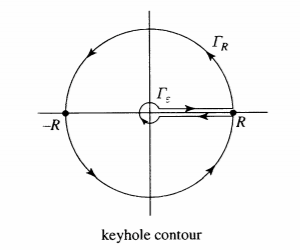
\includegraphics[width = 5.5cm]{Keyhole.PNG}
    \label{fig:key}
\end{wrapfigure}

For $\varepsilon > 0$ small and $R > 0$ large, we consider the keyhole domain $D$ consisting of $z$ in the slit plane $\C\backslash[0,\infty)$ satisfying $\varepsilon < |z| < R$. The function $f(z)$ has one pole in $D$, a double pole at $z = -1$. Using our residue rules we hav \begin{equation*}
    Res[z^a/(1+z)^2,-1] = \lim\limits_{z\rightarrow -1}a\frac{z^a}{z} = -ae^{\pi ia}
\end{equation*}
The residue theorem yields \begin{equation*}
    \int_{\partial D}f(z)dz = -2\pi iae^{\pi ia}
\end{equation*}
The integral around $\partial D$ breaks into the sum of four integrals, from $\varepsilon$ to $R$ along the top edge of the slit, around $\Gamma_R$, from $R$ back to $\varepsilon$ along the bottom edge of the slit, and around $\Gamma_{\varepsilon}$: \begin{equation*}
    \int_{\varepsilon}^R\frac{x^a}{(1+x)^2}dx + \int_{\Gamma_R}f(z)dz+\int_R^{\varepsilon}\frac{e^{2\pi ia}x^a}{(1+x)^2}dx+\int_{\Gamma_{\varepsilon}}f(z)dz
\end{equation*}
For the integrals over $\Gamma_R$ and $\Gamma_{\varepsilon}$, the ML-estimate gives \begin{align*}
    \left|\int_{\Gamma_R}\frac{z^a}{(1+z)^2}dz\right| &\leq \frac{R^a}{(R-1)^2}2\pi R\sim R^{a-1} \\
    \left|\int_{\Gamma_{\varepsilon}}\frac{z^a}{(1+z)^2}dz\right| &\leq \frac{\varepsilon^a}{(1-\varepsilon)^2}2\pi \varepsilon\sim \varepsilon^{a+1} \\
\end{align*}
Since $-1 < a < 1$, both these integrals tend to $0$ as $R\rightarrow \infty$ and $\varepsilon \rightarrow 0$. If we reverse the direction of the integral from $R$ to $\varepsilon$ and use our previous result we have \begin{equation*}
    -2\pi iae^{\pi ia} = (1-e^{2\pi ia})\int_{0}^{\infty}\frac{x^a}{(1+x)^2}dx
\end{equation*}
This yields the identity \begin{equation*}
    \int_0^{\infty}\frac{x^a}{(1+x)^2}dx = \frac{-2\pi iae^{\pi ia}}{1-e^{2\pi ia}} = \frac{2\pi ia}{e^{\pi ia}-e^{-\pi ia}} = \frac{\pi a}{\sin(\pi a)}
\end{equation*}


\begin{example}
    We wish to show that $$\int_0^{\infty}\frac{dx}{\sqrt{x}(x^2+1)} = \frac{\pi}{\sqrt{2}}$$
    Let $f(z) = \frac{z^{-1/2}}{z^2+1}$ where the root function is taken with the branch cut $[0,\infty)$. We use the keyhole contour depicted in the previous derivation. Notice $z = \pm i$ are the simple poles of $f(z)$ on the keyhole. We consider $z^{-1/2} = |z|^{-1/2}e^{-i\theta/2}$, where $\theta = \text{Arg}(z)$, so $0 < \theta < 2\pi$. Then $z^{-1/2} = \frac{1}{\sqrt{|z|}e^{i\theta/2}}$. Then, for the path along $\varepsilon$ to $R$ on the upper line $z^{-1/2} = 1/\sqrt{x}$, while on the lower line $z^{-1/2} = e^{2\pi i(-1/2)}/\sqrt{x} = -1/\sqrt{x}$. Next, we note that \begin{align*}
        \left|\int_{\Gamma_R}\frac{z^{-1/2}}{(1+z^2)}dz\right| &\leq \frac{\sqrt{R}}{(R^2-1)}2\pi R\sim R^{-1/2} \\
        \left|\int_{\Gamma_{\varepsilon}}\frac{z^{-1/2}}{(1+z^2)}dz\right| &\leq \frac{\varepsilon^{-1/2}}{(1-\varepsilon^2)}2\pi \varepsilon\sim \varepsilon^{1/2} \\
    \end{align*}
    Then as $R$ goes to infinity and $\varepsilon$ goes to $0$ both terms on the right go to $0$ so the integrals go to $0$. Now, we have the residues \begin{equation*}
        Res[1/(\sqrt{z}(z^2+1)),i] = \frac{1/(\sqrt{i}(i+i))}{1} = \frac{1}{2ie^{i\pi/4}}
    \end{equation*}
    and \begin{equation*}
        Res[1/(\sqrt{z}(z^2+1)),-i] = \frac{1/(\sqrt{-i}(-i-i))}{1} = \frac{e^{-3i\pi/4}}{-2i} 
    \end{equation*}
    Then, taking the limit we have that \begin{equation*}
        \int_{0}^{\infty}\frac{1}{\sqrt{x}(x^2+1)}dx - \int_0^{\infty}\frac{-1}{\sqrt{x}(x^2+1)}dx = 2\pi i\left(\frac{1}{2ie^{i\pi/4}}+\frac{e^{-3i\pi/4}}{-2i}\right) = \pi \left(e^{-i\pi/4}+e^{i\pi/4}\right)
    \end{equation*}
    Then simplifying we have \begin{equation*}
        \int_0^{\infty}\frac{dx}{\sqrt{x}(x^2+1)} = \pi\cos(\pi/4) = \frac{\pi}{\sqrt{2}}
    \end{equation*}
\end{example}
 

%%%%%%%%%%%%%%%%%%%% Section 1.7.5
\section{Fractional Residues}

Suppose $z_0$ is an isolated singularity of $f(z)$. For $\varepsilon > 0$ small, we consider the integral \begin{equation*}
    \int_{C_{\varepsilon}}f(z)dz
\end{equation*}
where $C_{\varepsilon}$ is the arc of the circle $|z-z_0| = \varepsilon$ subtended by a sector of aperture $\alpha$. if $\alpha = 2\pi$, then $C_{\varepsilon}$ is the full circle, and the integral is equal to $2\pi iRes[f(z),z_0]$. If the singularity of $f(z)$ is a simple pole, then we can calculate the limit of the integrals as $\varepsilon \rightarrow 0$ (as the arc encloses in on the singularity)

\begin{theorem}[Fractional Residue Theorem]
    If $z_0$ is a simple pole of $f(z)$, and $C_{\varepsilon}$ is an arc of the circle $|z-z_0| = \varepsilon$ of angle $\alpha$, then \begin{equation*}
        \lim\limits_{\varepsilon 0}\int_{C_{\varepsilon}}f(z)dz = \alpha iRes[f(z),z_0]
    \end{equation*}
\end{theorem}
\begin{proof}
    Since $f$ has a simple pole we have \begin{equation*}
        f(z) = \frac{A}{z-z_0}+g(z)
    \end{equation*}
    where $A = Res[f(z),z_0]$ and $g(z)$ is analytic at $z_0$. Then the arc $|z-z_0| = \varepsilon$ of angle $\alpha$ is parametrized by $z = z_0+\varepsilon e^{i\theta}$, $\theta_0\leq \theta\leq \theta_0+\alpha$. As the arc is a bounded subset and $g$ is analytic on the arc, it follows there exists $M > 0$ such that $|g(z)| < M$ for $|z-z_0| < \varepsilon$. Furthermore, the integral of the singular part is calculated \begin{equation*}
        \int_{C_{\varepsilon}}\frac{Adz}{z-z_0} = \int_{\theta_0}^{\theta_0+\alpha}\frac{Ai\varepsilon e^{i\theta}}{\varepsilon e^{i\theta}}d\theta = Ai\alpha
    \end{equation*}
    Note that \begin{equation*}
        \left|\int_{C_{\varepsilon}}g(z)dz\right| \leq M2\pi\varepsilon\rightarrow 0
    \end{equation*}
    by the ML-theorem, so the result follows.
\end{proof}


\begin{example}
    Let $\gamma = C_R\cup[-R,-1-\varepsilon]\cup C_{\varepsilon}\cup[-1+\varepsilon,R]$. This is a half-circular path with an idnentation around $z_0 = -1$. Here we assume $C_{\varepsilon}$ is a half-circle of radius $\varepsilon$ above the real axis. The aperature is $\pi$ (but clockwise), hence the fractional residue theorem yields \begin{equation*}
        \lim\limits_{\varepsilon\rightarrow 0}\int_{C_{\varepsilon}}\frac{dz}{(z+1)(z-i)} = -\pi iRes(1/[(z+1)(z-i)],-1) = -\pi i\frac{1}{-1-i} = \frac{\pi (i+1)}{2}
    \end{equation*}
    Now, observe that for $|z| = R > 1$, $$\left|\frac{1}{(z+1)(z-i)}\right| \leq \left|\frac{1}{||z|-|1||\cdot||z|-|i||}\right| = \frac{1}{(R-1)^2}$$
    Thus, by the ML-theorem \begin{equation*}
        \left|\int_{C_R}\frac{1}{(z+1)(z-i)}dz\right| \leq \frac{1}{(R-1)^2}\pi R \sim R^{-1}
    \end{equation*}
    which goes to $0$ as $R\rightarrow \infty$. Next, by Cauchy's Residue Theorem we have \begin{equation*}
        \int_{\gamma}\frac{1}{(z+1)(z-i)}dz = 2\pi iRes[1/[(z+1)(z-i)],i] = 2\pi i\frac{1}{i+1} = \pi(1+i)
    \end{equation*}
    Hence, as the limit $R\rightarrow \infty$ and $\varepsilon \rightarrow 0$, we find \begin{equation*}
        P.V.\int_{-\infty}^{\infty}\frac{dx}{(x+1)(x-i)} + \frac{\pi (i+1)}{2} = \pi(1+i)
    \end{equation*}
    so \begin{equation*}
        P.V.\int_{-\infty}^{\infty}\frac{dx}{(x+1)(x-i)} = \frac{\pi(i+1)}{2}
    \end{equation*}
\end{example}



%%%%%%%%%%%%%%%%%%%% Section 1.7.6
\section{Principal Values}

\begin{definition}
    An integral $\int_a^bf(x)dx$ is \Emph{absolutely convergent} if the (proper or improper) integral $\int_a^b|f(x)|dx$ is finite. The integral is \Emph{absolutely divergent} if $\int_a^b|f(x)|dx = \infty$.
\end{definition}

If an integral is absolutely divergent, there may not be an obvious way to assign a value to it (think of the relationship between absolutely and conditionally convergent series)

\begin{definition}
    Suppose $f(x)$ is continuous for $a \leq x < x_0$ and for $x_0 < x\leq b$. We define the \Emph{principal value} of the integral $\int_a^bf(x)dx$ to be \begin{equation*}
        PV\int_a^bf(x)dx = \lim\limits_{\varepsilon\rightarrow 0}\left(\int_a^{x_0-\varepsilon}+\int_{x_0+\varepsilon}^b\right)f(x)dx
    \end{equation*}
    provided that the limit exists.
\end{definition}
The principal value of the integral coincides with the usual value of the integral if $f(x)$ is absolutely integrable.



%%%%%%%%%%%%%%%%%%%% Section 1.7.7
\section{Jordan's Lemma}

\begin{lemma}[Jordan's Lemma]
    If $C_R$ is the semi-circular contour $z(\theta) = Re^{i\theta}$ for $0 \leq \theta \leq \pi$, in the upper half-plane, then \begin{equation*}
        \int_{C_R}|e^{iz}||dz| < \pi
    \end{equation*}
\end{lemma}
\begin{proof}
    Note $|e^{iz}| = e^{R\sin\theta}$ and $|dz| = Rd\theta$, so now we wish to show \begin{equation*}
        \int_{C_R}e^{R\sin\theta}d\theta < \frac{\pi}{R}
    \end{equation*}
    First, note that $\sin\theta$ is concave down on $0\leq \theta\leq \pi/2$, so the graph of $\sin\theta$ lies above the straight line connecting its endpoints, $\sin\theta >2\theta/\pi$, $0\leq\theta\leq \pi/2$. Thus \begin{align*}
        \int_0^{\pi}e^{-R\sin\theta}d\theta &= 2\int_0^{\pi/2}e^{-R\sin\theta}d\theta \leq 2 \int_0^{\pi/2}e^{-2R\theta/\pi}d\theta \\
        &= \frac{\pi}{R}\int_0^{1/R}e^{-t}dt < \frac{\pi}{R}\int_0^{\infty}e^{-t}dt = \frac{\pi}{R}
    \end{align*}
\end{proof}


\begin{example}
    Consider $\int_0^{\infty}\frac{\sin x}{x}dx$, and we calculate it using $f(z) = \frac{e^{iz}}{z}$ along an indented semi-circular path centered at $z = 0$ in the upper half plane. Notice for $|z| = R$, we have \begin{equation*}
        \left|\int_{C_R}\frac{e^{iz}}{z}dz\right| \leq \int_{C_R}\left|\frac{e^{iz}}{z}\right||dz| = \frac{1}{R}\int_{C_R}\left|e^{iz}\right||dz| < \frac{\pi}{R}
    \end{equation*}
    by Jordan's Lemma. Then as $R$ goes to $\infty$ this integral goes to $0$. Suppose $R$ goes to $\infty$ and $\varepsilon \rightarrow 0$, then Cauchy's residue and fractional residue then combine to yield \begin{equation*}
        \lim\limits_{\varepsilon\rightarrow 0}\int_{-R}^R\frac{e^{ix}}{x}dx - \pi iRes[e^{ix}/x, 0] + \lim\limits_{R\rightarrow \infty}\int_{C_R}\frac{e^{iz}}{z}dz = 0
    \end{equation*}
    hence, noting that the residue is $1$, we have \begin{equation*}
        \lim\limits_{R\rightarrow \infty}\left(\int_{-R}^{R}\frac{\cos x}{x}dx + i\int_{-R}^{R}\frac{\sin x}{x}dx\right) = \pi i
    \end{equation*}
    Note $\cos x/x$ is an odd function, hence the principal value of the integral vanishes. Thus, \begin{equation*}
        P.V.\int_{-\infty}^{\infty}\frac{\sin x}{x}dx = \pi\;\;\implies \int_0^{\infty}\frac{\sin x}{x}dx = \frac{\pi}{2}
    \end{equation*}
    since $\sin(x)/x$ is even.
\end{example}









%%%%%%%%%%%%%%%%%%%%%part.tex%%%%%%%%%%%%%%%%%%%%%%%%%%%%%%%%%%
% 
% sample part title
%
% Use this file as a template for your own input.
%
%%%%%%%%%%%%%%%%%%%%%%%% Springer %%%%%%%%%%%%%%%%%%%%%%%%%%

\begin{partbacktext}
\part{Preliminaries}
\end{partbacktext}
%%%%%%%%%%%%%%%%%%%%% chapter.tex %%%%%%%%%%%%%%%%%%%%%%%%%%%%%%%%%
%
% sample chapter
%
% Use this file as a template for your own input.
%
%%%%%%%%%%%%%%%%%%%%%%%% Springer-Verlag %%%%%%%%%%%%%%%%%%%%%%%%%%
%\motto{Use the template \emph{chapter.tex} to style the various elements of your chapter content.}
\chapter{Logarithmic Integral}
\label{LogInt} % Always give a unique label
% use \chaptermark{}
% to alter or adjust the chapter heading in the running head

%%%%%%%%%%%%%%%%%%%% Section 2.1.1
\section{The Argument Principle}


\begin{definition}
    Suppose $f(z)$ is analytic on a domain $D$. For a curve $\gamma$ in $D$ such that $f(z) \neq 0$ on $\gamma$, we refer to \begin{equation*}
        \frac{1}{2\pi i}\int_{\gamma}\frac{f'(z)}{f(z)}dz = \frac{1}{2\pi i}\int_{\gamma}d\log f(z)
    \end{equation*}
    as the \Emph{logarithmic integral} of $f(z)$ along $\gamma$.
\end{definition}

Consequently the logarithmic integral measures the change of $\log f9z)$ along the curve $\gamma$.

\begin{example}
    Consider $f(z) = (z-z_0)^n$ for $n \in \Z$. Consider the curve $\gamma$: $\gamma(t) = z_0+Re^{it}$ for $0 \leq t \leq 2\pi k$, for $k \in \Z$. $k$ denotes the \Emph{winding number} (the number of revolutions/times we wrap around the circle) of $\gamma$. Then we have the logarithmic integral \begin{align*}
        \frac{1}{2\pi i}\int_{\gamma}\frac{n(z-z_0)^{n-1}}{(z-z_0)^n}dz &= \frac{1}{2\pi i}\int_{\gamma}\frac{ndz}{z-z_0} \\
        &= \frac{1}{2\pi i}n(2\pi i k) = nk
    \end{align*}
    since we are looping around $k$ times (rather than once in Cauchy's residue theorem). Note $f(z)$ has $z=z_0$ as a zero of order $n$, so setting $k = 1$ gives the number of zeros contained in the curve.
\end{example}

\begin{theorem}
    Let $D$ be a bounded domain with piecewise smooth boundary $\partial D$, and let $f(z)$ be a meromorphic function on $D$ that extends to be analytic on $\partial D$, such that $f(z) \neq 0$ on $\partial D$. Then \begin{equation*}
        \frac{1}{2\pi i}\int_{\partial D}\frac{f'(z)}{f(z)}dz = N_0 - N_{\infty}
    \end{equation*}
    where $N_0$ is the number of zeros of $f(z)$ in $D$ and $N_{\infty}$ is the number of poles of $f(z)$ in $D$, counting multiplicities.
\end{theorem}
\begin{proof}
    Suppose $z_0$ is a zero of order $N$, so $f(z) = (z-z_0)^Nh(z)$ with $h(z_0) \neq 0$. Then $f'(z) = N(z-z_0)^{N-1}h(z)+(z-z_0)^Nh'(z)$, so \begin{equation*}
        \frac{f'(z)}{f(z)} = \frac{N}{z-z_0} + \frac{h'(z)}{h(z)}
    \end{equation*}
    so $f'(z)/f(z)$ has a simple pole at $z_0$, with residue $N$. If we sum the residues over the zeros and poles we find that the sum of the residues of $f'(z)/f(z)$ in $D$ is $N_0-N_{\infty}$, so the result follows from the residue theorem. Explicitly we have \begin{equation*}
        \frac{1}{2\pi i}\left(\underbrace{\int_{\partial D}\frac{N}{z-z_0}dz}_{simple\;pole} + \underbrace{\int_{\partial D}\frac{h'(z)}{h(z)}dz}_{analytic\implies Cauchy}\right) = \frac{1}{2\pi i}2\pi i(N+0) = N
    \end{equation*}
    Now, suppose $z_0$ is a pole of order $N$, so $f(z) = \frac{g(z)}{(z-z_0)^N}$ with $g(z_0) \neq 0$ and $g$ analytic at $z_0$. Then \begin{equation*}
        \frac{f'(z)}{f(z)} = \frac{g'(z)}{g(z)}-N\frac{1}{(z-z_0)}
    \end{equation*}
    so by Cauchy's residue theorem the integral is $-N$. The result follows by the full Cauchy residue theorem \begin{equation*}
        \frac{1}{2\pi i}\int_{\partial D}\frac{f'(z)}{f(z)}dz = \frac{1}{2\pi i}2\pi i\sum_{j=1}^kRes[f'(z)/f(z),z_k] = N_0 - N_{\infty}
    \end{equation*}
\end{proof}

\begin{remark}[Intuation for Argument Principle]
    Recall that the logarithm (as a general multivalued function) is \begin{equation*}
        \log(f(z)) = \ln|f(z)| + i\arg(f(z))
    \end{equation*}
    Then we have that \begin{equation*}
        d\log(f(z)) = d\ln|f(z)| + id\arg(f(z))
    \end{equation*}
    If $f(z) \neq 0$ on the domain, $\ln|f(z)|$ is defined and in particular $d\ln|f(z)|$ is an exact differential (and hence is trivial around curves). Thus, the logarithmic integral is really calculating $id\arg(f(z))$ around closed loops. In particular, we have \begin{equation*}
        \frac{1}{2\pi i}\int_{\gamma}d\log(f(z)) = \frac{1}{2\pi i}\int_{\gamma}d\ln|f(z)| + \frac{1}{2\pi}\int_{\gamma}d\arg(f(z))
    \end{equation*}
    If we parametrize the curve $\gamma$ by $\gamma(t) = x(t)+iy(t)$, $a \leq t \leq b$, then \begin{equation*}
        \int_{\gamma}d\ln|f(z)| = \ln|f(\gamma(b))| - \ln|f(\gamma(a))|
    \end{equation*}
    The differential $d\arg(f(z))$ is closed, but not exact. Its integral is computed by choosing a continuous single-valued determination of $\arg f(\gamma(t))$ for $a \leq t \leq b$. Then from this determination \begin{equation*}
        \int_{\gamma}d\arg(f(z)) = \arg(f(\gamma(b))) - \arg(f(\gamma(a)))
    \end{equation*}
    This is referred to as the \Emph{increase in the argument of $f(z)$ along $\gamma$}. Since any two continuous determinations of $\arg f(\gamma(t))$ differ by a constant, the increase in the argument given by the integral is independent of the continuous determination.
\end{remark}

For a bounded domain $D$ whose boundary $\partial D$ consists of a finite number of piecewise smooth closed curves with the usual orientation, we define the \Emph{increase in the argument of $f(z)$ around the boundary of $D$} to be the sum of its increases around the closed curves in $\partial D$.

\begin{theorem}
    Let $D$ be a bounded domain with piecewise smooth boundary $\partial D$, and let $f(z)$ be a meromorphic function on $D$ that extends to be analytic on $\partial D$, such that $f(z) \neq 0$ on $\partial D$. Then the increase in the argument of $f9z)$ around the boundary of $D$ is $2\pi$ times the number of zeros minus the number of poles of $f(z)$ in $D$,\begin{equation*}
        \int_{\partial D}d\arg(f(z)) = 2\pi(N_0-N_{\infty})
    \end{equation*}
\end{theorem}

\begin{example}
    Consider $f(z) = z^4 + 1$, and study $\gamma:$ $\gamma(t) = 2e^{it}$, $0 \leq t \leq 2\pi$. We want to calculate the number of zeros of the function in a circle of radius $2$ (as it has no singularities). Observe $f(\gamma(t)) = 16e^{4it}+1$, so $f(\gamma(t)) = (16\cos(4t)+1)+i\sin(4t)$. Let $x = 16\cos(4t)+1$ and $y = 16\sin(4t)$, a circle of radius $16$, centered at $1+0i$. Then the argument traverses a difference $8\pi$ on $\gamma$, so the number of roots is $4$ (as expected).
\end{example}





%%%%%%%%%%%%%%%%%%%% Section 2.1.2
\section{Rouch\'{e}'s Theorem}

There is a general principle to the effect that the number of zeros of an analytic function on a domain does not change if we make a small change in the function. 

\begin{theorem}[Rouch\'{e}'s Theorem]
    Let $D$ be a bounded domain with piecewise smooth boundary $\partial D$. Let $f(z)$ and $h(z)$ be analytic on $D\cup \partial D$. If $|h(z)| < |f(z)|$ for $z \in \partial D$, then $f(z)$ and $f(z)+h(z)$ ahve the sume number of zeros in $D$, counting multiplicities.
\end{theorem}
\begin{proof}
    By assumption $|h(z)| < |f(z)|$ we have that $f(z) \neq 0$ on $\partial D$, and that $f(z)+h(z) \neq 0$ on $\partial D$. From $f(z)+h(z) = f(z)[1+h(z)/f(z)]$, we obtain \begin{equation*}
        \arg(f(z)+h(z)) = \arg(f(z))+\arg\left(1+\frac{h(z)}{f(z)}\right)
    \end{equation*}
    Since $|h(z)/f(z)| < 1$, the values of $1+h(z)/f(z)$ lie in the right half-plane, and the increase of $\arg(1+h(z)/f(z))$ around a closed boundary curve is $0$, since we can restrict to a single-valued branch of the argument function. From the above expression we see that $\arg(f(z)+h(z))$ and $\arg f(z)$ have the same increase around $\partial D$. By the argument principle, the functions have the same number of zeros in $D$.
\end{proof}

We can think of $h(z)$ as small perturbations to the image of the curve under $f(z)$, so that the image curve will never reach the origin. That is to say, the image curve is a path or string away from the origin, and $h(z)$ are perturbations or waves in the string which are smaller in magnitude than the strings closest distance to the origin, and hence never reach the origin.


\begin{example}
    Find the number of zeros for $p(z) = z^{11}+12z^7-3z^2+z+2$ within the unit circle. Let $f(z) = 12z^7$ and $h(z) = z^{11}-3z^2+z+2$ observe for $|z| = 1$ we have $|h(z)| \leq 1+3+1+2 = 7$ and $|f(z)| = 12$. Hence, $|h(z)| < |f(z)|$, for all $z$ with $|z| = 1$. Observe that $f(z) = 12z^7$ has a zero $z = 0$ of multiplicity $7$ in the unit circle, so by Rouch\'{e}'s Theorem $p(z) = f(z)+h(z)$ has $7$ roots within the unit circle.
\end{example}

\begin{example}
    Prove that the equation $z+3+2e^z = 0$ has precisely one solution in the left-half plane. The idea here is to view $f(z) = z+3$ as being perturbed by $h(z) = 2e^z$. Clearly $f(-3) = 0$ is the only zero, and we can find a curve $\gamma$ which bounds $\mathscr{R}e(z) < 0$ and for which $|h(\gamma(t))| \leq |f(\gamma(t))|$ for all $t$ in the domain of $\gamma$, then by Rouch\'{e}'s Theorem we obtain our desired conclusion. Therefore, consider $\gamma = C_R\cup [-iR,iR]$ where $C_R$ has $z = Re^{it}$ for $\pi/2 \leq t \leq 3\pi/2$. Consider $z \in [-iR,iR]$, so $z = iy$ for $-R \leq y \leq R$ observe \begin{equation*}
        |f(z)| = |iy+3| = \sqrt{9+y^2}\;\;\&\;\;|h(z)| = |2e^{iy}| = 2
    \end{equation*}
    so $|h(z)| < |f(z)|$ for all $z \in [-iR,iR]$. Next suppose $z =x+iy \in C_R$, so $-R\leq x \leq 0$ and $-R\leq y \leq R$, with $|z| = R$. In particular, assuming $R > 5$, $R-3\leq |f(z)| = |z+3| \leq \sqrt{9+R^2}$, and $$|h(z)| = |2e^xe^{iy}| = 2e^x < 2 < R-3 < |f(z)|$$ since $-R \leq x \leq 0$. Consequently $|h(z)| < |f(z)|$ on $\gamma$ for $R > 5$, so by Rouch\'{e}'s Theorem $f(z)+h(z) = z+3+2e^z$ has only one zero in $\gamma$ for $R > 5$. Taking $R\rightarrow \infty$, the equation $z+3+2e^z$ has just one solution in the left-half plane.
\end{example}

\begin{example}[Proof of FTA]
    Consider $p(z) = a_nz^n+...+a_1z+a_0$, where $a_n \neq 0$. Let $f(z) = a_nz^n$ and hence $h(z) = a_{n-1}z^{n-1}+...+a_1z+a_0$, then $p(z) = f(z)+h(z)$. Moreover, if we choose $R > 0$ sufficiently large then $|h(z)| \leq |a_{n-1}|R^{n-1} + ... + |a_1|R+|a_0| < |a_n|R^n = |f(z)|$ for $|z| = R$ hence by Rouch\'{e}'s Theorem there are $n$-zeros of $p(z)$ in the circle of radius $R$ as $z = 0$ is a zero of multiplicity $n$ for $f(z) = a_nz^n$. Thus, every $p(z) \in \C[z]$ has $n$ zeros, counting multiplicity, on the complex plane.
\end{example}



%%%%%%%%%%%%%%%%%%%%% chapter.tex %%%%%%%%%%%%%%%%%%%%%%%%%%%%%%%%%
%
% sample chapter
%
% Use this file as a template for your own input.
%
%%%%%%%%%%%%%%%%%%%%%%%% Springer-Verlag %%%%%%%%%%%%%%%%%%%%%%%%%%
%\motto{Use the template \emph{chapter.tex} to style the various elements of your chapter content.}
\chapter{Chapter Heading}
\label{intro} % Always give a unique label
% use \chaptermark{}
% to alter or adjust the chapter heading in the running head



%%%%%%%%%%%%%%%%%%%%%part.tex%%%%%%%%%%%%%%%%%%%%%%%%%%%%%%%%%%
% 
% sample part title
%
% Use this file as a template for your own input.
%
%%%%%%%%%%%%%%%%%%%%%%%% Springer %%%%%%%%%%%%%%%%%%%%%%%%%%

\begin{partbacktext}
\part{Preliminaries}
\end{partbacktext}
%%%%%%%%%%%%%%%%%%%%% chapter.tex %%%%%%%%%%%%%%%%%%%%%%%%%%%%%%%%%
%
% sample chapter
%
% Use this file as a template for your own input.
%
%%%%%%%%%%%%%%%%%%%%%%%% Springer-Verlag %%%%%%%%%%%%%%%%%%%%%%%%%%
%\motto{Use the template \emph{chapter.tex} to style the various elements of your chapter content.}
\chapter{Approximation Theorems}
\label{Approx} % Always give a unique label
% use \chaptermark{}
% to alter or adjust the chapter heading in the running head

%%%%%%%%%%%%%%%%%%%% Section 3.1.2
\section{The Mittag-Leffler Theorem}

Recall that if $f(z)$ is a meromorphic function with pole at $z_0$, and the Laurent expansion of $f(z)$ at $z_0$ is given by $\sum_{k=-m}^{\infty}a_k(z-z_0)^k$, then the principal part $P(z)$ of $f(z)$ at $z_0$ is the sum of the terms with negative powers, $P(z) = \sum_{k=-m}^{k=-1}a_k(z-z_0)^k$. Thus $P(z)$ is a polynomial in $1/(z-z_0)$, and $f(z)-P(z)$ is analytic at $z_0$. The Mittag-Leffler theorem asserts that we can prescribe the poles and principal parts of a meromorphic function.

\begin{theorem}[Mittag-Leffler Theorem]
    Let $D$ be a domain in the complex plane. Let $\{z_k\}$ be a sequence of distinct points in $D$ with no accumulation point in $D$, and let $P_k(z)$ be a polynomial in $1/(z-z_k)$. Then there is a meromorphic function $f(z)$ on $D$ whose poles are the points $z_k$, and such that $f(z) - P_k(z)$ is analytic at $z_k$.
\end{theorem}


\begin{example}
    Consider $P_k(z) = \frac{1}{z-k}$ for $k \in \N$. Then suppose we take \begin{equation*}
        f_{naive}(z) = \sum_{k=1}^{\infty}\frac{1}{z-k}
    \end{equation*}
    and consider the domain $D = \C$. But, then $f_{naive}(0) = -\sum_{k=1}^{\infty}\frac{1}{k} = -\infty$, which is to say it is not analytic at $0$. Instead, let's take \begin{equation*}
        f(z) = \sum_{k=1}^{\infty}\left(\frac{1}{z-k}+\frac{1}{k}\right)
    \end{equation*}
    and then $f(0) = 0$, and we have analyticity on bounded sets. In particular, it converges uniformly on bounded sets by comparison the series $\sum 1/k^2$. Indeed, if $|z| \leq R$ and $k > 2R$, then $|z-k| > k/2$, so the $k$th summand is bounded by $2/k^2$.
\end{example}

Let $w_1$ and $w_2$ be two complex numbers that do not lie on the same line through the origin. Then we can construct the \Emph{Weierstrass P-Function $\mathcal{P}(z)$} associated with $w_1$ and $w_2$. This is a doubly periodic meromorphic function on the complex plane.


\begin{example}
    We wish to show the following partial fractions decomposition identity \begin{equation*}
        \frac{\pi^2}{\sin^2(\pi z)} = \sum_{k=-\infty}^{\infty}\frac{1}{(z-k)^2}
    \end{equation*}
    (note this is meromorphic on $\C$, but not on $\C^*$ since it has an essential singularity at $\infty$). Observe $\pi^2\int\csc^2(\pi z)dz = -\pi\cot(\pi z)+C$, so \begin{equation*}
        \pi\cot(\pi z) = \frac{1}{z}+2\pi\sum_{k=1}^{\infty}\frac{1}{z^2-k^2}
    \end{equation*}
\end{example}



%%%%%%%%%%%%%%%%%%%% Section 3.1.3
\section{Infinite Products}

\begin{definition}
    An \Emph{infinite product} is an expression of the form $\prod_{j=1}^{\infty}p_j$, where the $p_j$'s are complex numbers. We say that the infinite product \Emph{converges} if $p_j\rightarrow 1$ and $\sum\text{Log}p_j$ converges, where we sum only over terms for which $p_j\neq 0$. If the infinite product converges, we define its value to be $0$ if one of the $p_j$'s is $0$; otherwise, we define it to be \begin{equation*}
        \prod_{j=1}^{\infty}p_j = \exp\left(\sum_{j=1}^{\infty}\text{Log}p_j\right)
    \end{equation*}
\end{definition}

If $\prod p_j$ converges, then at most finitely many of the $p_j$'s can be $0$. This is because $p_j\rightarrow 1$. Second, if $\prod p_j$ converges, then \begin{equation*}
    \prod_{j=1}^{\infty}p_j = \lim\limits_{m\rightarrow \infty}\prod_{j=1}^mp_j
\end{equation*}
This is because $\exp(\text{Log}p_j) = p_j$.

\begin{example}
    If $p_{42} = 0$ and $p_j = 1$ for all $j \neq 42$, then $\prod_{j=1}^{\infty}p_j = 0$.
\end{example}


\begin{example}
    If $p_1 = 1-\frac{1}{j^2}$ for all $j \geq 2$, then you can directly calculate the partial products. By induction we can show \begin{equation*}
        \prod_{j=2}^n(1-1/j^2) = \frac{1}{2}\left(1+\frac{1}{n}\right)
    \end{equation*}
    Then it follows that $\prod_{j=2}^{\infty}\left(1-\frac{1}{j^2}\right) = \frac{1}{2}$. 
\end{example}

\begin{example}
    The product $\prod_{j=2}^{\infty}(1-1/j)$ is divergent despite the fact $1-\frac{1}{j}\rightarrow 1$, since $\sum_{j=2}^{\infty}\text{Log}(1-1/j)$ diverges to $-\infty$. Formally, the product diverges to $0$ since $\exp(-\infty) = 0$.
\end{example}

\begin{example}
    Consider the infinite product formed by $p_k = 1+\frac{(-1)^{k+1}}{k}$, $k \geq 1$, so \begin{align*}
        \prod_{j=1}^{\infty}\left(1+\frac{(-1)^{j+1}}{j}\right) &= (1+1/1)(1-1/2)(1+1/3)(1-1/4)... \\
        &= \lim\limits_{k\rightarrow \infty}\left[2\cdot \frac{1}{2}\cdot\frac{4}{3}\cdot \frac{3}{4}\cdot ...\cdot \left(1+\frac{(-1)^{k+1}}{k}\right)\right]
    \end{align*}
    Evidently the product of evenly many terms is $1$, so we see the product tends to $1$ as $k\rightarrow \infty$.
\end{example}

\begin{theorem}
    If $t_j \geq 0$, then $\prod(1+t_j)$ converges if and only if $\sum t_j$ converges.
\end{theorem}

\begin{definition}
    The infinite product $\prod(1+a_j)$ is said to \Emph{converge absolutely} if $a_j\rightarrow 0$ and $\sum\text{Log}(1+a_j)$ converges absolutely, where we sum over the terms for which $a_j \neq -1$. If $\prod(1+a_j)$ converges absolutely, then $\sum\text{Log}(1+a_j)$ converges and $\prod(1+a_j)$ converges.
\end{definition}

\begin{theorem}
    The infinite product $\prod(1+a_j)$ converges absolutely if and only if $\sum a_j$ converges absolutely. This occurs if and only if $\prod(1+|a_j|)$ converges.
\end{theorem}


\begin{theorem}
    Suppose that $g_k(x) = 1+h_k(x)$, $k \geq 1$, are functions on a set $E$. Suppose that there are constants $M_k > 0$ such that $\sum M_k < \infty$, and $|h_k(x)| \leq M_k$ for $x \in E$. Then $\prod_{k=1}^mg_k(x)$ converges to $\prod_k^{\infty}g_k(x)$ uniformly on $E$ as $m\rightarrow \infty$.
\end{theorem}
\begin{proof}
    (to be completed)
\end{proof}

If $G(z) = g_1(z)...g_m(z)$ is a finite product of analytic functions, then by taking logarithms and differentiating we obtain\begin{equation*}
    \frac{G'(z)}{G(z)} = \frac{g_1'(z)}{g_1(z)} + ... + \frac{g'_m(z)}{g_m(z)}
\end{equation*}
This procedure is called \Emph{logarithmic differentiation}.

\begin{theorem}
    Let $g_k(z), k \geq 1$, be analytic functions on a domain $D$ such that $\prod_{k=1}^mg_k(z)$ converges normally on $D$ to $G(z) = \prod_{k=1}^{\infty}g_k(z)$. Then \begin{equation*}
        \frac{G'(z)}{G(z)} = \sum_{k=1}^{\infty}\frac{g_k'(z)}{g_k(z)},\;\;\;\;z \in D
    \end{equation*}
    where the sum converges normally on $D$.
\end{theorem}
\begin{proof}
    (To be completed)
\end{proof}



%%%%%%%%%%%%%%%%%%%% Section 3.1.4
\section{The Weierstrass Product Theorem}

This is a companion to the Mittag-Leffler theorem, which asserts that we can prescribe the poles and principal parts of a meromorphic function, while the Weierstrass product theorem asserts that we can prescribe the zeros and poles of a meromorphic function together with their orders.

\begin{theorem}[Weierstrass Product Theorem]
    Let $D$ be a domain in the complex plane. Let $\{z_k\}$ be a sequence of distinct points of $D$ with no accumulation point in $D$, and let $\{n_k\}$ be a sequence of integers (positive or negative). Then there is a meromorphic function $f(z)$ on $D$ whose only zeros and poles are at the points $z_k$ such that the order of $f(z)$ at $z_k$ is $n_k$.
\end{theorem}
\begin{proof}
    (To be completed)
\end{proof}

\begin{example}
    Consider $\prod_{k=1}^{\infty}\left(1-\frac{z^2}{k^2}\right)$. Write $g_k(z) = 1-\frac{z^2}{k^2}$ and $h_k(z) = \frac{-z^2}{k^2}$. Suppose $|z| \leq R$ then $\left|\frac{z^2}{k^2}\right| \leq \frac{R^2}{k^2}$. Observe $\sum_{k=1}^{\infty}\frac{R^2}{k^2} = \frac{\pi R^2}{6}$ hence we find the product is uniformly convergent for $|z| < R$. But as $R$ is arbitrary we find the product $\prod_{k=1}^{m}\left(1-\frac{z^2}{k^2}\right)$ converges uniformly to $\prod_{k=1}^{\infty}\left(1-\frac{z^2}{k^2}\right)$ on $\C$.
\end{example}






%%%%%%%%%%%%%%%%%%%%% chapter.tex %%%%%%%%%%%%%%%%%%%%%%%%%%%%%%%%%
%
% sample chapter
%
% Use this file as a template for your own input.
%
%%%%%%%%%%%%%%%%%%%%%%%% Springer-Verlag %%%%%%%%%%%%%%%%%%%%%%%%%%
%\motto{Use the template \emph{chapter.tex} to style the various elements of your chapter content.}
\chapter{Special Functions}
\label{SpecFuncs} % Always give a unique label
% use \chaptermark{}
% to alter or adjust the chapter heading in the running head

%%%%%%%%%%%%%%%%%%%% Section 3.2.1
\section{The Gamma Function}

\begin{definition}
    The gamma function $\Gamma(z)$ is a meromorphic function defined on the right half-plane by \begin{equation*}
        \Gamma(z) = \int_0^{\infty}t^{z-1}e^{-t}dt,\;\;\;\;\mathscr{R}e(z) > 0
    \end{equation*}
    The integral defining $\Gamma(z)$ is absolutely convergent, and \begin{equation*}
        |\Gamma(x+iy)| \leq \Gamma(x) = \int_0^{\infty}t^{x-1}e^{-t}dt,\;\;\;\;x>0
    \end{equation*}
\end{definition}

Integrating by parts we observe that \begin{align*}
    \Gamma(z+1) &= \int_0^{\infty}e^{-t}t^zdt = -\int_0^{\infty}t^2d(e^{-t}) = -[t^2e^{-t}]_0^{\infty} + z\int_0^{\infty}e^{-t}t^{z-1}dt \\
    &= 0 + z\Gamma(z)  = z\Gamma(z),\;\;\;\;\mathscr{R}e(z) > 0
\end{align*}
Thus, we have \begin{equation*}
    \boxed{\Gamma(z+1) = z\Gamma(z),\;\;\;\;\mathscr{R}e(z) > 0}
\end{equation*}
Noting that $\Gamma(1) = 1$, and with the equation $\Gamma(2) = 1$, we obtain by induction \begin{equation*}
    \boxed{\Gamma(n+1) = n!,\;\;\;\;n\geq 0}
\end{equation*}
We use the functional equation above to extend $\Gamma(z)$ to the left half-plane as follows: apply the function equation $m$ times to obtain $\Gamma(z+m)=(z+m-1)...(z+1)z\Gamma(z)$, which we rewrite as \begin{equation*}
    \boxed{\Gamma(z) = \frac{\Gamma(z+m)}{(z+m-1)...(z+1)z}}
\end{equation*}
where the right hand side is defined and meromorphic for $\mathscr{R}e(z) > -m$, with simple poles $0,-1,...,-m+1$. By the uniqueness principle, the meromorphic extension is unique and it satisfies the functional equation. Passing to the limit as $m\rightarrow \infty$ we obtain:

\begin{theorem}
    The function $\Gamma(z)$ extends to be meromorphic on the entire complex plane, where it satisfies the functional equation $\Gamma(z+1)=z\Gamma(z)$. Its poles are simple poles at $z = 0,-1,-2,...$.
\end{theorem}

Now, define \begin{equation*}
    \Gamma_n(z) = \int_0^nt^{z-1}\left(1-\frac{t}{n}\right)^ndt,\;\;\;\;\mathscr{R}e(z) > 0, n\geq 1
\end{equation*}
Since $(1-t/n)^n \leq e^{-t}$ and $(1-t/n)^n \rightarrow e^{-t}$ for $t \geq 0$, we have \begin{equation*}
    \lim\limits_{m\rightarrow \infty}\Gamma_n(z) = \Gamma(z)
\end{equation*}

(To be continued)



%%%%%%%%%%%%%%%%%%%% Section 3.2.2
\section{Laplace Transforms}

\begin{definition}
    Let $h(s),s\geq0,$ be a continuous or piecewise continuous function on the positive real axis. The \Emph{Laplace transform of $h(s)$} is the function \begin{equation*}
        \mathcal{L}[h](z) = \int_0^{\infty}e^{-sz}h(s)ds
    \end{equation*}
    provided that the integral converges.
\end{definition}


\begin{proposition}
    If there are constants $B$ and $C$ such that $|h(s)| \leq Ce^{Bs}$ for $0 \leq s < \infty$, then the Laplace transform integral converges absolutely and defines an analytic function in the half plane $\mathscr{R}e(z) > B$. The estimate \begin{equation*}
        |\mathcal{L}[h](x+iy)| \leq C\int_0^{\infty}e^{-zs}e^{Bs}ds = \frac{C}{x-B},\;\;\;\; x > B
    \end{equation*}
    shows that $\mathcal{L}[h](z)$ is bounded on the half plane $\mathscr{R}e(z) > B+\varepsilon$ for any $\varepsilon > 0$, and $\mathcal{L}[h](z)\rightarrow 0$ as $\mathscr{R}e(z) \rightarrow \infty$.
\end{proposition}






\backmatter%%%%%%%%%%%%%%%%%%%%%%%%%%%%%%%%%%%%%%%%%%%%%%%%%%%%%%%
%%%%%%%%%%%%%%%%%%%%%% appendix.tex %%%%%%%%%%%%%%%%%%%%%%%%%%%%%%%%%
%
% sample appendix
%
% Use this file as a template for your own input.
%
%%%%%%%%%%%%%%%%%%%%%%%% Springer-Verlag %%%%%%%%%%%%%%%%%%%%%%%%%%

\appendix
\motto{All's well that ends well}
\chapter{Appendix A: Set Theory}
\section{Relations}
    
    \begin{definition}[Relation]
        A \Emph{relation} on a set $A$ is a subset $C$ of the cartesian product $A \times A$. If $C$ is a relation on $A$ we write $xCy$ to denote $(x,y) \in C$.
    \end{definition}
    

    \begin{definition}[Equivalence Relation]
        An \Emph{equivalence relation} on a set $A$ is a relation $C$ on $A$ having the following three properties: \begin{enumerate}
            \item (\Emph{Reflexivity}) $xCx$ for all $x \in A$
            \item (\Emph{Symmetry}) For $x,y \in A$, if $xCy$, then $yCx$
            \item (\Emph{Transitivity}) For $x,y,z \in A$, if $xCy$ and $yCz$, then $xCz$
        \end{enumerate}
    \end{definition}


    \begin{definition}[Equivalence Class]
        Given an equivalence relation $\sim$ on a set $A$ and an element $x$ of $A$, we define the \Emph{equivalence class} determined by $x$ to be \begin{equation}
            [x]_{\sim} := \{y \in A\vert y\sim x\}
        \end{equation}
    \end{definition}


    \begin{definition}[Partition]
        A \Emph{partition} of a set $A$ is a collection of disjoint nonempty subsets of $A$ whose union is all of $A$.
    \end{definition}



    \begin{proposition}
        Given an equivalence relation $\sim$ on a set $A$, the distinct equivalence classes of $\sim$ form a partition of $A$.
    \end{proposition}
    \begin{proof}
        (Left to the reader)
    \end{proof}

    \subsection{Order Relations}

    \begin{definition}{Order Relation}
        A relation $C$ on a set $A$ is called an \Emph{order relation} (or \Emph{simple order}, or a \Emph{linear order}) if it has the following properties: \begin{enumerate}
            \item (\Emph{Comparability}) For every $x,y \in A$ for which $x \neq y$, either $xCy$ or $yCx$
            \item (\Emph{Nonreflexivity}) For no $x \in A$ does the relation $xCx$ hold
            \item (\Emph{Transitivity}) If $xCy$ and $yCz$, then $xCz$
        \end{enumerate}
    \end{definition}

    \begin{definition}[Strict Partial Order]
        A relation $C$ on a set $A$ is called a \Emph{strict partial order relation} if it satisfies properties $2.$ and $3.$ of an order relation.
    \end{definition}

    
    \begin{definition}[Open Interval]
        If $X$ is a set and $<$ is an order relation on $X$, and if $a < b$, we use the notation $(a,b)$ to denoted the set \begin{equation*}
            \{x \in X\vert a < x < b\}
        \end{equation*}
        it is called an \Emph{open interval} in $X$. If this set is empty, we call $a$ the \Emph{immediate predecessor} of $b$ and we call $b$ the \Emph{immediate successor} of $a$.
    \end{definition}

    \begin{definition}[Order Isomorphism]
        Suppose that $A$ and $B$ are two sets with order relations $<_A$ and $<_B$ respectively. We say that $A$ and $B$ have the same \Emph{order type} if there is a bijective correspondence between them that preserves order; that is, if there exists a bijective function $f:A\rightarrow B$ such that \begin{equation*}
            a_1 <_A a_2 \implies f(a_1) <_B f(a_2)
        \end{equation*}
    \end{definition}

    \begin{definition}
        Suppose that $A$ and $B$ are two sets with order relations $<_A$ and $<_B$ respectively. Define an order relation $<$ on $A \times B$ by defining \begin{equation*}
            a_1\times b_1 < a_2\times b_2
        \end{equation*}
        if $a_1 <_A a_2$, or if $a_1 = a_2$ and $b_1 <_B b_2$. It is called the \Emph{dictionary order relation} on $A\times B$.
    \end{definition}

    
    For the next definitions, suppose that $A$ is a set ordered by the relation $<$. Let $A_0$ be a subset of $A$.


    \begin{definition}[Minima and Maxima]
        We say that the element $b \in A_0$ is the \Emph{maximum or largest element} of $A_0$ if for all $x \in A_0$, $x \leq b$. Similarly, we say that $a \in A_0$ is the \Emph{minimum or smallest element} of $A_0$ if for all $x \in A_0$, $a \leq x$. We use $\leq$ to denote $<$ or $=$.
    \end{definition}


    \begin{definition}[Supremum and Upper Bounds]
        We say that the subset $A_0$ of $A$ is \Emph{bounded above} if there is an element $b$ of $A$ such that $x \leq b$ for every $x \in A_0$; the element $b$ is called an \Emph{upper bound} for $A_0$. If the set of all upper bounds for $A_0$ has a smallest element, that element is called the \Emph{least upper bound}, or \Emph{supremum}, of $A_0$, and it is denoted by $\sup A_0$. The supremum may or may not belong to $A_0$.
    \end{definition}


    \begin{definition}[Infimum and Lower Bounds]
        We say that $A_0$ is \Emph{bounded below} if there is an element $a$ of $A$ such that $a \leq x$ for all $x \in A_0$; the element $a$ is called a \Emph{lower bound} for $A_0$. If the set of all lower bounds for $A_0$ has a largest element, that element is called the \Emph{greatest lower bound}, or \Emph{infimum}, of $A_0$, and it is denoted by $\inf A_0$. Again, the infimum may or may not belong to $A_0$.
    \end{definition}


    \begin{definition}[Least Upper Bound and Greatest Lower Bound Properties]
        An ordered set $A$ is said to have the \Emph{least upper bound property} if every nonempty subset $A_0$ of $A$ that is bounded above has a least upper bound. Analogously, the set $A$ is said to have the \Emph{greatest lower bound property} if every nonempty subset $A_0$ of $A$ that is bounded below has a greatest lower bound. 

        These two properties are in fact equivalent.
    \end{definition}


    \section{Properties of the Integers and Reals}


    \begin{definition}[Binary Operation]
        A \Emph{binary operation} on a set $A$ is a function $f:A\times A\rightarrow A$.
    \end{definition}


    \begin{construction}[The Reals]
        We assume there exists a set $\R$, called the set of \Emph{real numbers}, two binary operations $+$ and $\cdot$ on $\R$, called addition and multiplication operations, respectively, and an order relation $<$ on $\R$, such that the following properties hold: \begin{enumerate}
            \item (Associativity) For all $x,y,z \in \R$:\begin{align}
                    (x+y)+z &= x+(y+z) \\
                    (x\cdot y)\cdot z &= x\cdot (y\cdot z) 
                \end{align}
            \item (Commutivity) For all $x,y \in \R$:\begin{align}
                x+y &= y+x \\
                x\cdot y &= y \cdot x
                \end{align}
            \item (Additive Identity) There exists a unique element of $\R$ called \Emph{zero}, denoted by $0$, such that $x+0 = x$ for all $x \in \R$.
            \item (Multiplicative Identity) There exists a unique element of $\R$ called \Emph{one}, different from $0$ and denoted by $1$, such that $x\cdot 1 = x$ for all $x \in \R$.
            \item (Additive Inverses) For each $x \in\R$, $\exists y \in \R$ such that $x+y = 0$
            \item (Multiplicative Inverses) For each $x \in \R$, with $x \neq 0$, $\exists y \in \R$ such that $x\cdot y = 1$.
            \item (Distributivity) For all $x,y,z \in \R$, \begin{equation}
                    x\cdot (y+z) = (x\cdot y) + (x\cdot z)
                \end{equation}
            \item (Order Closure) If $x > y$, then $x+z > y+z$
            \item If $x > y$ and $z > 0$, then $x\cdot z > y\cdot z$
            \item (Least Upper Bound Property) The order relation $<$ has the least upper bound property.
            \item If $x < y$, there exists an element $z$ such that $x < z$ and $z < y$.
        \end{enumerate}
        Under axioms 1-6 $\R$ is known as a \Emph{field}. With the addition of axioms 7 and 8, $\R$ becomes an \Emph{ordered field}. Moreover, any set with an order relation satisfying 9 and 10 is called a \Emph{linear continuum}.
    \end{construction}

    \begin{definition}
        A subset $A$ of the real numbers is said to be \Emph{inductive} if it contains the number $1$, and if for every $x \in A$, the number $x+1$ is also in $A$. Let $\mathscr{A}$ be the collection of all inductive subsets of $\R$. Then the set $\Z_{+}$ of \Emph{positive integers} is defined by the equation \begin{equation}
            \Z_+ := \bigcap\limits_{A\in\mathscr{A}}A
        \end{equation}
        Then, $\Z_+$ is inductive, and if $A$ is an inudctive set of positive integers, then $A = \Z_+$.
    \end{definition}

    \begin{definition}[Integers]
        We define the set $\Z$ of \Emph{integers} to be the set consisting of the positive integers $\Z_+$, the number $0$, and the negatives of the elements of $\Z_+$. The set $\Q$ of quotients of integers is called the set of \Emph{rational numbers}.
    \end{definition}

    \begin{theorem}[Well-ordering Property]
        Every nonempty subset of $\Z_+$ has a smallest element.
    \end{theorem}
    \begin{proof}
        We first prove that for each $n \in \Z_+$, the following statement holds: Every nonempty subset of $\{1,...,n\}$ has a smallest element.

        Let $A$ be the set of all positive integers $n$ for which this statement holds. Then $A$ contains $1$, since if $n = 1$, the only nonempty subset of $\{1,..,n\}$ is the set $\{1\}$ itself. Then, supposing $A$ contains some $n \geq 1$, we show that it contains $n+1$. So let $C$ be a nonempty subset of $\{1,...,n+1\}$. If consists of the single element $n+1$, then that element is the smallest element of $C$. Otherwise, consider the set $C\cap\{1,...,n\}$, which is nonempty. Because $n \in A$, this set has a smallest element, which will automatically be the smallest element of $C$ also. Thus $A$ is inductive, so we conclude that $A = \Z_+$; hence the statement is true for all $n \in \Z_+$.

        To prove the theorem suppsoe $D$ is a nonempty subset of $\Z_+$. Choose an element $n$ of $D$. Then the set $A = D\cap\{1,...,n\}$ is nonempty, so that $A$ has a smallest element $k$. The element $k$ is automatically the smallest element of $D$ as well.
    \end{proof}

    \begin{theorem}[Strong Induction Principle]
        Let $A$ be a set of positive integers. Suppose that for each positive integer $n$, the statement $S_n \subseteq A$ implies the statement $n \in A$, where $S_n = \{1,...,n-1\}$. Then $A = \Z_+$.
    \end{theorem}
    \begin{proof}
        If $A$ does not equal all of $\Z_+$, let $n$ be the smallest positive integer that is not in $A$. Then every positive integer less than $n$ is in $A$ so that $S_n \subseteq A$. Our hypothesis implies that $n \in A$, contrary to assumption, so we must have that $A = \Z_+$.
    \end{proof}


    \section{Cartesian Products}

    \begin{definition}
        Let $\mathscr{A}$ be a nonempty collection of sets. An \Emph{indexing function} for $\mathscr{A}$ is a surjective function $f$ from some set $J$, called the \Emph{index set}, to $\mathscr{A}$. The collection $\mathscr{A}$, together with the indexing function $f$, is called an \Emph{indexed family of sets}. Given $\alpha \in J$, we shall denote the set $f(\alpha)$ by the symbol $A_{\alpha}$. And, we shall denote the indexed family itself by the symbol \begin{equation*}
            \{A_{\alpha}\}_{\alpha \in J}
        \end{equation*}
        which is read ``the family of all $A_{\alpha}$, as $\alpha$ ranges over $J$."
    \end{definition}

    \begin{definition}
        Suppose $f:J\rightarrow \mathscr{A}$ is an indexing function for $\mathscr{A}$, and let $f(\alpha) = A_{\alpha}$. Then we define \begin{equation*}
            \bigcup\limits_{\alpha \in J}A_{\alpha}:=\{x\;\vert\;\text{for at least one $\alpha \in J, x \in A_{\alpha}$}\} = \bigcup\limits_{A\in \mathscr{A}}A,
        \end{equation*}
        and \begin{equation*}
            \bigcap\limits_{\alpha \in J}A_{\alpha} :=\{x\;\vert\;\text{for every $\alpha \in J, x \in A_{\alpha}$}\} = \bigcap\limits_{A\in\mathscr{A}}A
        \end{equation*}
    \end{definition}


    \begin{definition}
        Let $m$ be a positive integer. Given a set $X$, we define an \Emph{$m$-tuple} of elements of $X$ to be a function \begin{equation*}
            \mathbb{x}:\{1,...,m\}\rightarrow X
        \end{equation*}
        If $\mathbb{x}$ is an $m$-tuple, we often denote the value of $\mathbb{x}$ at $i$ by the symbol $x_i$, and call it the \Emph{$i$th coordinate of $\mathbb{x}$}.

        Now, let $\{A_1,...,A_m\}$ be a family of sets indexed with the set $\{1,...,m\}$. Let $X = A_1\cup ... \cup A_m$. We define the \Emph{cartesian product} of this indexed family, denoted by \begin{equation*}
            \prod\limits_{i=1}^mA_i = A_1\times ... \times A_m
        \end{equation*}
        to be the set of all $m$-tuples, $(x_1,...,x_m)$, of elements of $X$ such that $x_i \in A_i$ for each $i$.
    \end{definition}

    \begin{definition}
        Given a set $X$, we define an \Emph{$\omega$-tuple} of elements of $X$ to be a function \begin{equation*}
            \mathbb{x}:\Z_+\rightarrow X;
        \end{equation*}
        we also call such a function a \Emph{sequence}, or an \Emph{infinite sequence}, of elements of $X$. If $\mathbb{x}$ is an $\omega$-tuple, we often denote the value of $\mathbb{x}$ at $I$ by $x_i$, and call it the $i$th coordinate of $\mathbb{x}$, as before. We denote $\mathbb{x}$ itself by $(x_1,x_2,...)$ or $(x_n)_{n\in\Z_+}$. Let $\{A_1,A_2,...\}$ be a family of sets indexed by $\Z_+$; let $X$ be the union of the sets in this family. The \Emph{cartesian product} of this indexed family of sets, denoted by \begin{equation*}
            \prod\limits_{i\in\Z_+}A_i = A_1\times A_2 \times ...
        \end{equation*}
        is defined to be the set of all $\omega$-tuples of elements of $X$ such that $x_i \in A_i$ for each $i$.
    \end{definition}

    \section{Finite Sets}

    \begin{definition}
        A set $A$ is said to be \Emph{finite} if there is a bijective correspondence of $A$ with some section of the positive integers. That is, $A$ is finite if it is empty or if there is a bijection $f:A\rightarrow \{1,...,n\}$ for some $n \in \Z_+$. In the former case we say that $A$ has \Emph{cardinality $0$}, and in the latter case we say that $A$ has \Emph{cardinality $n$}.
    \end{definition}

    \begin{lemma}
        Let $n$ be a positive integer. Let $A$ be a set; let $a_0 \in A$. Then there exists a bijective correspondence $f$ of the set $A$ with the set $\{1,...,n+1\}$ if and only if there exists a bijective correspondence $g$ of the set $A-\{a_0\}$ with the set $\{1,...,n\}$.
    \end{lemma}
    \begin{proof}
        First, suppose there is a bijection correspondence $g:A-\{a_0\}\rightarrow \{1,...,n\}$. We then define $f:A\rightarrow \{1,...,n+1\}$ by setting $f(x) = g(x)$ for $x \in A-\{a_0\}$, and $f(a_0) = n+1$. Then, $f$ is surjective for every $m \in \{1,...,n+1\}$, if $m = n+1$ then $f(a_0) = m$, while if $m \neq n+1$, $m \in \{1,...,n\}$ so there exists $x \in A-\{a_0\}$ such that $f(x) = g(x) = m$ since $g$ is a bijection. Moreover, if $f(a_1) = f(a_2)$ for $a_1,a_2 \in A$, if one of $a_1$ or $a_2$ is $a_0$, then the other must also be $a_0$ since for all $x \in A-\{a_0\}$, $f(x) \in \{1,...,n\}$. Additionally, if both $a_1 \neq a_0 \neq a_2$, then $a_1,a_2 \in A-\{a_0\}$, so $g(a_1) = f(a_1) = f(a_2) = g(a_2)$, so $a_1 = a_2$ as $g$ is injective. Thus $f$ is bijective. 

        Conversely, assume there is a bijective correspondence $f:A\rightarrow \{1,...,n+1\}$. If $f$ maps $a_0$ to the number $n+1$, we can simply take the restriction $f\rvert_{A-\{a_0\}}$. Otherwise, let $f(a_0) = m$, and let $a_1$ be a point of $A$ such that $f(a_1) = n+1$. Then $a_1 \neq a_0$. Define a new function $h:A\rightarrow \{1,...,n+1\}$ by setting $h(a_0) = n+1$, $h(a_1) = m$, and $h(x) = f(x)$ for $x \in A-\{a_0,a_1\}$. It follows that $h$ is bijective, and from the previous case, the restriction $h\rvert_{A-\{a_0\}}$ is the desired bijection.
    \end{proof}


    \begin{theorem}
        Let $A$ be a set; suppose that there exists a bijection $f:A\rightarrow \{1,...,n\}$ for some $n \in \Z_+$. Let $B$ be a proper subset of $A$. Then there exists no bijection $g:B\rightarrow \{1,...,n\}$; but (provided $B\neq \emptyset$) there does exist a bijection $h:B\rightarrow \{1,...,m\}$ for some $m < n$.
    \end{theorem}
    \begin{proof}
        The case in which $B = \emptyset$ is immediate, for there cannot exist a bijection of the empty set $B$ with the nonempty set $\{1,...,n\}$.


        We shall proceed by induction. Let $C$ be the subset of $\Z_+$ consisting of those integers $n$ for which the theorem holds. We shall show that $C$ is inductive. From this we conclude that $C = \Z_+$, so the theorem is true for all positive integers $n$.

        First we show the theorem is true for $n = 1$. In this case $A$ consists of a single element $\{a\}$, and its only proper subset $B$ is the empty set.

        Now assume that the theorem is true for $n$; we prove it true for $n+1$. Suppose that $f:A\rightarrow \{1,...,n+1\}$ is a bijection, and $B$ is a nonempty proper subset of $A$. Choose an element $a_0 \in B$ and an element $a_1 \in A-B$. We apply the preceding lemma to conclude there is a bijection \begin{equation*}
            g:A-\{a_0\}\rightarrow \{1,...,n\}
        \end{equation*}
        Now $B - \{a_0\}$ is a proper subset of $A - \{a_0\}$, for $a_1$ belongs to $A-\{a_0\}$ and not to $B-\{a_0\}$. Because we have assumed the theorem holds for the integer $n$, we conclude there exists no bijection $h:B-\{a_0\}\rightarrow \{1,...,n\}$, and either $B-\{a_0\} = \emptyset$ or there exists a bijection \begin{equation*}
            k:B-\{a_0\}\rightarrow \{1,...,p\}
        \end{equation*}
        for some $p<n$. The preceding lemma combined with the lack of a bijection $H$ implies that there is no bijection of $B$ with $\{1,...,n+1\}$. This is the first half of what we wanted to prove. To prove the second half note that if $B - \{a_0\} = \emptyset$, there is a bijection of $B$ with the set $\{1\}$; while if $B-\{a_0\} \neq \emptyset$, we can apply the preceding lemma, along with the induction hypothesis to conclude that there is a bijection of $B$ with $\{1,...,p+1\}$. In either case, there is a bijection of $B$ with $\{1,...,m\}$ for some $m < n+1$, as desired. The induction principle now shows that the theorem is true for all $n \in \Z_+$.
    \end{proof}

    \begin{corollary}
        If $A$ is finite, there is no bijection of $A$ with a proper subset of itself.
    \end{corollary}
    \begin{proof}
        Assume that $B$ is a proper subset of $A$ and that $f:A\rightarrow B$ is a bijection. By assumption there is a bijection $g:A\rightarrow \{1,...,n\}$ for some $m$. The composite $g \circ f^{-1}$ is then a bijection of $B$ with $\{1,...,n\}$. This contradicts the preceding theorem.
    \end{proof}


    \begin{corollary}
        $\Z_+$ is not finite.
    \end{corollary}
    \begin{proof}
        The function $f:\Z_+\rightarrow \Z_+ -\{1\}$ defined by $f(n) = n+1$ is a bijection of $\Z_+$ with a proper subset of itself, so it cannot be finite.
    \end{proof}


    \begin{corollary}
        The cardinality of a finite set $A$ is uniquely determined by $A$.
    \end{corollary}
    \begin{proof}
        For the sake of contradiction, let $m < n$. Suppose there are bijections $f:A\rightarrow \{1,...,n\}$ and $g:A\rightarrow \{1,...,m\}$. Then the composite $g\circ f^{-1}:\{1,...,n\}\rightarrow \{1,...,m\}$ is a bijection of the finite set with a proper subset of itself, contradiction the previous corollary.
    \end{proof}


    \begin{corollary}
        If $B$ is a subset of the finite set $A$, then $B$ is finite. If $B$ is a proper subset of $A$, then the cardinality of $B$ is less than the cardinality of $B$.
    \end{corollary}
    

    \begin{corollary}
        Let $B$ be a nonempty set. Then the following are equivalent:\begin{enumerate}
            \item $B$ is finite.
            \item There is a surjective function from a section of the positive integers into $B$.
            \item There is an injective function from $B$ into a section of the positive integers.
        \end{enumerate}
    \end{corollary}
    \begin{proof}
        ($(1)\implies (2)$) Since $B$ is nonempty, there is, for some $n$, a bijection function $f:\{1,...,n\}\rightarrow B$ by definition, which is inherently surjective.

        ($(2)\implies (3)$) If $f:\{1,...,n\}\rightarrow B$ is surjective, define $g:B\rightarrow \{1,...,n\}$ by the equation \begin{equation*}
            g(b) = \text{smallest element of } f^{-1}(\{b\})
        \end{equation*}
        Because $f$ is surjective, the set $f^{-1}(\{b\})$ is nonempty; then the well-ordering property of $\Z_+$ tells us that $g(b)$ is uniquely defined. The map $g$ is injective, for if $b \neq b'$, then the sets $f^{-1}(\{b\})$ and $f^{-1}(\{b'\})$ must be disjoint, so their smallest elements must be different.


        ($(3)\implies (1)$) If $g:B\rightarrow \{1,...,n\}$ is injective, then changing the range of $g$ gives a bijection of $B$ with a subset of $\{1,...,n\}$. It follows from the preceding corollary that $B$ is finite.
    \end{proof}


    \begin{corollary}
        Finite unions and finite cartesian products of finite sets are finite.
    \end{corollary}
    \begin{proof}
        We first show that if $A$ and $B$ are finite, so is $A\cup B$. If $A$ or $B$ is empty the result is immediate. Otherwise, there are bijections $f:\{1,...,m\}\rightarrow A$ and $g:\{1,...,n\}\rightarrow B$ for some choice of $m$ and $n$. Define a function $h:\{1,...,m+n\}\rightarrow A\cup B$ by setting $h(i) = f(i)$ for $i \in \{1,...,m\}$ and $h(i) = g(i-m)$ for $i \in \{m+1,...,m+n\}$. Evidently, for all $a \in A$ there exists $i \in \{1,...,m\}$ such that $h(i) = f(i) = a$ since $f$ is a bijection. Moreover, for all $b \in B$ there exists $i \in \{1,...,n\}$ such that $h(i+m) = g(i) = b$, since $g$ is a bijection. Hence $h$ is surjective so by the previous corollary $A\cup B$ is finite.

        Now we show by induction that finiteness of the sets $A_1,...,A_n$ implies finiteness of their union. This result is immediate for $n=1$. Assuming it true for $n-1$ we note that $A_1\cup...\cup A_n$ is the union of two finite sets $A_1\cup ... \cup A_{n-1}$ and $A_n$ by the induction hypothesis, so the result of the preceding paragraph applies.

        Now, we show that the cartesian product of two finite sets $A$ and $B$ is finite. Given $a \in A$, the set $\{a\}\times B$ is finite, being in bijective correspondence with $B$. The set $A \times B$ is the union of these sets; since there are only finitely many of them, $A\times B$ is a finite union of finite sets and thus finite.

        Now we argue by induction that the finiteness of the sets $A_1,...,A_n$ implies the finiteness of $A_1\times ...\times A_n$. For $n = 1$ this result is immediate. Assuming it true for $n-1$, consider $A_1\times ... \times A_n$. Note that this is in bijective correspondence with the set $(A_1\times ... \times A_{n-1})\times A_n$, which is the cross product of two finite sets by the induction hypothesis. Hence by the previous argument $(A_1\times ... \times A_{n-1})\times A_n$ is finite. In particular, since it is in bijective correspondence with $A_1\times ... \times A_n$, this cartesian product is also finite.
    \end{proof}



    \section{Countable and Uncountable Sets}

    
    \begin{definition}
        A set $A$ is said to be \Emph{infinite} if it is not finite. It is said to be \Emph{countably infinite} if there is a bijective correspondence \begin{equation*}
            f:A\rightarrow \Z_+
        \end{equation*}
    \end{definition}


    \begin{definition}
        A set is said to be \Emph{countable} if it is either finite or countably infinite. A set that is not countable is said to be \Emph{uncountable}.
    \end{definition}

    \begin{theorem}
        Let $B$ be a nonempty set. Then the following are equivalent:\begin{enumerate}
            \item $B$ is countable.
            \item There is a surjective function $f:\Z_+\rightarrow B$.
            \item There is an injective function $g:B\rightarrow \Z_+$.
        \end{enumerate}
    \end{theorem}
    \begin{proof}
        ($(1)\implies(2)$) Suppose that $B$ is countable. If $B$ is countably infinite there is a bijection $f:\Z_+\rightarrow B$ by definition, and we are done. If $B$ is finite, there is a bijection $h:\{1,...,n\}\rightarrow B$ for some $n \geq 1$. We can extend $h$ to a surjection $f:\Z_+\rightarrow B$ by defining \begin{equation*}
            f(i) = \left\{\begin{array}{ll} h(i) & \text{for } 1\leq i \leq n \\
            h(1) & \text{for } i > n \end{array}\right.
        \end{equation*}

        ($(2)\implies (3)$) Let $f:\Z_+\rightarrow B$ be a surjection. Define $g:B\rightarrow \Z_+$ by the equation \begin{equation*}
            g(b) = \text{smallest element of $f^{-1}(\{b\})$}
        \end{equation*}
        Because $f$ is surjective, $f^{-1}(\{b\})$ is nonempty; thus $g$ is well defined by the well-ordering of $\Z_+$. The map $g$ is injective, for if $b \neq b'$, the sets $f^{-1}(\{b\})$ and $f^{-1}(\{b'\})$ are disjoint, so their elements are different.

        ($(3)\implies (1)$) Let $g:B\rightarrow \Z_+$ be an injection; we wish to show $B$ is countable. By changing the range of $g$, we can obtain a bijection of $B$ with a subset of $\Z_+$. Thus to prove our result it suffices to show that every subset of $\Z_+$ is countable. So let $C$ be a subset of $\Z_+$.

        If $C$ is finite, it is countable by definition. For $C$ an infinite subset of $\Z_+$ we provide a proof in the lemma to follow.
    \end{proof}


    \begin{lemma}
        If $C$ is an infinite subset of $\Z_+$, then $C$ is countably infinite.
    \end{lemma}
    \begin{proof}
        We define a bijection $h:\Z_+\rightarrow C$. We proceed by induction. Define $h(1)$ to be the smallest element of $C$; it exists because every nonempty subset $C$ of $\Z_+$ has a smallest element by the well-ordering of $\Z_+$. Then assuming that $h(1),...,h(n-1)$ are defined, define \begin{equation*}
            h(n) = \text{smallest element of } [C-h(\{1,...,n-1\})].
        \end{equation*}
        The set $C-h(\{1,...,n-1\})$ is not empty; for if it were empty, then $h:\{1,...,n-1\}\rightarrow C$ would be surjective, so that $C$ would be finite. Thus $h(n)$ is well defined. By induction we have defined $h(n)$ for all $n \in \Z_+$.


        To show that $h$ is injective consider $m \neq n$. Without loss of generality take $m < n$, and note that $h(m) \in \{h(\{1,...,n-1\})$, whereas $h(n)$, by definition, is not. Hence $h(n) \neq h(m)$.

        To show that $h$ is surjective, let $c$ be any element of $C$; we show that $c$ lies in the image set of $h$. First note that $h(\Z_+)$ cannot be contained in the finite set $\{1,...,c\}$ because $h(\Z_+)$ is infinite since $h$ is injective. Therefore, there is an $n \in \Z_+$, such that $h(n) > c$. Let $m$ be the smallest element of $\Z_+$ such that $h(m) \geq c$. Then for all $i < m$, we must have that $h(i) < c$. Thus, $c$ does not belong to the set $h(\{1,...,m-1\})$. Since $h(m)$ is defined as the smallest element of the set $C-h(\{1,...,m-1\})$, we must have that $h(m) \leq c$. Putting the two inequalities together, we have $h(m) = c$, as desired.
    \end{proof}


    \begin{definition}[Principle of Recursive Definition]
        Let $A$ be a set. Given a formula theat defines $h(1)$ as a unique element of $A$, and for $i > 1$ defines $h(i)$ uniquely as an element of $A$ in terms of the values of $h$ for positive integers less than $i$, this formula deterimes a unique function $h:\Z_+\rightarrow A$.
    \end{definition}


    \begin{corollary}
        A subset of a countable set is countable.
    \end{corollary}
    \begin{proof}
        Suppose $A \subseteq B$, where $B$ is countable. There is an injection of $f$ of $B$ into $\Z_+$; the restriction of $f$ to $A$ is an injection of $A$ into $\Z_+$.
    \end{proof}


    \begin{corollary}
        The set $\Z_+\times \Z_+$ is countably infinite.
    \end{corollary}
    \begin{proof}
        It suffices to construct an injective map $f:\Z_+\times \Z_+\rightarrow \Z_+$. We define $f$ by the equation $$f(n,m) = 2^n3^m$$ It is clear that $f$ is injective. For suppose that $2^n3^m = 2^p3^q$. If $n < p$, then $3^m = 2^{p-n}3^q$, contradicting the fact that $3^m$ is odd for all $m$. Therefore, $n = p$. As a result, $3^m = 3^q$. Then if $m < q$, it follows that $1 = 3^{q-m}$, another contradiction. Hence $m = q$.
    \end{proof}


    \begin{theorem}
        A countable union of countable sets is countable.
    \end{theorem}
    \begin{proof}
        Let $\{A_n\}_{n\in J}$ be an indexed family of countable sets, where the index set $J$ is either $\{1,...,N\}$ or $\Z_+$. Assume that each set $A_n$ is nonempty, for convenience.

        Because $A_n$ is countable, we can choose, for each $n$, a surjective function $f_n:\Z_+\rightarrow A_n$. Similarly, we can choose a surjective function $g:\Z_+\rightarrow J$. Now define \begin{equation*}
            h:\Z_+\times \Z_+\rightarrow \bigcup\limits_{n\in J}A_n
        \end{equation*}
        by the equation $h(k,m) = f_{g(k)}(m)$. Then indeed $h$ is surjective. Since $\Z_+\times\Z_+$ is in bijective correspondence with $\Z_+$, the countability of the union follows.
    \end{proof}

    \begin{theorem}
        A finite product of countable sets is countable.
    \end{theorem}
    \begin{proof}
        First let us show that the product of two countable sets is $A$ and $B$ is countable. The result is trivial if $A$ or $B$ is empty. Otherwise, choose surjective functions $f:\Z_+\rightarrow A$ and $g:\Z_+\rightarrow B$. Then the function $h:\Z_+\times \Z_+\rightarrow A\times B$ defined by $h(n,m) = (f(n),g(m))$ is surjective, so that $A\times B$ is countable.


        In general, we proceed by induction. Assuming that $A_1\times ... \times A_{n-1}$ is countable if each $A_i$ is countable, we prove the same thing for the product $A_1\times ... \times A_n$. FIrst, note that there is a bijective correspondence \begin{equation*}
            g:A_1\times ... \times A_n\rightarrow (A_1\times ... \times A_{n-1})\times A_n
        \end{equation*}
        defined by the equation \begin{equation*}
            g(x_1,...,x_n) = ((x_1,...,x_{n-1}),x_n)
        \end{equation*}
        Becuase the set $A_1\times ... A_{n-1}$ is countable by the induction hypothesis and $A_n$ is countable by assumption, the product of these two sets is countable, as proved in the preceding paragraph. We conclude that $A_1\times ... \times A_n$ is countable as well.
    \end{proof}

    It is not true that the countable product of countable sets is countable. Indeed, this fails almost immediately.

    \begin{theorem}
        Let $X$ denote the two element set $\{0,1\}$. Then the set $X^{\omega}$ is uncountable.
    \end{theorem}
    \begin{proof}
        We show that given any function $$g:\Z_+\rightarrow X^{\omega}$$ $g$ is not surjective. For this, let us denote $g(n)$ by \begin{equation*}
            g(n_ = (x_{n1},x_{n2},...,x_{nm},...)
        \end{equation*}
        where each $x_{ij}$ is either $0$ or $1$. Then we define an element $\mathbf{y} = (y_1,y_2,...,y_n,...)$ of $X^{\omega}$ by \begin{equation*}
            y_n = \left\{\begin{array}{ll} 0 & \text{if } x_{nn} = 1,\\ 1 & \text{if } x_{nn} = 0\end{array}\right.
        \end{equation*}
        Now $\mathbf{y}$ is an element of $X^{\omega}$, and $\mathbf{y}$ does not lie in the image of $g$; given $n$, the point $g(n)$ and the point $\mathbf{y}$ differ in at least one coordinate, namely, the $n$th. Thus, $g$ is not surjective.
    \end{proof}


    \begin{theorem}
        Let $A$ be a set. There is no injective map $f:\mathscr{P}(A)\rightarrow A$, and there is no surjective map $g:A\rightarrow \mathscr{P}(A)$. 
    \end{theorem}
    \begin{proof}
        In general, if $B$ is a nonempty set, the existence of an injective map $f:B\rightarrow C$ implies the existence of a surjective map $g:C\rightarrow B$; one defines $g(c) = f^{-1}(\{c\})$ for each $c \in \ran(f)$, and define $g$ arbitrarily on the rest of $C$.

        Therefore, it suffices to show that given a map $g:A\rightarrow \mathscr{P}(A)$, the map $g$ is not surjective. For each $a \in A$, the image $g(a)$ of $a$ is a subset o f$A$, which may or may not contain the point $a$ itself. Let $B$ be the subset of $A$ consisting of all those points $a$ such taht $g(a)$ does not contain $a$; \begin{equation*}
            B=\{a\;\vert\;a\in A-g(a)\}
        \end{equation*}
        Now, $B$ may be empty, or it may be all of $A$, but that does not matter. We assert that $B$ is a subset of $A$ that does not lie in the image of $g$. For suppose that $B = g(a_0)$ for some $a_0 \in A$. Does $a_0$ belong to $B$ or not? By definition of $B$, \begin{equation*}
            a_0 \in B \iff a_0 \in A-g(a_0) \iff a_0 \in A-B
        \end{equation*}
        In either case, we have a contradiction.
    \end{proof}
    

    \section{Principle of Recursive Definition}

    \begin{remark}
        Given the infinite subset $C$ of $\Z_+$, let us consider the following recursion formula for a function $h:\Z_+\rightarrow C$:\begin{equation*}
            \begin{array}{cl} h(1) &= \text{ smallest element of $C$}, \\
            h(i) &= \text{ smallest element of } [C-h(\{1,...,i-1\})]\;\;\text{ for } i > 1.
            \end{array} \tag{$(\star)$}
        \end{equation*}
        We shall prove that a unqiue such function $h$ exists in steps.
    \end{remark}

    \begin{lemma}{}{recexist}
        Given $n \in \Z_+$, there exists a function \begin{equation*}
            f:\{1,...,n\}\rightarrow C
        \end{equation*}
        that satisfies $(\star)$ for all $i$ in its domain.
    \end{lemma}
    \begin{proof}
        Let $A$ be the set of all $n$ for which the lemma holds. We show that $A$ is inductive. It then follows that $A = \Z_+$.


        The lemma is true for $n=1$, since the function $f:\{1\}\rightarrow C$ defined by the equation $f(1) = $ smallest element of $C$ satsfies $(\star)$ by the well ordering of $\Z_+$.

        Suppose the lemma to be true for $n-1$, we prove it true for $N$. By hypothesis there is a function $f':\{1,...,n-1\}\rightarrow C$ satisfying $(\star)$ for all $i$ in its domain. Define $f:\{1,...,n\}\rightarrow C$ by the equations \begin{align*}
            f(i) &= f'(i)\;\;\text{ for } i\in\{1,...,n-1\} \\
            f(n) &= \text{ smallest element of } [C-f'(\{1,...,n-1\})]
        \end{align*}
        Since $C$ is infinite, $f'$ is not surjective; hence the set $C-f'(\{1,...,n-1\})$ is nonempty, and $f(n)$ is well defined. Note that this definition does not define in terms of itself but in terms of the given function $f'$, so it is acceptable. Then by construction $f$ satisfies $(\star)$ for all $i$ in its domain since $f'$ does, and for $i = n$, $f(n) = $ smallest element of $[C-f'(\{1,...,n-1\})]$ and $f'(\{1,...,n-1\}) = f(\{1,...,n-1\})$.
    \end{proof}

    \begin{lemma}{}{recunique}
        Suppose that $f:\{1,...,n\}\rightarrow C$ and $g:\{1,...,m\}\rightarrow C$ both satisfy $(\star)$ for all $i$ in their respective domains. Then $f(i) = g(i)$ for all $i$ in both domains.
    \end{lemma}
    \begin{proof}
        Suppose towards a contradiction that the conclusion does not hold. Let $I$ be the smallest integer for which $f(i) \neq g(i)$. The integer $i$ is not $1$, because \begin{equation*}
            f(1) = \text{ smallest element of $C$ } = g(1),
        \end{equation*}
        by $(\star)$. Now, for all $j < i$, we have $f(j) = g(j)$. Because $f$ and $g$ satisfy $(\star)$, \begin{align*}
            f(i) &= \text{ smallest element of } [C-f(\{1,...,i-1\})] \\
            g(i) &= \text{ smallest element of } [C-g(\{1,...,i-1\})]
        \end{align*}
        Since $f(\{1,...,i-1\}) = g(\{1,...,i-1\})$, we have $f(i) = g(i)$, contrary to the choice of $i$.
    \end{proof}


    \begin{theorem}
        There exists a unique function $h:\Z_+\rightarrow C$ satisfying $(\star)$ for all $i \in \Z_+$.
    \end{theorem}
    \begin{proof}
        By Lemma \ref{lem:recexist}, there exists for each $n$ a function that maps $\{1,...,n\}$ into $C$ and satisfies $(\star)$ for all $i$ in its domain. Given $n$, Lemma \ref{lem:recunique} shows that this function is unique. Let $f_n:\{1,...,n\}\rightarrow C$ denote this unique function.


        We define a function $h:\Z_+\rightarrow C$ by defining its rule to be the union $U$ of the rules of the functions $f_n$. The rule for $f_n$ is a subset of $\{1,...,n\}\times C$; therefore, $U$ is a subset of $\Z_+\times C$. We must show that $U$ is a rule for a function $h:\Z_+\rightarrow C$.

        The integer $i$ lies in the domain of $f_n$ if and only if $n \geq i$. Therefore, the set of elements of $U$ of which $i$ is the first coordinate is precisely the set of all pairs of the form $(i,f_n(i))$ for $n \geq i$. Now Lemma \ref{lem:recunique} says that $f_n(i) = f_m(i)$ if $n,m \geq i$. Therefore, all these elements of $U$ are equal; that is, there is only one element of $U$ that has $i$ as its first coordinate.

        To show that $h$ satisfies $(\star)$ we note that \begin{align*}
            &h(i) = f_n(i)\;\;\text{ for } i \leq n \\
            &f_n\text{ satisfies $(\star)$ for all $i$ in its domain}
        \end{align*}
        The proof of uniqueness mirrors that of Lemma \ref{lem:recunique}.
    \end{proof}

    \begin{theorem}[Principle of Recursive Definition]
        Let $A$ be a set; let $a_0$ be an element of $A$. Suppose $\rho$ is a function that assigns, to each function $f$ mapping a nonempty section of the positive integers into $A$, an element of $A$. Then there exists a unique function \begin{equation*}
            h:\Z_+\rightarrow A
        \end{equation*}
        such that \begin{equation*}
            \begin{array}{cl} h(1) &= a_0, \\
                h(i) &= \rho(h\rvert_{\{1,...,i-1\}})\;\;\text{ for } i > 1.
            \end{array} \tag{$(\star)$}
        \end{equation*}
        The formula $(\star)$ is called a \Emph{recursion formula} for $h$. 
    \end{theorem}
    \begin{proof}
        (Left to the reader)
    \end{proof}


    \section{Infinite Sets and the Axiom of Choice}


    \begin{theorem}\label{thm:infequivs}
        Let $A$ be a set. The following statements about $A$ are equivalent:\begin{enumerate}
            \item There exists an injective function $f:\Z_+\rightarrow A$
            \item There exists a bijection of $A$ with a proper subset of itself
            \item $A$ is infinite
        \end{enumerate}
    \end{theorem}
    \begin{proof}
        $1.\implies 2.$ Assume there is an injective function $f:\Z_+\rightarrow A$. Let the image set $f(\Z_+)$ be denoted by $B$; and let $f(n)$ be denoted by $a_n$. Because $f$ is injective, $a_n\neq a_m$ if $n \neq m$. Define \begin{equation*}
            g:A\rightarrow A-\{a_1\}
        \end{equation*}
        by the equations \begin{align*}
            g(a_n) = a_{n+1}\;\;\text{ for }a_n \in B, \\
            g(x) = x\;\;\text{ for } x \in A-B
        \end{align*}
        By construction $g$ is surjective, and by the injectivity of $f$, $g$ is also injective and hence a bijection.

        $2.\implies 3.$ This result is the contrapositive of a previous result on finite sets.


        $3.\implies 1.$ Assume that $A$ is infinite and construct ``by induction" an injective function $f:\Z_+\rightarrow A$. First, since the set $A$ is nonempty, we choose a point $a_1 \in A$, and define $f(1) = a_1$. Then, assuming that we have defined $f(1),...,f(n-1)$, we wish to define $f(n)$. The set $A-f(\{1,...,n-1\})$ is not empty, for if it were empty the map $f:\{1,...,n-1\}\rightarrow A$ would be a surjection and $A$ would be finite. Hence, we can choose an element of the set $A-f(\{1,...,n-1\})$ and define $f(n)$ to be this element. ``Using the induction principle," we have defined $f$ for all $n \in \Z_+$.

        It follows by construction that $f$ is injective, for if $m < n$, then $f(m) \in f(\{1,...,n-1\})$, while by definition $f(n) \notin f(\{1,...,n-1\})$. Therefore, $f(n) \neq f(m)$.
    \end{proof}

    \begin{remark}
        What we have just done is not really a proof. Indeed, on the basis of the properties of set theory we have discussed thus far, it is not possible to prove this theorem. Precisely, before we have described certain allowable methods for specifying sets:\begin{enumerate}
            \item Defining a set by listing its elements, or by taking a given set $A$ and specifying a subset $B$ of it by giving a property that the elements of $B$ are to satisfy.
            \item Taking unions or intersections of the elements of a given collection of sets, or taking the difference of two sets.
            \item Taking the set of all subsets of a given set.
            \item Taking cartesian products of sets.
        \end{enumerate}
    \end{remark}

    \begin{axiom}[Axiom of Choice]
        Given a collection $\mathscr{A}$ of disjoint nonempty sets, there exists a set $C$ consisting of exactly one element from each element of $\mathscr{A}$. That is, a set $C$ such that $C$ is contained in the union of the elements of $\mathscr{A}$, and for each $A \in \mathscr{A}$, the set $C\cap A$ is a singleton.
    \end{axiom}

    \begin{lemma}[Existence of a Choice Function]
        Given a collection $\mathscr{B}$ of nonempty sets (not necessarily disjoint), there exists a function \begin{equation}
            c:\mathscr{B}\rightarrow \bigcup\limits_{B\in\mathscr{B}}B
        \end{equation}
        such that $c(B) \in B$ for each $B \in \mathscr{B}$. The function $c$ is called a \Emph{choice function} for the collection $\mathscr{B}$.
    \end{lemma}
    \begin{proof}
        Given an element $B$ of $\mathscr{B}$, we define a set $B'$ by $B' :=\{(B,x)\vert x \in B\}$. That is, $B'$ is the collection of all ordered pairs where the first coordinate of the ordered pair is the set $B$ and the second coordinate is an element of $B$. The set $B'$ is a subset of the cartesian product \begin{equation*}
            \mathscr{B}\times \bigcup\limits_{B\in \mathscr{B}}B
        \end{equation*}
        Because $B$ contains at least one element $x$, the set $B'$ contains at least the element $(B,x)$, so it is nonempty.

        Now, we claim that if $B_1$ and $b_2$ are two different sets in $\mathscr{B}$, then the corresponding sets $B'_1$ and $B'_2$ are disjoint. Indeed, for the typical element $(B_1,x_1) \in B_1'$ and $(B_2,x_2) \in B_2'$, $(B_1,x_1) \neq (B_2,x_2)$ as $B_1 \neq B_2$. Now let us form the collection \begin{equation*}
            \mathscr{C} :=\{B'\vert B \in \mathscr{B}\};
        \end{equation*}
        it is a collection of disjoint nonempty subsets of \begin{equation*}
            \mathscr{B}\times \bigcup\limits_{B\in \mathscr{B}}B
        \end{equation*}
        By the choice axiom, there exists a set $c$ consisting of exactly one element from each element of $\mathscr{C}$. Then $c$ contains exactly one element from each set $B'$, so for each $B \in \mathscr{B}$, the set $c$ contains exactly one ordered pair $(B,x)$ whose first coordiante is $B$. Thus $c$ is indeed the rule for a function from the collection $\mathscr{B}$ to the set $\bigcup_{B\in\mathscr{B}}B$. Finally, if $(B,x) \in c$, then $x$ belongs to $B$, so tha t$c(B) \in B$, as desired.
    \end{proof}




    \begin{proof}[Proof of Theorem \ref{thm:infequivs}]
        Given the infinite set $A$, we wish to construct an injective function $f:\Z_+\rightarrow A$. Let us form the collection $\mathscr{B}$ of all nonempty subsets of $A$. The lemma just proved asserts the existence of a choice function for $\mathscr{B}$; that is, that is a function \begin{equation*}
            c:\mathscr{B}\rightarrow \bigcup\limits_{B\in\mathscr{B}}B = A
        \end{equation*}
        such that $c(B) \in B$ for each $B \in \mathscr{B}$. Let us now define a function $f:\Z_+\rightarrow A$ by the recursion formula \begin{align*}
            f(1) &= c(A) \\
            f(i) &= c(A-f(\{1,...,i-1\}))\;\;\text{ for } i >1
        \end{align*}
        Because $A$ is infinite, the set $A-f(\{1,...,i-1\})$ is nonempty; therefore, the right side of this equation is well defined. Since this formula defines $f(i)$ uniquely in terms of $f\rvert_{\{1,...,i-1\}}$, the principle of recursive definition applies. We conclude that there exists a unieq function $f:\Z_+\rightarrow A$ satisfying $(\star)$ for all $i \in \Z_+$. Injectivity of $f$ follows as before.
    \end{proof}



    \section{Well-Ordered Sets}

    
    \begin{definition}
        A set $A$ with an order relation $<$ is said to be \Emph{well-ordered} if every nonempty subset of $A$ has a smallest element.
    \end{definition}

    \begin{example}
        $\Z_+$ is the prototypical example of a well-ordered set. Moreover, $\Z_+\times \Z_+$ with the dictionary order is a well-ordered set.
    \end{example}

    \begin{remark}
        Here are two ways of constructing well-ordered sets:\begin{enumerate}
            \item If $A$ is a well-ordered set, then any subset of $A$ is well-ordered in the restricted order relation.
            \item If $A$ and $B$ are well-ordered sets, then $A\times B$ is well-ordered in the dictionary order.
        \end{enumerate}
        It follows that $\Z_+\times(\Z_+\times \Z_+)$ is well ordered, and in general for $n \in \Z_+$, $(\Z_+)^n$ is well-ordered.
    \end{remark}

    \begin{theorem}
        Every nonempty finite ordered set has the order type of a section $\{1,...,n\}$ of $\Z_+$, so it is well-ordered.
    \end{theorem}
    \begin{proof}
        First, we show that every finite ordered set $A$ has a largest element. If $A$ has one element this is trivial. Supposing it true for sets having $n-1$ elements, let $A$ have $n$ elements and let $a_0 \in A$. Then $A-\{a_0\}$ has a largest element $a_1$, and $\max(\{a_0,a_1\})$ is the largest element of $A$.


        Second, we show there is an order-preserving bijection of $A$ with $\{1,...,n\}$ for some $n$. If $A$ has one element this fact is immediate. Suppose that it is true for sets having $n-1$ elements. Let $b$ be the largest element of $A$. By hypothesis there is an order preserving bijection \begin{equation*}
            f':A-\{b\}\rightarrow \{1,...,n-1\}
        \end{equation*}
        Define an order preserving bijection $f:A\rightarrow \{1,...,n\}$ by settign $f(x) = f'(x)$ for all $x \neq b$, and $f(b) = n$.
    \end{proof}

    \begin{theorem}[Well-ordering Theorem]
        If $A$ is a set, there exists an order relation on $A$ that is a well-ordering.
    \end{theorem}


    \begin{corollary}
        There exists an uncountable well-ordered set.
    \end{corollary}


    \begin{definition}
        Let $X$ be a well-ordered set. Given $\alpha \in X$, let $S_{\alpha}$ denote the set \begin{equation*}
            S_{\alpha} := \{x \in X\vert x < \alpha\}
        \end{equation*}
        It is called the \Emph{section} of $X$ by $\alpha$.
    \end{definition}


    \begin{lemma}
        There exists a well-ordered set $A$ having a largest element $\Omega$, such that the section $S_{\Omega}$ of $A$ by $\Omega$ is uncountable, but every other section of $A$ is countable.
    \end{lemma}
    \begin{proof}
        Let $B$ be an uncountable well-ordered set. Let $C$ be the well-ordered set $\{1,2\}\times B$ in the dictionary order; then some section of $C$ is uncountable. Indeed, the section of $C$ by any element of the form $2\times b$ is uncountable. Let $\Omega$ be the smallest element of $C$ for which the section of $C$ by $\Omega$ is uncountable. Then let $A$ consist of this section along with the element $\Omega$.
    \end{proof}

    \begin{remark}
        $S_{\Omega}$ is an uncountable well-ordered set every section of which is countable. Its order type is in fact uniquely determined by this condition, and we call it a \Emph{minimal uncountable well-ordered set}. Furthermore, we denote the well-ordered set $A = S_{\Omega}\cup\{\Omega\}$ by $\overline{S}_{\Omega}$.
    \end{remark}

    \begin{theorem}
        If $A$ is a countable subset of $S_{\Omega}$, then $A$ has an upper bound in $S_{\Omega}$.
    \end{theorem}
    \begin{proof}
        Let $A$ be a countable subset of $S_{\Omega}$. For each $a \in A$, the section $S_a$ is countable. Therefore, the union $B = \bigcup_{a\in A}S_a$ is also countable. Since $S_{\Omega}$ is uncountable, the set $B$ is notall of $S_{\Omega}$; let $x$ be a point of $S_{\Omega}$ that is not in $B$. Then $x$ is an upper bound for $A$. For if $x < a$ for some $a \in A$, then $x$ belongs to $S_a$ and hence to $B$, contrary to choice.
    \end{proof}


    \section{The Maximum Principle}

    \begin{definition}
        Given a set $A$, a relation $\prec$ on $A$ is called a \Emph{strict partial order} on $A$ if it has the following two properties: \begin{enumerate}
            \item (Nonreflexivity) The relation $a \prec a$ never holds,
            \item (Transitivity) If $a \prec b$ and $b \prec c$, then $a \prec c$.
        \end{enumerate}
    \end{definition}

    \begin{theorem}[The Maximum Principle]
        Let $A$ be a set; let $\prec$ be a strict partial order on $A$. Then there exists a maximal simply ordered subset $B$ of $A$.
    \end{theorem}


    \begin{example}
        If $\mathscr{A}$ is any collection of sets, the relation $\subset$ (proper subset) is a strict partial order on $\mathscr{A}$. 
    \end{example}

    \begin{definition}
        Let $A$ be a set and let $\prec$ be a strict partial order on $A$. If $B$ is a subset of $A$, an \Emph{upper bound} of $B$ is an element $c \in A$ such that for every $b \in B$, either $b = c$ or $b \prec c$. A \Emph{maximal element} of $A$ is an element $m$ of $A$ such that for no element of $a$ of $A$ does the relation $m \prec a$ hold.
    \end{definition}

    \begin{lemma}[Zorn's Lemma]
        Let $A$ be a set that is strictly partially ordered. If every simply ordered subset of $A$ has an upper bound in $A$, then $A$ has a maximal element.
    \end{lemma}

    \begin{remark}
        A \Emph{partial order} on a set $A$ is a relation $\preceq$ such that $a \preceq b$ if either $a = b$ or $a \prec b$ where $\prec$ is a strict partial order on $A$.
    \end{remark}




%%%%%%%%%%%%%%%%%%%%%%%acronym.tex%%%%%%%%%%%%%%%%%%%%%%%%%%%%%%%%%%%%%%%%%
% sample list of acronyms
%
% Use this file as a template for your own input.
%
%%%%%%%%%%%%%%%%%%%%%%%% Springer %%%%%%%%%%%%%%%%%%%%%%%%%%

\Extrachap{Glossary}


Use the template \emph{glossary.tex} together with the Springer document class SVMono (monograph-type books) or SVMult (edited books) to style your glossary\index{glossary} in the Springer layout.


\runinhead{glossary term} Write here the description of the glossary term. Write here the description of the glossary term. Write here the description of the glossary term.

\runinhead{glossary term} Write here the description of the glossary term. Write here the description of the glossary term. Write here the description of the glossary term.

\runinhead{glossary term} Write here the description of the glossary term. Write here the description of the glossary term. Write here the description of the glossary term.

\runinhead{glossary term} Write here the description of the glossary term. Write here the description of the glossary term. Write here the description of the glossary term.

\runinhead{glossary term} Write here the description of the glossary term. Write here the description of the glossary term. Write here the description of the glossary term.
%
\Extrachap{Solutions}

\section*{Problems of Chapter~\ref{intro}}

\begin{sol}{prob1}
The solution\index{problems}\index{solutions} is revealed here.
\end{sol}


\begin{sol}{prob2}
\textbf{Problem Heading}\\
(a) The solution of first part is revealed here.\\
(b) The solution of second part is revealed here.
\end{sol}


\printindex

%%%%%%%%%%%%%%%%%%%%%%%%%%%%%%%%%%%%%%%%%%%%%%%%%%%%%%%%%%%%%%%%%%%%%%

\end{document}





